%!TEX root = ThesisEx.tex
% \resetdatestamp
\chapter{Listener-aware recommendation}\label{ch:6-listener-aware-music-recommendation}
% \section{Recommender systems}\label{section:ch5}
% \vspace{0.05cm}
\graphicspath{{./figs/ch8/}}
% Converting implicit preference to explicit 1 to 5 level liking scale
% Should I explain here how I'm using user-side features or in the  chapter of context-aware recommendation?
% More information on user profiling: EchoNest Taste profile (in alpha release) https://web.archive.org/web/20160312191903/http://developer.echonest.com/docs/v4/catalog.html
% Diversity - measures the overall diversity of a fan’s listening by mapping the overall distance across the musical styles of the listener. Mainstreamness - measures the overall familiarity of a user’s listening activity to determine preference for either mainstream or more obscure music. Freshness - measures listening habits to determine how much a user cares about new album releases vs. sticking with older music. Adventurouness - measures how open the listener is to music outside of his or her musical comfort zone.
% Also check the white paper ~\autocite{echonest13how}, and how EN is profiling ``high value'' listeners' interests such as: social causes, concerts, beer, wine, and liquor, green/eco, outdoor, fashion, sports, fitness, travel, parenting, and personal finance.
% \subsection{Recommending music according to profiles of listeners}
The modelling of users for multimedia information retrieval systems has been a research topic since the first International Symposium on Music Information Retrieval (ISMIR) in 2000. 
In that meeting, \textcite{chai00using} observed that to create modern, more efficient, and personalised music information retrieval systems, the modelling of users would be necessary because many features of multimedia content delivery are perceptual and user-dependent. 
As a result, they proposed a language capable of expressing different types of user information that also allowed the interoperability between music information retrieval systems to share these user profiles.


Sixteen years after the first ISMIR meeting, the landscape of music consumption has changed enormously and the idea of sharing user models and profiles now seems quite na\"{\i}ve.  The rise and fall of peer-to-peer networking led to the reinvention of the music industry: the paradigmatic music pro\-duct was no longer a full album in a physical format, but individual music files available in online digital music stores. 
Thanks to the miniaturisation of portable media players and also to almost ubiquitous Internet access, a change of paradigm in music consumption has happened again, and people seem to not want to pay for individual tracks. Instead, they are willing to pay for services that allow them to access, search, and discover music items---artists, albums, or tracks---within large repositories \autocite{wikstrom13music}. 

On-demand digital music streaming services are currently the fastest growing sector of the global music industry \autocite{ifpi15global} and in 2015, the digi\-tal revenues that these systems generate overtook the income from physical music goods for the first time in music industry history \autocite{ifpi16global}. 
The on-demand music streaming landscape these days seems to be a lucrative battlefield, and one on which many companies want to compete.
% For Ek, the streaming model is more like modern advertising 
% Spotify's streaming patent \autocite{ehn12peer}
However, most of the profits from the streaming model of business do not rely on the number of subscribers to these systems, providing the best experience to access music, or on finding the best next song that a listener would like to hear. 
Since the majority of the listeners' accounts in music streaming services use the ``free'' or ``freemium'' business model---advertisement-supported basic streaming services---a large share of the income of music and media streaming companies comes from targeting ads more precisely at listeners \autocite{rutter16music}.
All in all, people are no longer passive observers but direct participants in the battlefield that is the digital media and music streaming landscape.
% \todo{DB: I'm not sure what you mean here}
In fact, the traded goods in this business are individual profiles and psycographic traits (i.e, interests, lifestyle, personality, values) which are extracted from correlating their listening habits with their sociographic characteristics \autocite{prey16musica}. 
As a result, listeners are the source of information, but they also are the final target for all the commercials these companies are making money from. 


The main research question of this dissertation is about the degree of impact of using demographic, profiling, and contextual features from listeners in improving the performance of automated music recommendation systems.
However, these features may also be used to profile and model a user's traits for potentially musically-unrelated purposes, such as the aforementioned ad customisation.
Since the customised promotion of products and services is driving the music industry business, while not directly discussed, the research presented in this dissertation may have applications beyond automatic music recommendation.

In Section \ref{sec:6-listener-demographic-profiling-and-contextual-features} we will describe a set of listening behavioural features that we developed to characterise and profile listeners. We will formalise them and show how they can be used to find patterns at the country and age-group levels. In conjunction with self-declared demographic features and basic forms of listening context extracted from  aggregated listening patterns, in Section \ref{sec:6-experiment-implementation} we will evaluate if the use of these signals improve the accuracy of a recommendation model.



\section{\textit{User-centric} features}\label{sec:6-listener-demographic-profiling-and-contextual-features}
Traditional automated music recommendation systems embedded in most music streaming services still typically rely on the accuracy of statistical models learned only from the past preferences of users on music items. 
However, \textcite{lee15user, fuller16elucidating} found that  there are different types of listeners in terms of how they consume music, and so it seems reasonable to think that each type of listener needs a different type of recommendation.
Therefore, additional sources of data such as the demographic attributes of listeners, and their listening behaviour and context, may encode information about people and their listening habits and preferences that can be used to improve the performance of a music recommendation model. 




Now we will discuss the impact of using demographic and profiling characteristics---\\which in the context of this dissertation have been referred to as \emph{user-side} or \emph{user-centric} features---in improving the accuracy of a music recommendation model.
User-centric features were extracted from listeners' self-declared demographic data and a set of custom-built profiling features characterizing their music listening behaviour. 
Models based on latent factors and all combinations of user-side features were learnt by using data from the Music Listening Histories Dataset (MLHD) described in Chapter 4.
% ~\ref{ch:5-music-listening-histories-dataset}
Finally, music listening histories were aggregated into different time spans to evaluate if the accuracy of the models changed in different periods of listening. 





\subsection{Music listening behavioural features design}\label{sub:ch6-profiling-features-design}
We hypothesised that by better understanding the listening behaviour of people, we will be able to more accurately model a user's needs. Hence, the recommendation of music items can be tailored to each listener, and the prediction accuracy will likely improve. 
    
A set of five computational features tailored to characterise listening behaviours were described in \textcite{echonest13how}, and presented as part of The Echo Nest Taste Profile API project.\footnote{Deprecated after Spotify acquired The Echo Nest, but available through Internet Archive's Wayback Machine at \url{https://web.archive.org/web/20150707212616/http://developer.echonest.com/docs/v4/tasteprofile.html}} These features were developed to identify the listening characteristics that best described a listener, allowing music streaming services to recognise ``high-value'' users (i.e., the highly engaged listeners of a music service) and groups of users with similar patterns of music listening behaviour. According to The Echo Nest, the ultimate goal of these profiling features was to identify ``psychographic characteristics'' of the high-value users to monetise this group of listeners via ``targeted advertising.''
% Is not better if I don't present them for more novelty?
The set of features that The Echo Nest designed to describe listeners were \textit{adventurousness} (i.e., how open the listener is to music outside their ``musical comfort zone''), \textit{diversity} (i.e., how varied the listener’s preferred styles and genres are), \textit{freshness} (i.e., the listener's preference for new and recent artists versus older music), \textit{locality} (i.e., describes the spread, worldwide, of where the listener's preferred artists come from), and \textit{mainstreamness} (i.e, the listener's affinity for well-known artists versus obscure artists). 
Although The Echo Nest provided detailed documentation about how they calculated their custom-designed acoustic features based on the work by \textcite{jehan05creating}, they did not provide any implementation details about how they calculated their listening profile features. 
The Echo Nest's Million Song Dataset Taste Profile subset supplied listening information for a large amount of listeners, but only in the form of playcounts without any temporal information. 
Finally, The Echo Nest API\footnote{The Echo Nest API is not available any more. However, the API documentation can still be accessed at \url{https://web.archive.org/web/20160407081912/http://developer.echonest.com/docs/v4/index.html#overview}} was taken down shortly after Spotify acquired The Echo Nest, and so there is no way of correlating a song's feature values with a listener's behavioural features using their API. The obscurantism about how they calculated these listening behavioural characteristics may be an indication of the high value of this information.

In order to evaluate if music listening behavioural characteristics can be used to improve the performance of a music  recommendation model beyond plain collaborative filtering (CF), \textcite{schedl15tailoring} proposed another set of custom-designed features that attempted to describe aspects of music listening behaviours in relation to music artists.
Although the authors computed continuous values for their listening-centric user features, they grouped the listeners into categorical levels according to their feature values, perhaps losing some information in this process. Then, they compared the performance of single and combined recommendation algorithms by varying the number of recommended artists between one and 1,000.
As a result, they evaluated different recommendation approaches only in regard to the set of more popular artists with listeners grouped in fixed listening categories. 
Some of the features proposed by the authors considered only the number of playcounts, but did not consider the ranking of the music items within the overall ranking or within each listener's ranking. Therefore, biases in the distribution of items could be amplified during the feature computation.
The authors planned to integrate their listening behaviour features as user-centric features directly into recommendation algorithms based on matrix factorisation, however there are no publications with this implementation so far.

Now we will describe our efforts attempting to represent some characteristics of music listening behaviours. Attending to the conceptual design and implementation details of listening behavioural features on previous studies, we used continuous feature values to express the precise value of a certain listening behaviour characteristic in relation to a music item, and we considered the position of the music items within each listener's  ranking as well as the overall ranking . Finally, we integrated these feature values directly into a recommendation model based on matrix factorisation (see Subsection \ref{sub:matrix}) in order to predict the preference values on all available items.

We restricted ourselves to designing four novel features to describe listener behaviours: \textit{exploratoryness}, \textit{mainstreamness}, \textit{genderedness}, and \textit{fringeness}. 
Values for these features were computed for the three types of  music items in the dataset: tracks, albums, and artists. Therefore, each listener's listening was described by a vector of 12 values.
In the following sections we will describe the goals behind each of these features, give details about their implementation, visualise data patterns, and provide some analysis of the results. 

\subsubsection{Exploratoryness}\label{subsec:exploratoryness}
	To represent how much a listener explores different music instead of listening to the same music repeatedly we developed the \emph{exploratoryness} feature. 

	For each user $x$'s listening history, let 
    $L$ be the number of submitted music logs,
    $S_k$ be all submitted music items of type $k$, where $k$=\{tracks, albums, artists\},
	$s_{k,i}$ be the number of music logs for the given music item key $k$ at ranking $i$. 
    The ranking was the ordered set of music items,  from the most highly listened to the less frequently listened item. This information was computed directly from the music items frequencies within each listening history for each listener.
    We computed the exploratoryness $e_{x,k}$ for listener $x$ on a given music item of type $k$ as:
    	\vspace{1em}
		\begin{equation}
			\abovedisplayskip=2pt plus 3pt minus 9pt
			\label{eq:exploratoryness}
			e_{x,k} = 1 - \frac{1}{L}\sum_{i=1}^{S_k}{\frac{s_{k,i}}{i}}
		\end{equation}
    




Exploratoryness  returns a normalised value, with values closer to zero for  users listening to the same music item again and again, and values closer to one for users with more exploratory listening behaviour. 
% ~\citeauthor{baur12listening} found that one of the listening factors that influences music preference is what they called variety, how often songs, albums, and artists are repeated. Since their approach was based on principal component analysis, there was no mathematical formulation for this features and also there was no explanation about how they arrived to this concept.




% \begin{figure*}[t]
% % \hspace{-1.5em}
% 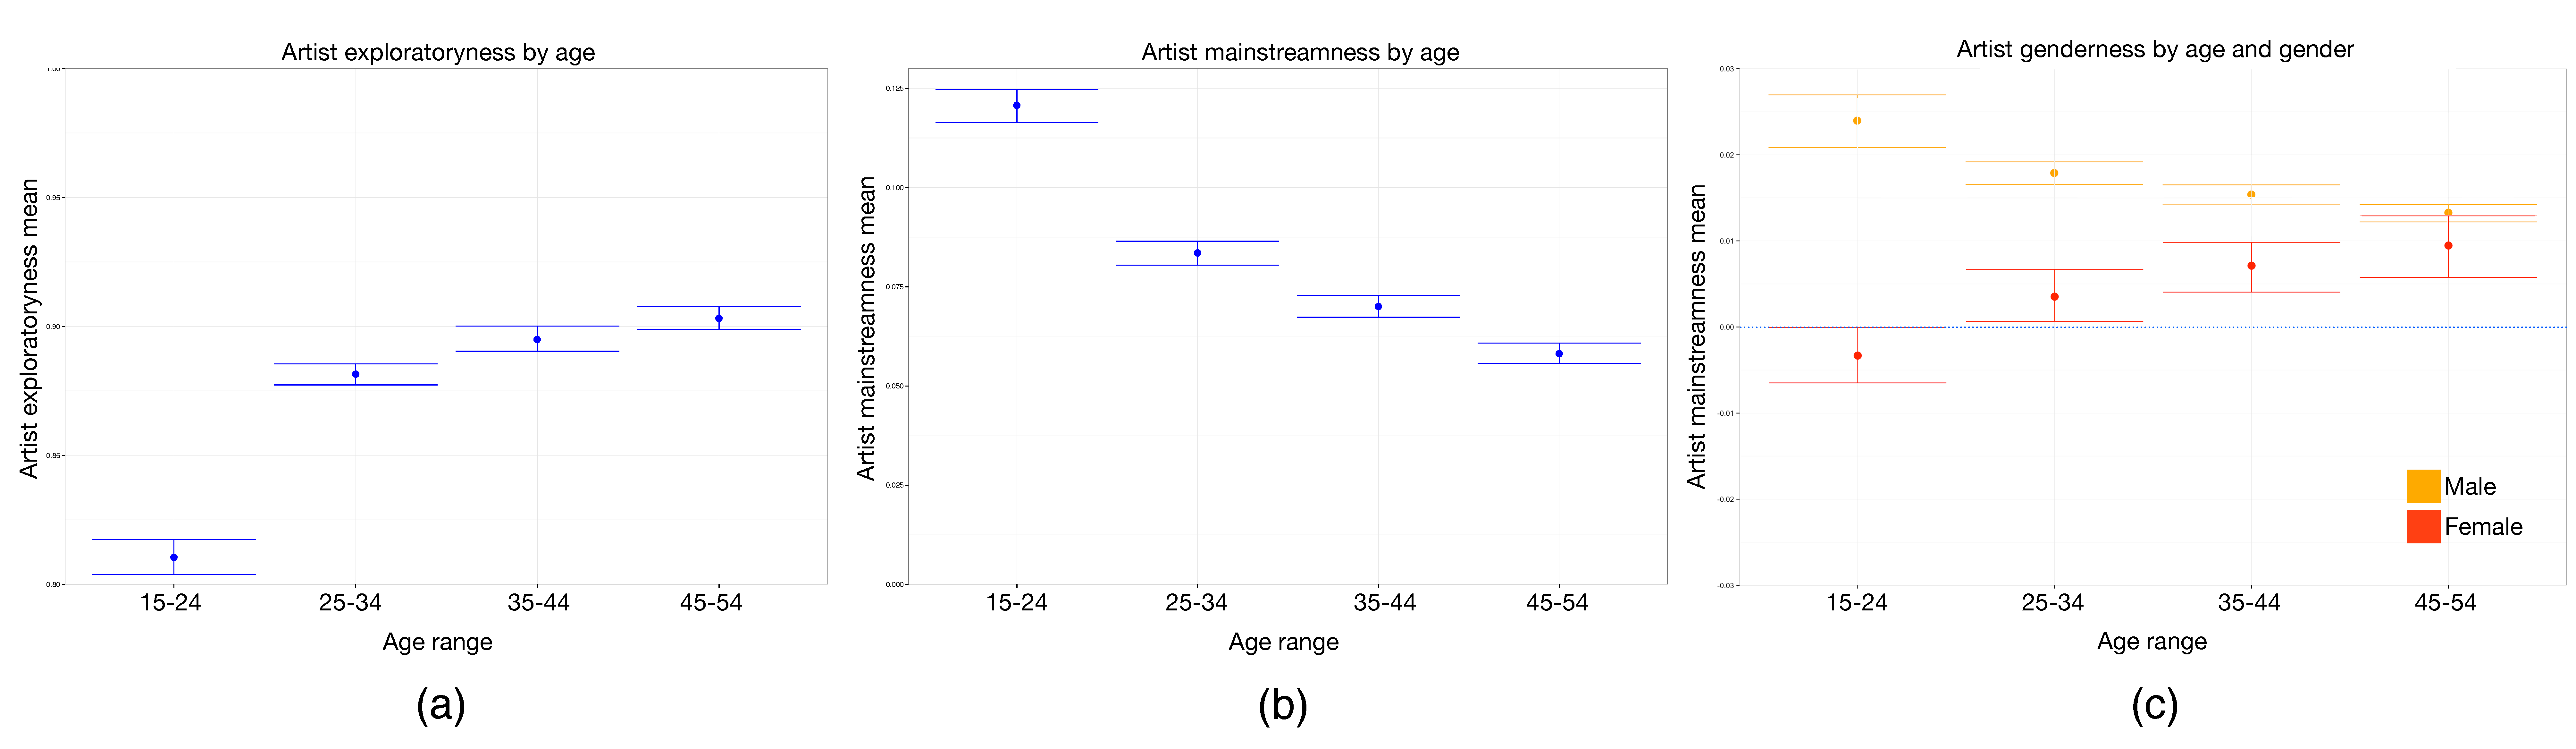
\epsfig{file=2_3_features_age_groups.pdf, width=\textwidth, keepaspectratio}
% % \caption{Feature extraction for listeners in the dataset. (a) Artist exploratoryness of listeners by age, (b) track mainstreamness of listeners by age, (c) artist genderedness of listeners by age and gender. In all cases error bars show $\pm$1 SD and 95\% ci.}
% \caption{Feature means and 95\% CI bars for a random group of listeners in our dataset. Each age group has 1000 listeners and error bars were calculated by taking 1000 populations replicated from the original sample using bootstrap. (a) Artist exploratoryness by age group of listeners, (b) artist mainstreamness by age groups of listeners, and (c) artist genderedness by age group and gender of listeners.}

% \label{fig:3_features}
% \end{figure*}	


% Fig. \ref{fig:3_features}

	% \begin{figure*}[t]
	% 	% \hspace{-1.5em}
	% 	\epsfig{file=plots/3_features.png, width=\textwidth, keepaspectratio}
	% 	\caption{Feature extraction for listeners in the dataset. (a) Artist exploratoryness of listeners by age, (b) track mainstreamness of listeners by age, (c) artist genderedness of listeners by age and gender.}
	% 	\label{fig:3_features}
	% \end{figure*}	





\subsubsection{Mainstreamness}\label{subsec:mainstreamness}
	With the goal of expressing how similar a listener's listening history is to what everyone else listened to, we developed the \emph{mainstreamness} feature. It analyses a listener's ranking of music items, and compares it with the overall ranking of artists, albums, or tracks, looking for the position of co-occurrences. %Music logs in the database without IDs are not considered.
	

	For each user $x$'s listening history, let 
	$N$ be the number of logs of the music item ranked first in the overall ranking,
    $L$ be the number of submitted music logs,
%     $S$ be all music items keys for any of the three types, 
	$S_k$ be all submitted music items of type $k$, where $k$=\{tracks, albums, artists\},
%     $s_i$ be the number of music logs of music item ranked at position $i$ , and 
	$s_{k,i}$ be the number of music logs for the given music item key $k$ at ranking $i$, and
%     $o_i$ be the number of music logs in the overall ranking of music items ranked at position $i$. 
	$o_{k,i}$ be the number of music logs in the overall ranking of music item type $k$ ranked at position $i$.
    	We defined the mainstreamness feature $m_{x,k}$ for listener $x$ on a given music item of type $k$ as:
		\begin{equation}
% 			\abovedisplayskip=2pt plus 3pt minus 9pt
			\label{eq:mainstreamness}
			m_{x,k}=\frac{1}{N L}\sum_{i=1}^{S_k}{s_{k,i}}{o_{k,i}}
		\end{equation}



Listening histories of people with a music item's ranking similar to the overall ranking receive mainstreamness values closer to one. Listeners' mainstreamness whose ranking differs more from the overall ranking receive values closer to zero.
As mainstreamness depends upon the overall ranking of music items we computed the overall ranking from all music logs in MLHD for the three music entities in the dataset. In Table \ref{table:artist_ranking} we show the first 20 artists and their total number of logs in the ranking of artists. 

\graphicspath{{./figs/ch6/}}
\begin{table}[!h]
% \vspace{1em}
\centering
\caption[20 top-ranked artists in the MLHD dataset]{20 top-ranked artists in the MLHD dataset. The ``Total logs'' column refers to the total number of logs, in millions, for the particular artist in the dataset.}\label{table:artist_ranking}
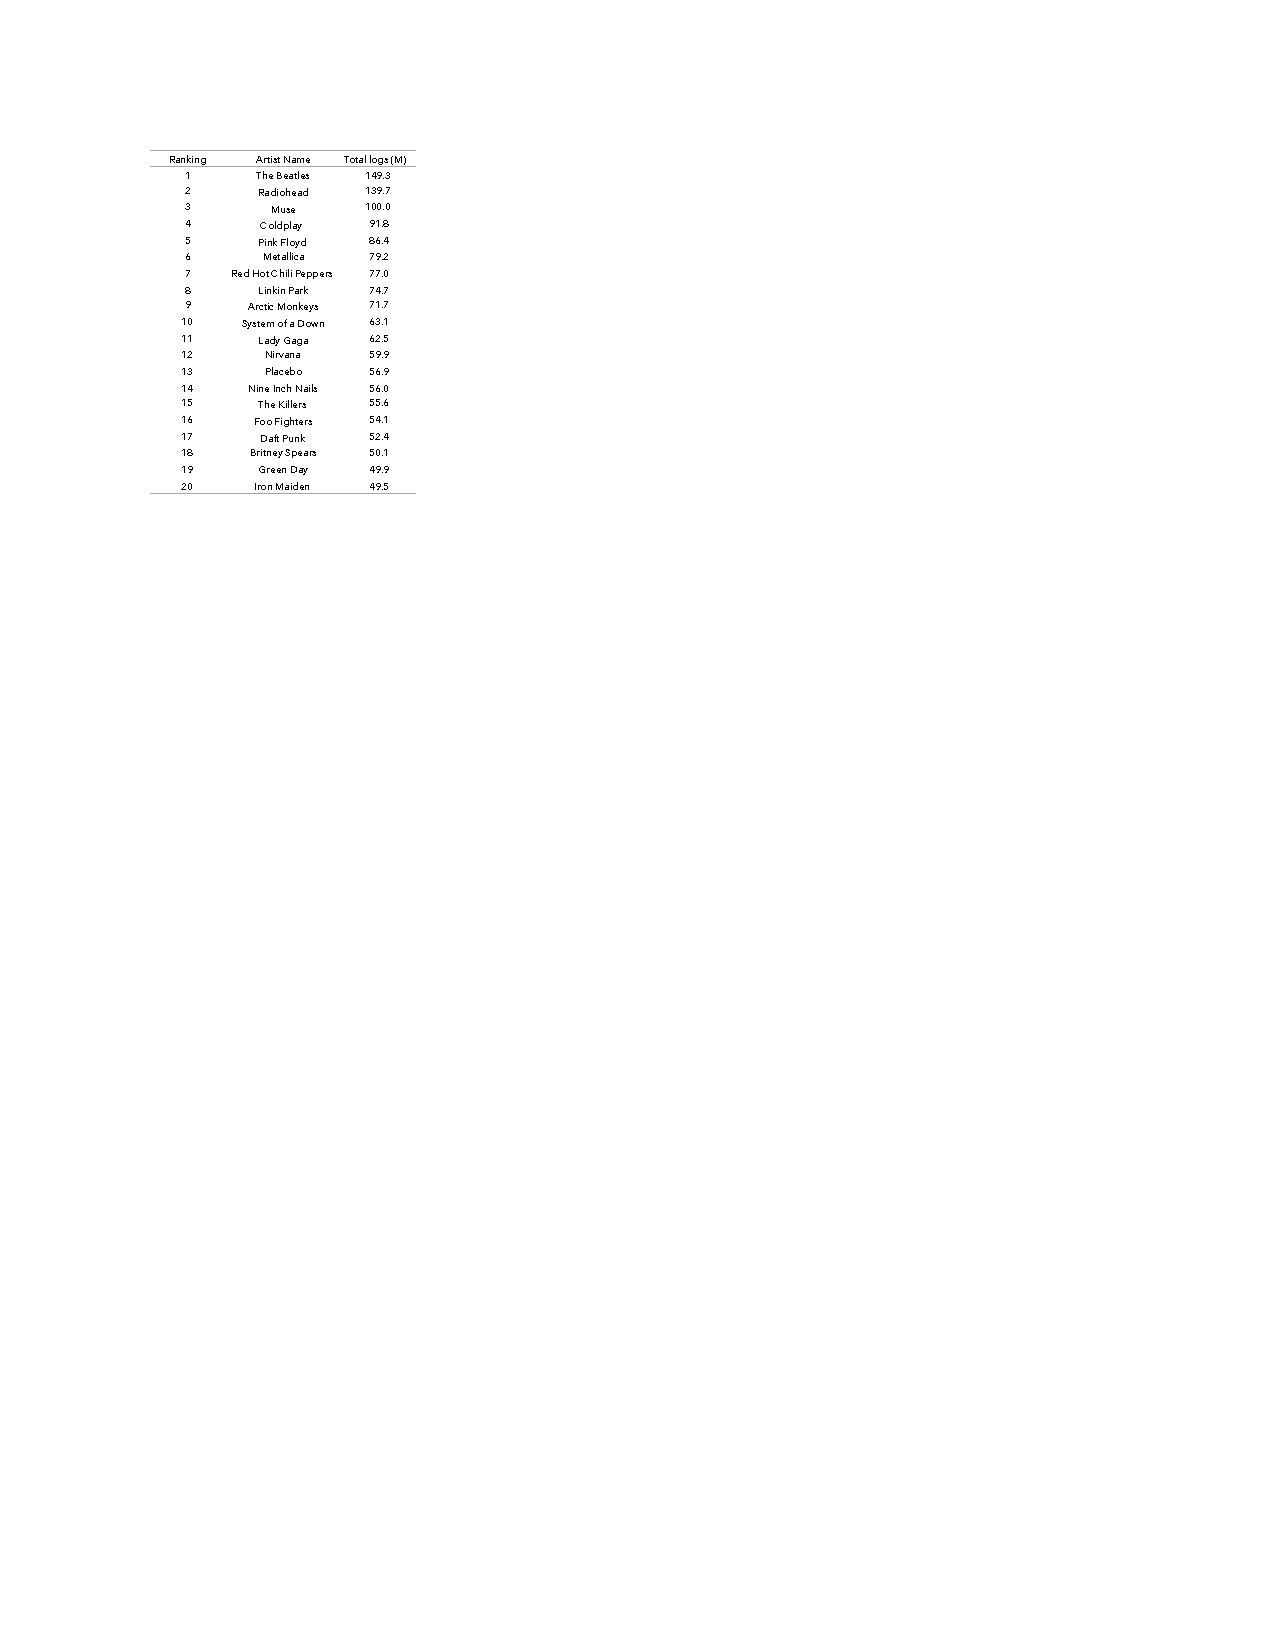
\includegraphics[width = 0.60\textwidth]{ranking_artist_cropped.pdf}

\end{table}

% \newpage
As expected, the first places of the ranking were populated with highly known music artists. However, although there were a number of artists that are considered ``classic'' (e.g., The Beatles or Pink Floyd), several classic music artists were missing in the top 20 positions of the ranking (e.g., Rolling Stones or Michael Jackson). 
% It is also unlikely that users in the MLHD dataset have listened to music artists such as The National more than to Madonna, for example.
Moreover, it is peculiar that all the highly listened artists in the dataset are usually referred to as Pop or Rock artists. There is no representation of other popular genres among young people, such as Electronic or Hip-hop. 
These characteristics of the dataset may indicate that there is a bias in the listeners that are represented in the MLHD dataset. Since the population sample of the dataset is big, we suspect that there is a bias of towards Pop and Rock artists in the Last.fm users. However, we believe that every music streaming service has a specific bias. The Soundcloud music service, for example, is known for being a niche place for Electronic and Hip-hop artists and listeners.





In Table \ref{table:album_ranking} we show the ranking for the 20 most popular albums in the MLHD dataset. 
If the ranking of artists was clearly dominated by very popular artists, the ranking of albums showed a different arrangement. A number of apparently not-so-popular albums occupied the first places of the ranking. 
This characteristic of the ranking of albums in the dataset indicates that the ranking of artists is obviously ranked by the aggregated number of submitted logs for all the releases by an artist. Therefore, music artists with a long and consistent trajectory of good releases reach the first places of the ranking. 
On the other hand, artists with a shorter trajectory or with a few popular releases do not reach the ranking of artists but some of their releases are heavily listened. As a results, they get into the first places of the ranking of albums (e.g., Bon Iver or Paramore).

\graphicspath{{./figs/ch6/}}
\begin{table}[!h]
% \vspace{1em}
\centering
\caption[20 top-ranked albums in the MLHD dataset]{20 top-ranked albums in the MLHD dataset. The ``Total logs'' column refers to the total number of logs, in millions, for the particular albums in the dataset.}\label{table:album_ranking}
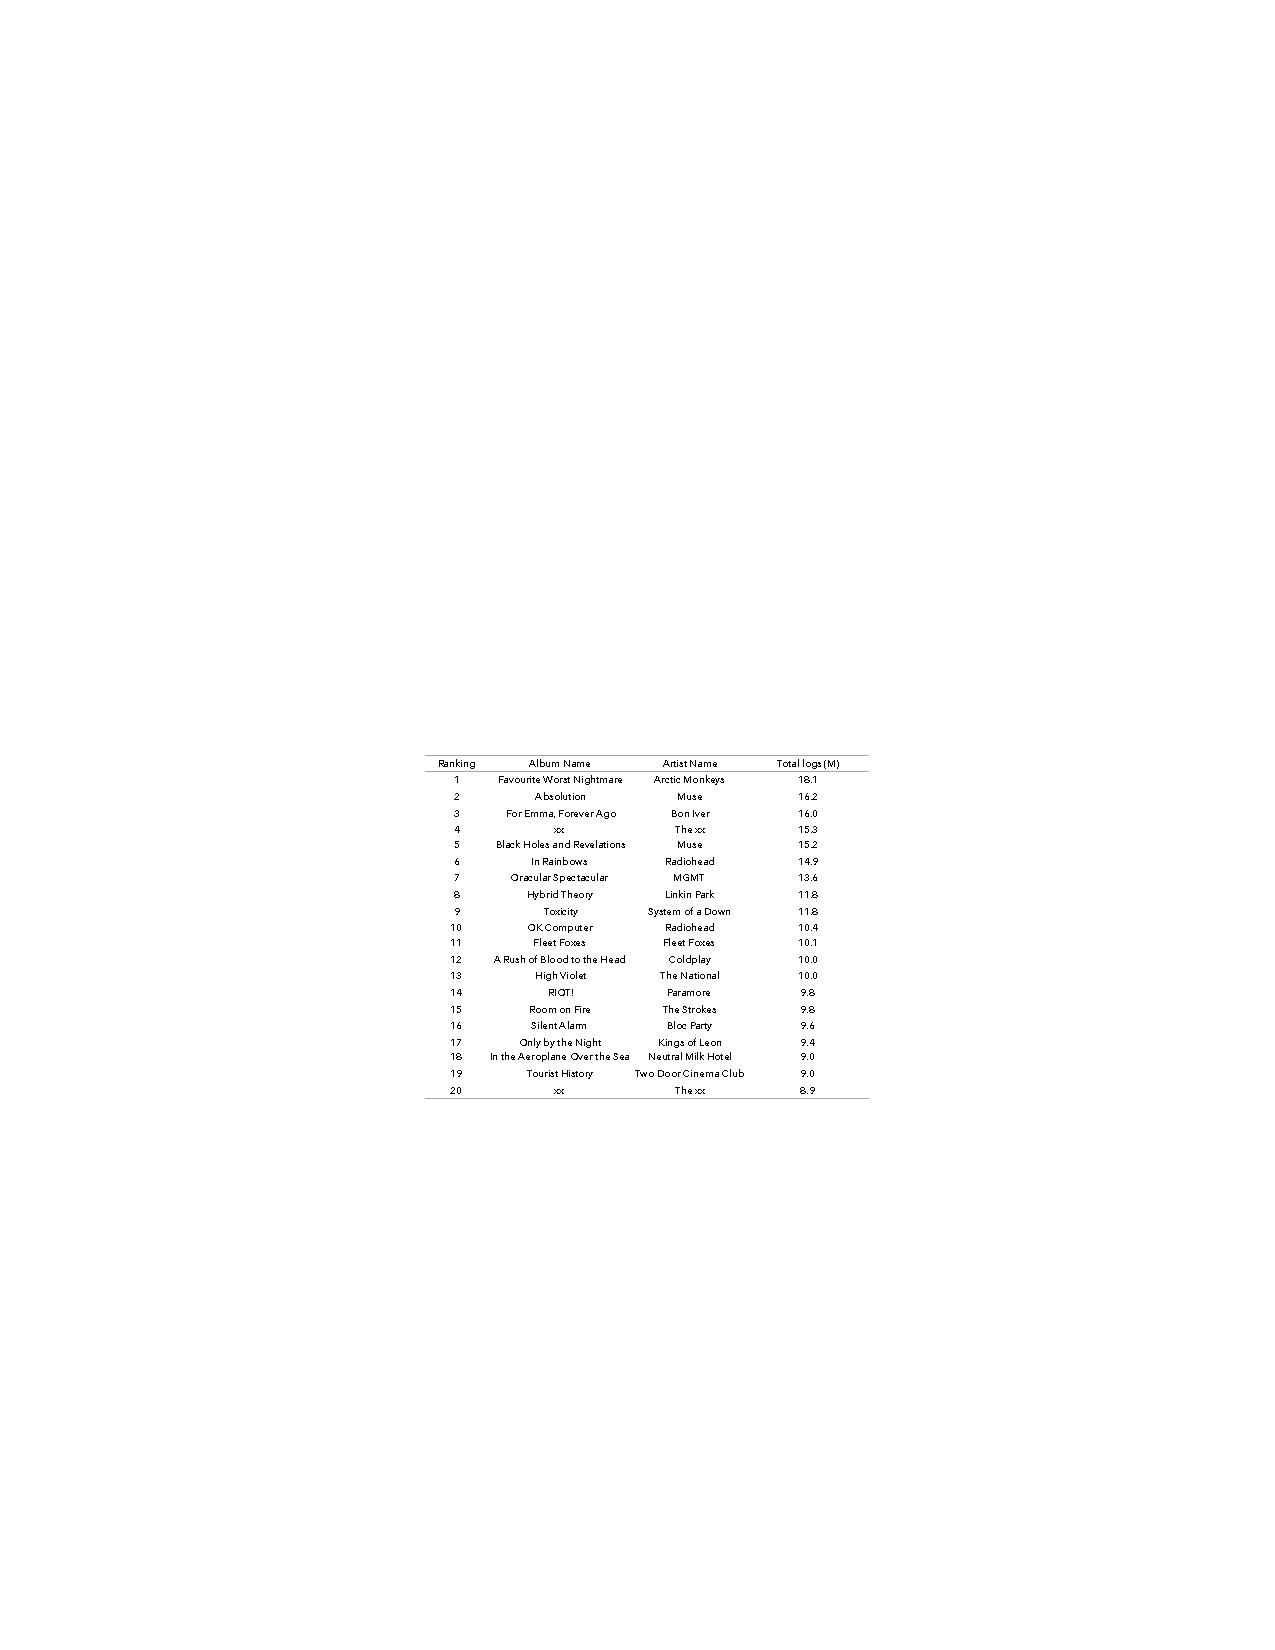
\includegraphics[width = 0.9\textwidth]{ranking_album_cropped.pdf}
\end{table}



It is also interesting to notice that the album ``xx'' by the artist ``The xx'' appears twice in the top 20 ranking. By reviewing this issue closely, we found out that this release appeared at least twice in our dataset, with two different MusicBrainz identifiers (MBIDs) that were not linked to each other.
We reported this issue to Last.fm and MusicBrainz. We did not receive a response from Last.fm, but MusicBrainz replied that some items in their database have  different MBIDs because of processes of merging and splitting. 
For example, if by any reason a user merges the entity Bob Marley with the entity Bob Marley and the Wailers---and this merge is accepted by the MusicBrainz community---the new entity Bob Marley will be reachable by three different MBIDs: the one from the original Bob Marley, the one from Bob Marley and the Wailers, and also from the newly created from the merging process.\footnote{In fact this happened once but the merge was reverted since it was clearly a mistake (\url{https://chatlogs.metabrainz.org/brainzbot/metabrainz/2015-12-04/?msg=3422608&page=1})} 
This behaviour occurs because MusicBrainz do not delete the previous entities, nor their MBIDs, from their database.
MusicBrainz manages to return the latest MBID when someone queries the API with an entity's former MBID by means of redirection tables\footnote{Documentation about the MusicBrainz schema and how redirect tables work is available at \url{https://wiki.musicbrainz.org/MusicBrainz_Database/Schema#Schema}} (e.g., MusicBrainz redirects the MBID used by Last.fm for Britney Spears (\texttt{2f4f5d16-7102-4110-97fd-f5c365d6bb26}) to the latest one on the MusicBrainz database (\texttt{45a663b5-b1cb-4a91-bff6-2bef7bbfdd76})).\linebreak Redirections are not directly available from the MusicBrainz API, but they can be accessed by downloading and using a local copy of the MusicBrainz data\-base.\footnote{Documentation about how to download and set up a local instance of the MusicBrainz database is available at \url{https://musicbrainz.org/doc/MusicBrainz_Database/Download}}
Last.fm, on other hand, does not work with redirections and so they seem to store versions of the same music entity using different MBIDs, and also does not store newly created MBIDs for merged entities.
All in all, if the number of logs of the release ``xx'' by the band ``The xx'' is aggregated, it becomes the most listened album in the dataset. 
% However, for calculating the rankings we did not perform this matching.


 In Table \ref{table:track_ranking} we show the ranking for the 20 most popular tracks in the MLHD dataset. The ranking exhibits a similar behaviour to the ranking of albums, with only a small number of ``classic'' tracks in the first places of the ranking.

\graphicspath{{./figs/ch6/}}
\begin{table}[!h]

\centering
\caption[20 top-ranked tracks in the MLHD dataset]{20 top-ranked tracks in the MLHD dataset. The ``Total logs'' column refers to the total number of logs, in millions, for the particular tracks in the dataset.}\label{table:track_ranking}
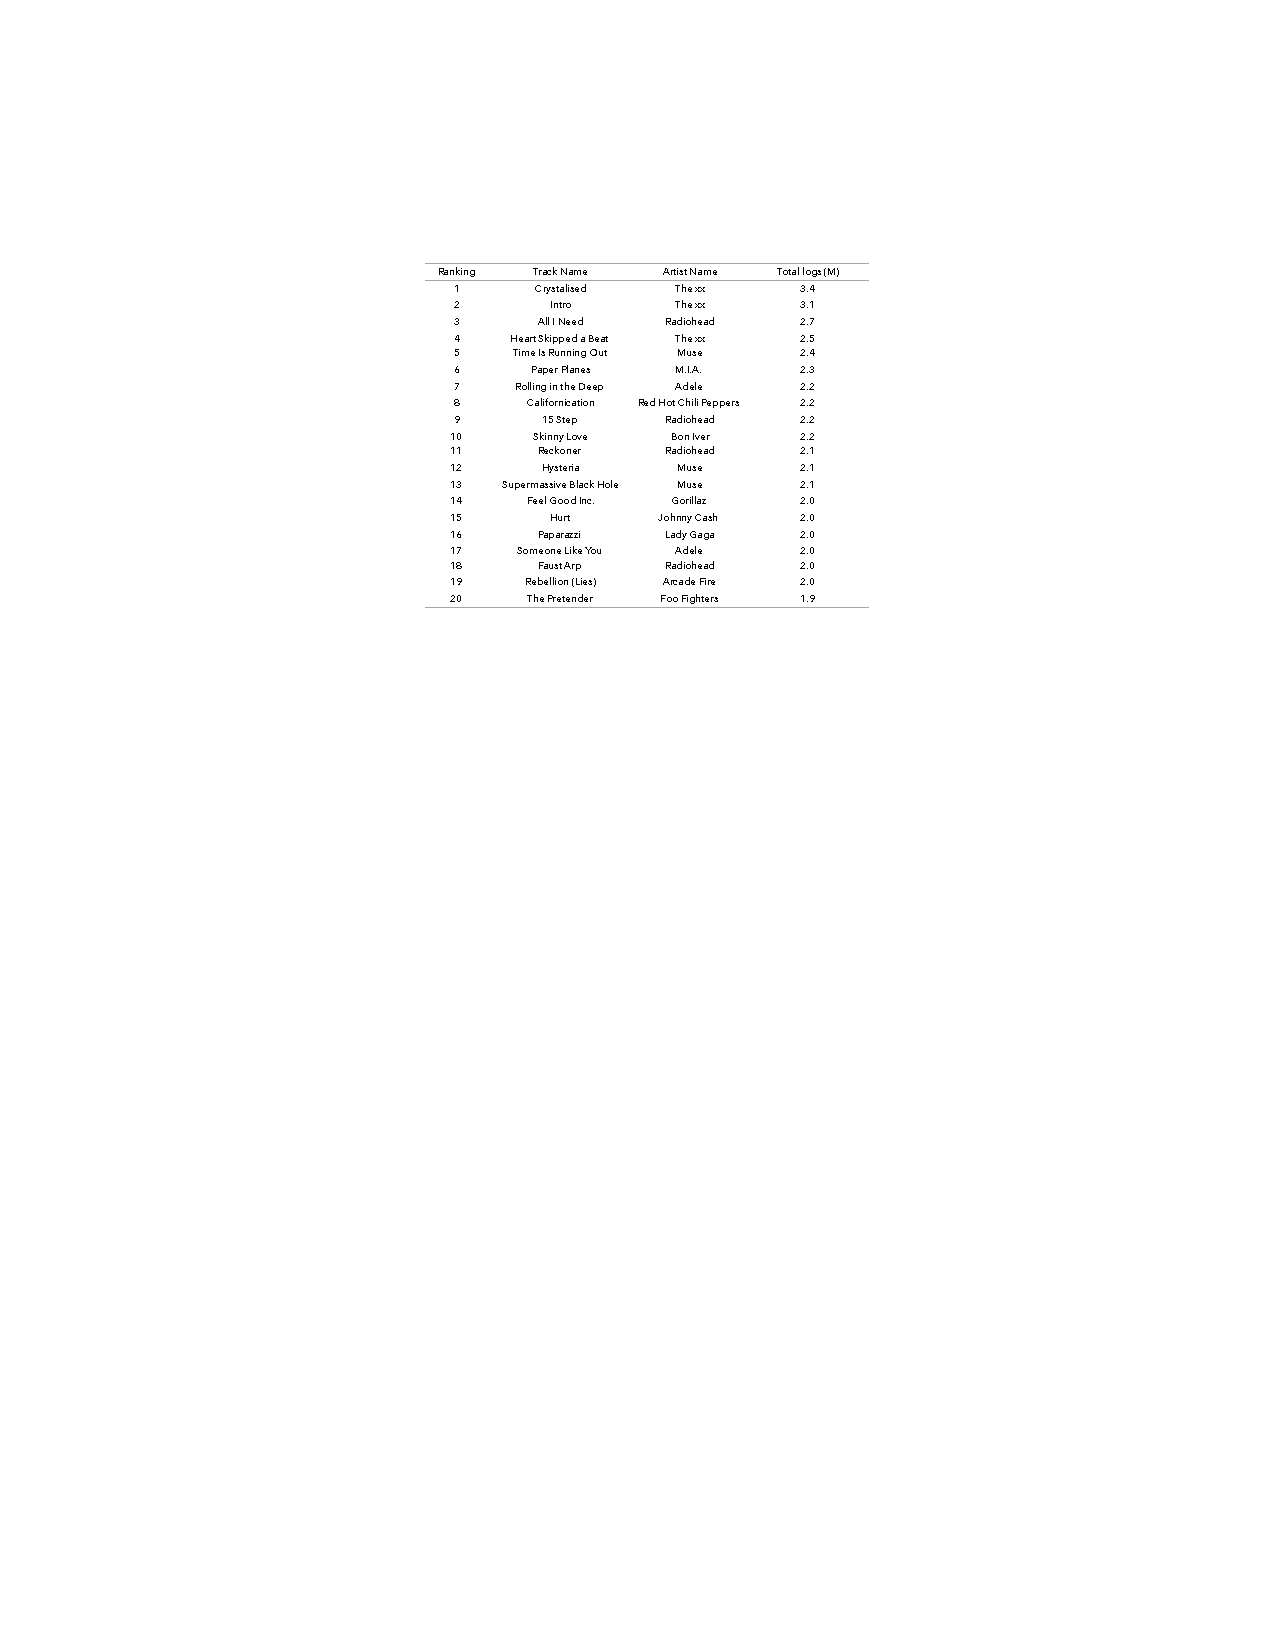
\includegraphics[width = 0.9\textwidth]{ranking_track_cropped.pdf}
\vspace{1em}
\end{table}




\subsubsection{Genderedness}\label{subsec:genderedness}
	With the aim of expressing how close a listener's listening history is to what females or males are listening to, we developed the \emph{genderedness} feature. 
    The genderedness feature computation basically relies on mainstreamness, but instead of computing just one overall ranking from all listeners, it uses two rankings: one made with music logs from listeners self-declared as female, and another one made with music logs from listeners self-declared as male. 

	For each user $x$'s listening history and music item of type $k$, let
	$m_{x,k,male}$ be the mainstreamness computed with the male ranking,
	$m_{x,k,female}$ be the mainstreamness calculated with the female ranking.
   We defined the feature genderedness $g_{x,k}$ for listener $x$ on a given music item of type $k$ as:
          \vspace{1em}
			\begin{equation}
			\abovedisplayskip=2pt plus 3pt minus 9pt
			\label{eq:genderedness}
			g_{x,k}=m_{x,k,male} - m_{x,k,female}
		\end{equation}


\subsubsection{Fringeness}
We developed the \emph{fringeness} feature with the objective of expressing how much a user listened to rare music items. In other words, those items for which the Last.fm database did not have an MBID (see Figure \ref{fig:mbid_combinations_crop} for summary of the percentage of music logs with and without MBIDs for the different music items).

% Let $e_x$ be the number of scrobbles without IDs for music items, and $t_x$ the total number of music logs in the listening history for user $x$, the fringeness value $f_x$ can be expressed as: 
% 	\begin{equation}
% 		\abovedisplayskip=2pt plus 3pt minus 9pt
% 		f_x = \frac{e_x}{t_x}
% 	\end{equation}


	For each user $x$'s listening history, let 
%     $L$ be the number of submitted music logs,
    $S_k$ be all submitted music items of type $k$, where $k$=\{tracks, albums, artists\},
%     $s_i$ be the number of music logs for any given music item key at ranking $i$. 
	$F_k$ be the number of music logs of type $k$ without IDs in the Last.fm database.
    
    We defined the feature fringeness $f_{x,k}$ for listener $x$ on a given music item of type $k$ as:

	\begin{equation}
		\abovedisplayskip=2pt plus 3pt minus 9pt
		f_{x,k} = \frac{F_x}{S_x}
	\end{equation}


% \vspace{0.5cm}












\subsection{Profiling listeners}\label{sec:profiling}
\graphicspath{{./figs/ch6/}}
% Age seems now to be important.
% From \textcite{straw90popular}
% While the programming principles of Top 40 radio have long been regarded as appropriate to an audience dominated by adolescents, Top 40 programmers have, for the most part, conceived that audience in only the most general of demographic terms. Despite the rise of detailed demographic profiles of radio audience since the mid-1960s, Top 40 stations would continue, throughout the 1970s, to regard their adolescent listeners as the active core at the centre of a wider, general audience, rather than as a restricted demographic group with its own, specific appeal to advertisers. This general audience is often seen to be stratified, with, as its core, a group of adolescent listeners active in the monitoring of musical innovation and in the purchasing of musical recordings, but in their competition for advertising revenues Top 40 radio stations will usually identify themselves as having a "mass appeal."
To illustrate how the features we developed can be used to profile listeners, we calculated the exploratoryness, mainstreamness, genderedness, and fringeness for all users in the MLHD dataset,  for each one of the music entities. 
As we saw in Subsection \ref{sub:cleaning}, not all music logs within each listening history had a full set of MBIDs, and so we ended up using the total number of logs that had a MBID for the specific music entity at hand. 
In total, we used 93 percent of logs of the dataset when computing profiling features in relation to artists, 64 percent with albums, and 78 percent with tracks.


In Figure \ref{fig:mainstreamness_by_age} we show a boxplot summary of the calculated mainstreamness values by age, computed for all listeners in our dataset with self-declared age within [15, 54] years old.
We can see in the figure that younger people tend to have higher levels of mainstreamness, disregarding if the music item is an artist, album, or track. 
Since mainstreamness is based on comparing rankings of music items, this characteristic indicates that younger people tend to listen more to music items that are ranked higher in the overall ranking of music items. On the other hand, older people listen to music that is experienced less frequently, in general.
The mainstreamness feature value of all three music items diminishes steadily with age and tends to plateau when people get older.
The three plots in the figure also display an uneven change in the distributions of the computed mainstreamness for the population of listeners in their forties and fifties, as well as for 15-year-old listeners. 
The larger variability in these populations may be explained due to the much smaller number of music listening histories from listeners within those age ranges.

\graphicspath{{./figs/ch6/}}
\begin{figure}[!t]
	\centering
	\begin{subfigure}[b]{\textwidth}
		\centering
		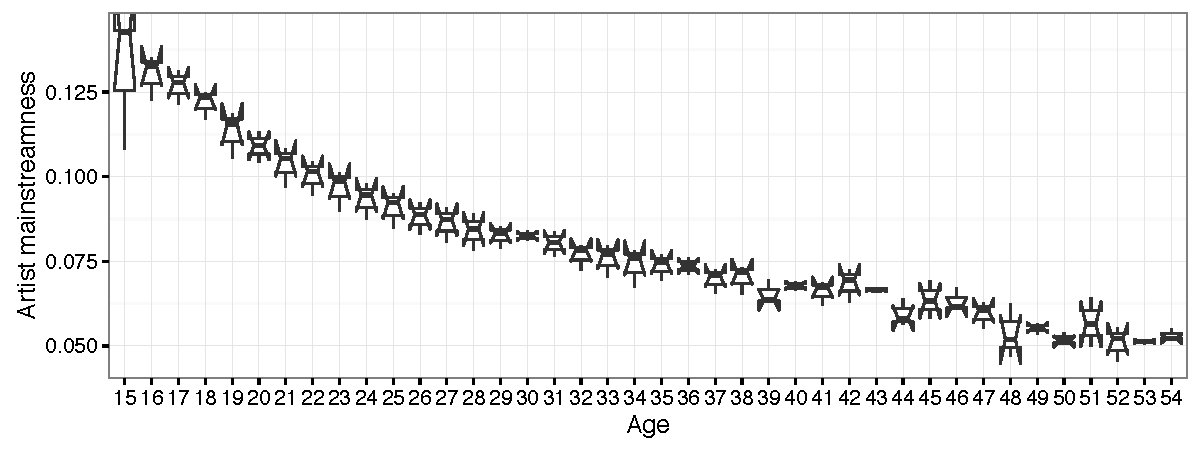
\includegraphics[width=0.75\textwidth]{artist_mainstreamness.pdf}
        \caption{Artist mainstreamness by age}
        \label{fig:artist_mainstreamness}
	\end{subfigure}
    % \vspace{5pt}

	\begin{subfigure}[b]{\textwidth}
		\centering
		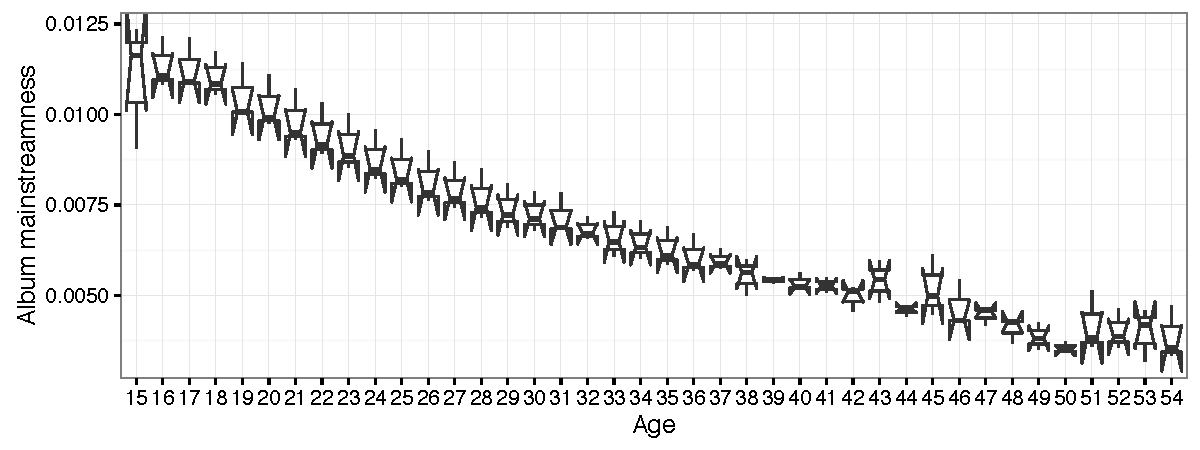
\includegraphics[width=0.75\textwidth]{album_mainstreamness.pdf}
        \caption{Album mainstreamness by age}
        \label{fig:album_mainstreamness}
	\end{subfigure}
    % \vspace{5pt}

	\begin{subfigure}[b]{\textwidth}
		\centering
		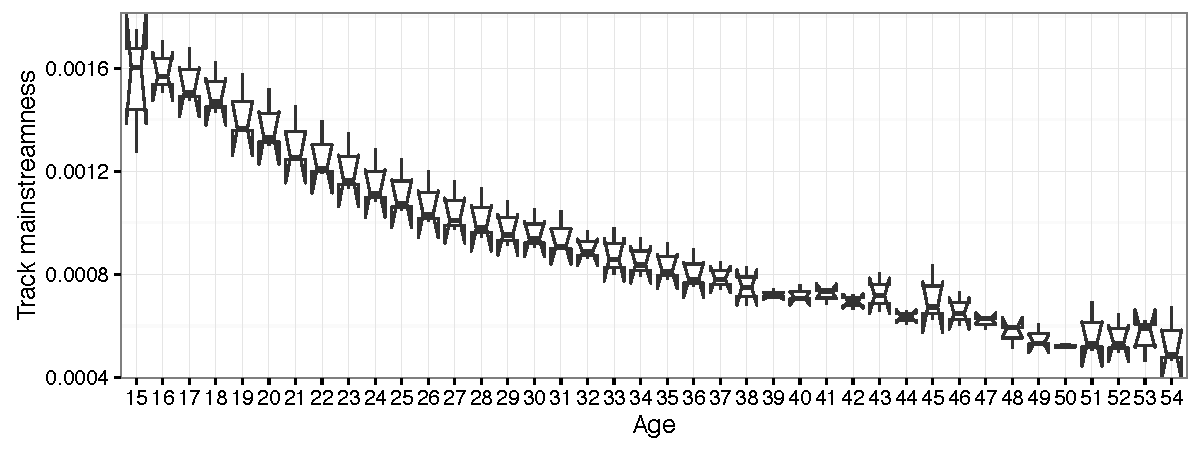
\includegraphics[width=0.75\textwidth]{track_mainstreamness.pdf}
        \caption{Track mainstreamness by age}
        \label{fig:track_mainstreamness}
	\end{subfigure}
    % \vspace{10pt}
	\caption[Summary of computed artist, album, and track mainstreamness]{Boxplots showing summary of the calculated artist, album, and track mainstreamness values by listeners' age, computed for all users in MLHD with a self-declared age within [15, 54] years old.}
	\label{fig:mainstreamness_by_age}
\end{figure}

% Boxplots are a summarised visual representation of batches of data. The central, horizontal line within each boxplot shows the median. The first and third quartiles (i.e., the 25th and 75th percentiles) are shown by lower and upper hinges. The extremes show about 99 percent of the total amount of the data distribution. Finally, the notches surrounding the median show a measure of the significance of the differences between the populations. If the notches do not overlap, the medians are significantly different at 95 percent confidence level \autocite{mcgill78variations}. 






We have to note that, since mainstreamness is defined based on the ranking of the music items in the whole dataset, the distribution of mainstreamness across age could be affected by the fact that the dataset is dominated by younger users. However, the mainstreamness feature tries to express the degree of similarity of a listener's history to what everyone else listened to, and so this behaviour is expected, particularly if the dataset population is biased towards a specific group.

\begin{figure}[!t]
	\centering
	\begin{subfigure}[b]{\textwidth}
		\centering
		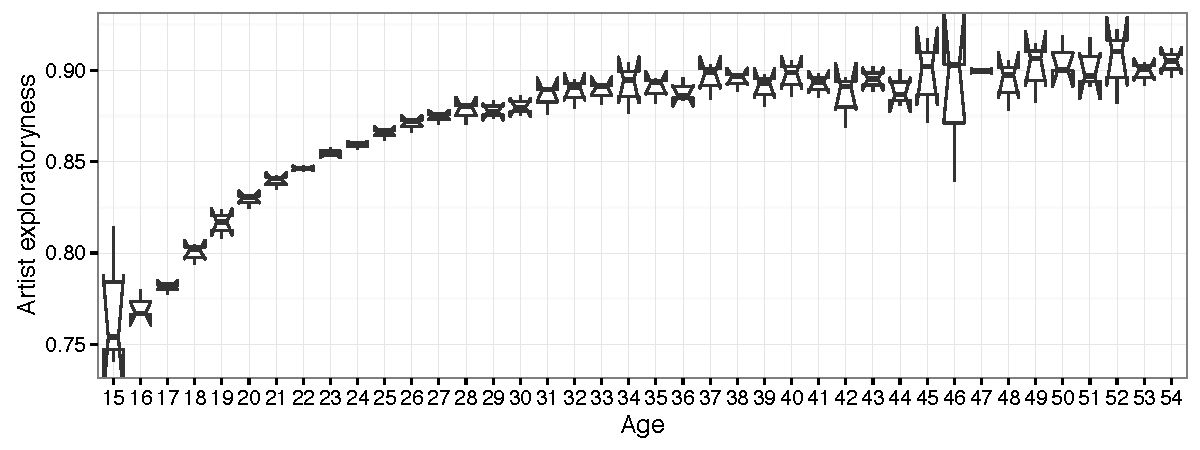
\includegraphics[width=0.75\textwidth]{artist_exploratoryness.pdf}
        \caption{Artist exploratoryness by age}
        \label{fig:artist_exploratoryness}
	\end{subfigure}
    % \vspace{10pt}

	\begin{subfigure}[b]{\textwidth}
		\centering
		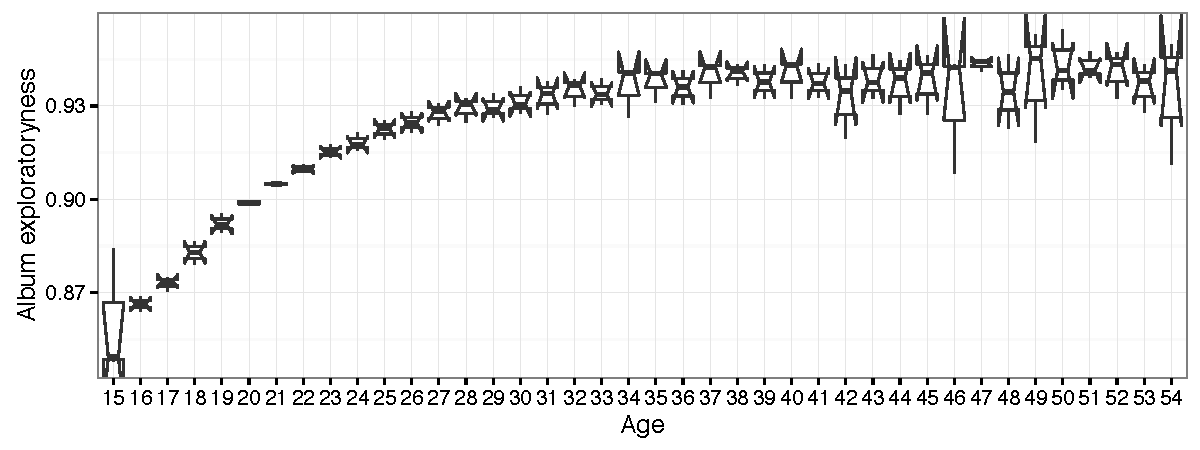
\includegraphics[width=0.75\textwidth]{album_exploratoryness.pdf}
        \caption{Album exploratoryness by age}
        \label{fig:album_exploratoryness}
	\end{subfigure}
    % \vspace{10pt}

	\begin{subfigure}[b]{\textwidth}
		\centering
		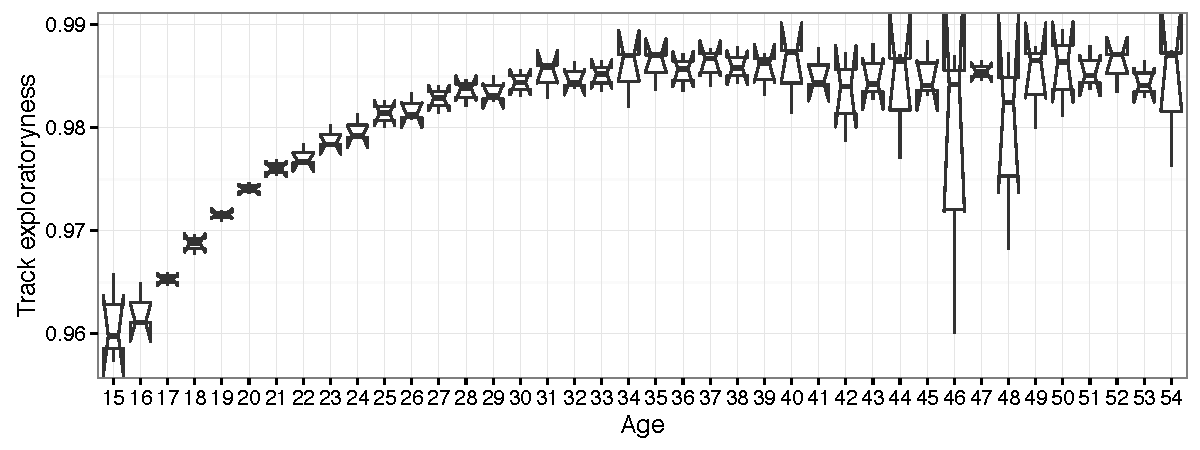
\includegraphics[width=0.75\textwidth]{track_exploratoryness.pdf}
        \caption{Track exploratoryness by age}
        \label{fig:track_exploratoryness}
	\end{subfigure}
    % \vspace{10pt}

\caption[Summary of computed artist, album, and track exploratoryness]{Boxplots summaries of the artist, album, and track exploratoryness by listeners' age, computed for all users in the MLHD with a self-declared age within [15, 54] years old.}
\label{fig:exploratoryness_by_age}
\end{figure}



The computed exploratoryness feature by age of listeners for artists, albums, and tracks is shown in Figure \ref{fig:exploratoryness_by_age}. The boxplots show that there is an increase in the exploratoryness of listeners for all music items while in their late teens and early twenties. This rise tends to plateau for young adults at about 30 years old. 
The variability in the medians increase for older people since the number of music listening histories is much smaller than for younger people, except for 15-year-old listeners.
Although the absolute values of exploratoryness are different for each music item, the shape of the increase in the population curves per age are similar, implying that the relation between exploratoryness and age is the same.
This characteristic seems to indicate that younger people tend to listen to the same music more repeatedly compared with older people. On the other hand, older listeners in the MLHD, listened to artists, albums, and tracks in a more diverse fashion, exploring more items. 


\graphicspath{{./figs/ch6/}}
\begin{figure}[!t]
	\centering
	\begin{subfigure}[b]{\textwidth}
		\centering
		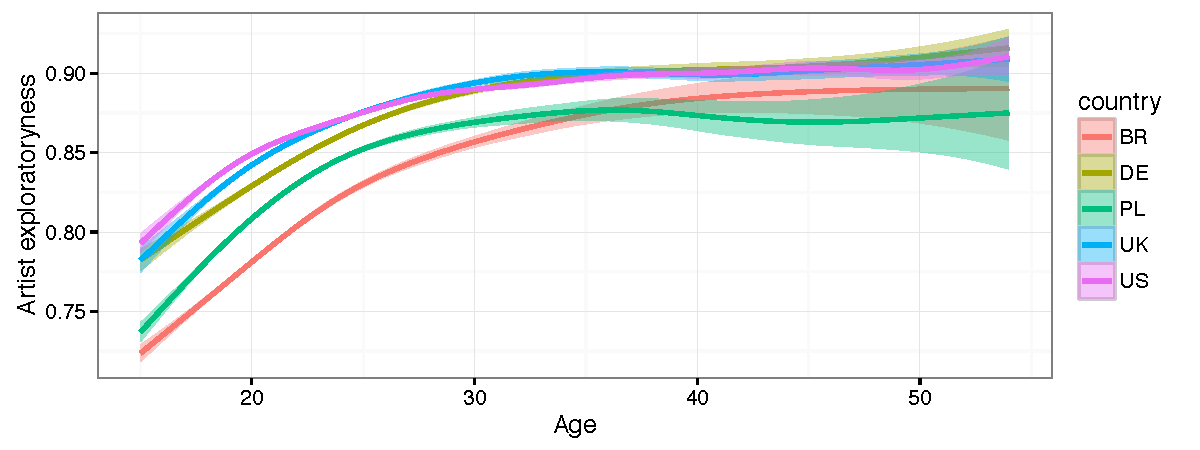
\includegraphics[width=0.66\textwidth]{artist_exploratoryness_by_country.pdf}
        \caption{Artist exploratoryness by age and country of listeners}
        \label{fig:artist_exploratoryness_by_age_and_gender}
	\end{subfigure}
%     \vspace{10pt}

	\begin{subfigure}[b]{\textwidth}
		\centering
		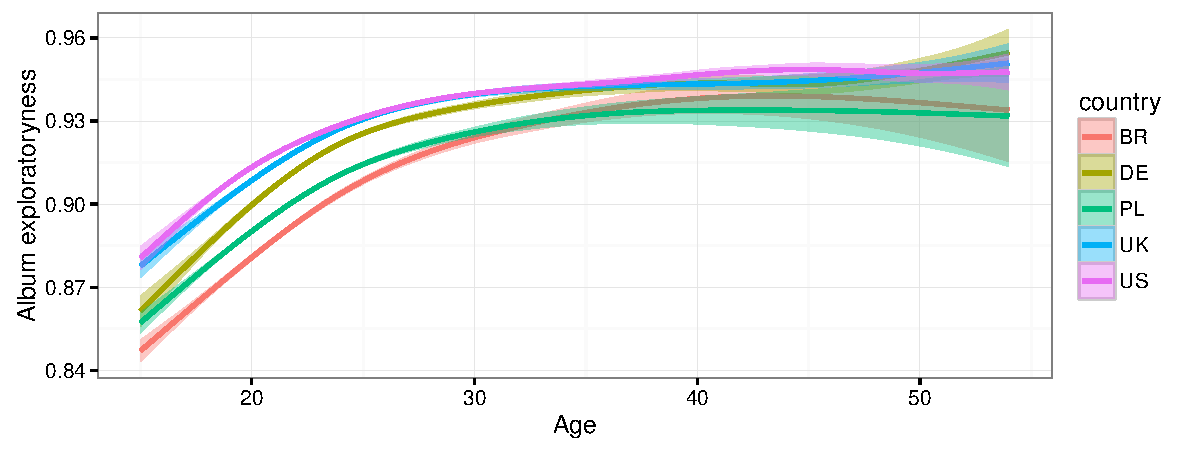
\includegraphics[width=0.66\textwidth]{album_exploratoryness_by_country.pdf}
        \caption{Album exploratoryness by age and country of listeners}
        \label{fig:album_exploratoryness_by_age_and_gender}
	\end{subfigure}
%     \vspace{10pt}

	\begin{subfigure}[b]{\textwidth}
		\centering
		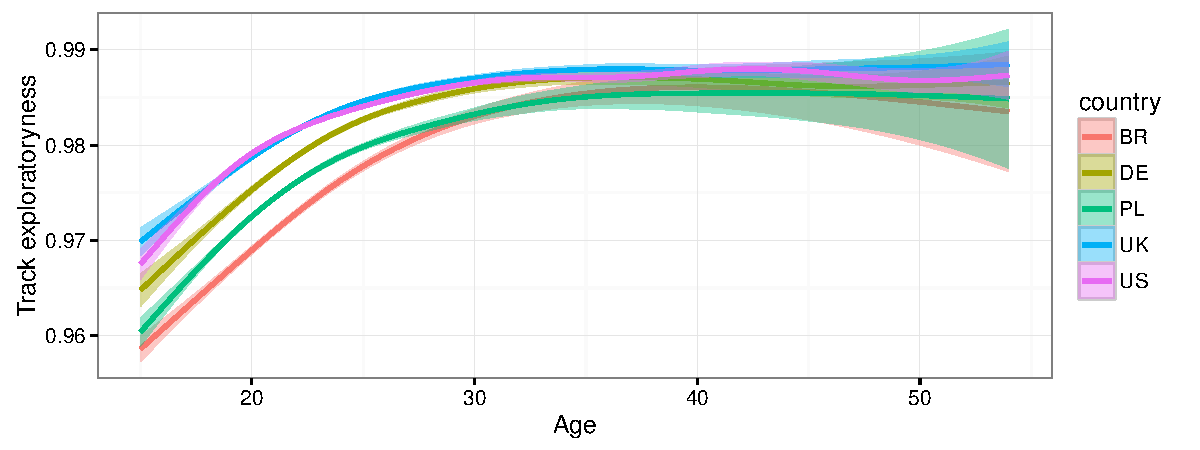
\includegraphics[width=0.66\textwidth]{track_exploratoryness_by_country.pdf}
        \caption{Track exploratoryness by age and country of listeners}
        \label{fig:track_exploratoryness_by_age_and_gender}
	\end{subfigure}
%     \vspace{10pt}

\caption[Artist, album, and track exploratoryness means versus age of listeners]{Exploratoryness mean for artist, album, and track entities in relation to the age of listeners from the five countries with the largest number of listeners in the dataset. Ribbon bands show 95 percent CI bars.}
\label{fig:artist_exploratoryness_by_country}
\end{figure}





% Exploratoryness and five countries
We also verified if the exploratoryness of listeners varied by their country and age. In Figure \ref{fig:artist_exploratoryness_by_country} we show exploratoryness by age for listeners from the five countries with the largest population in the dataset, for the three music items. Ribbon bands show 95 percent confidence interval bars.
The curves of exploratoryness show a similar trend in terms of age to the previous figure. However, if we analyse them by country, we can observe that while people from the US and UK have similar levels of exploratoryness across all ages for the three music items, young users from DE (Germany) in their late teens and early twenties are less exploratory. However, Germans in their thirties and onwards reach a similar level of exploratoryness as that of anglophones. Listeners from PL (Poland) and BR (Brazil) are consistently less  exploratory than people from the previously mentioned countries, but especially youths and young adults.

% Exploratoryness and gender
In order to visualise if there were any trends in terms of exploratoryness and self-declared gender and age, in Figure \ref{fig:exploratoryness_by_gender} we show exploratoryness means and 95 percent confidence interval bands for all music items. 
\graphicspath{{./figs/ch6/}}
\begin{figure}[!h]
	\centering
	\begin{subfigure}[b]{\textwidth}
		\centering
		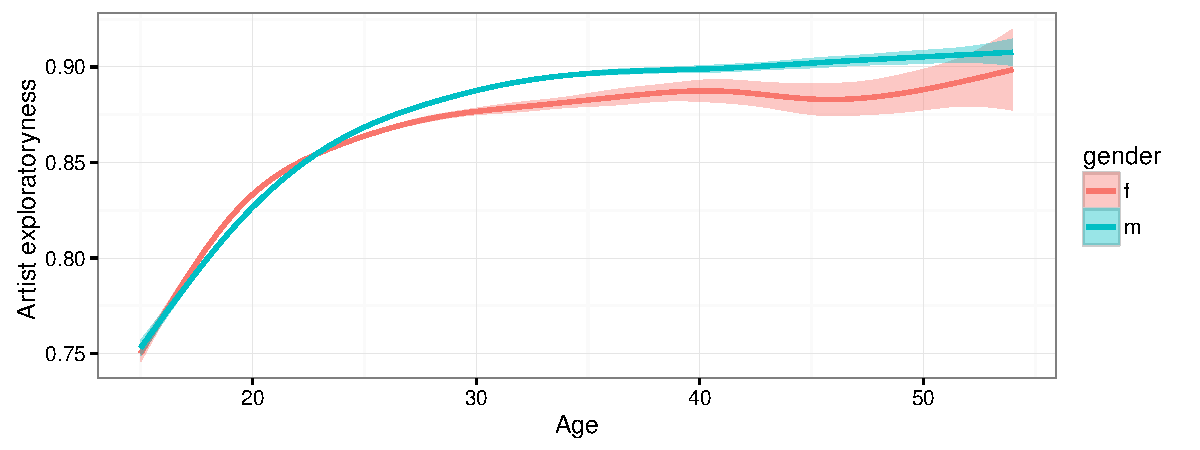
\includegraphics[width=0.75\textwidth]{artist_exploratoryness_by_age.pdf}
        \caption{Artist exploratoryness by age and gender}
        \label{fig:artist_exploratoryness_by_age}
	\end{subfigure}
    % \vspace{10pt}

	\begin{subfigure}[b]{\textwidth}
		\centering
		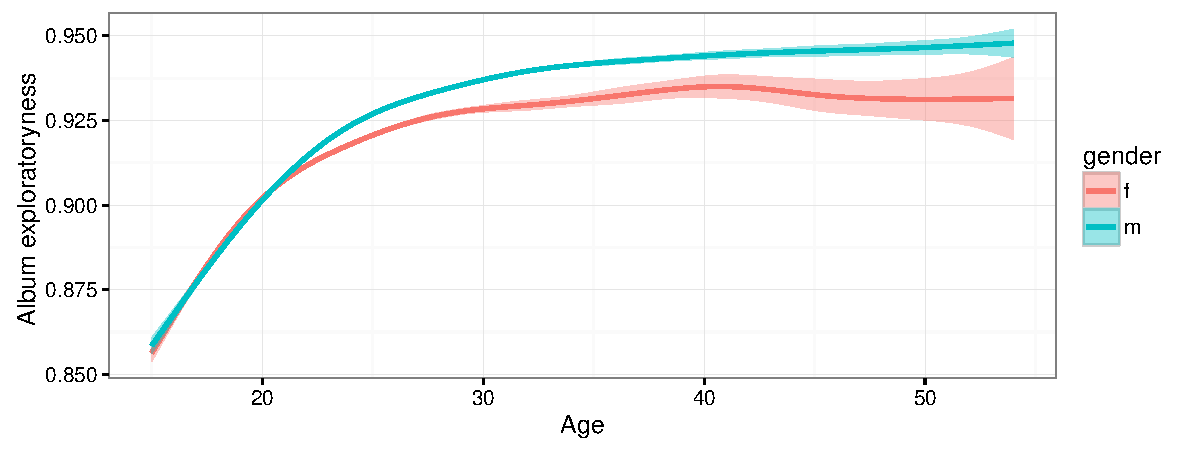
\includegraphics[width=0.75\textwidth]{album_exploratoryness_by_age.pdf}
        \caption{Album exploratoryness by age and gender}
        \label{fig:album_exploratoryness_by_age}
	\end{subfigure}
    % \vspace{10pt}

	\begin{subfigure}[b]{\textwidth}
		\centering
		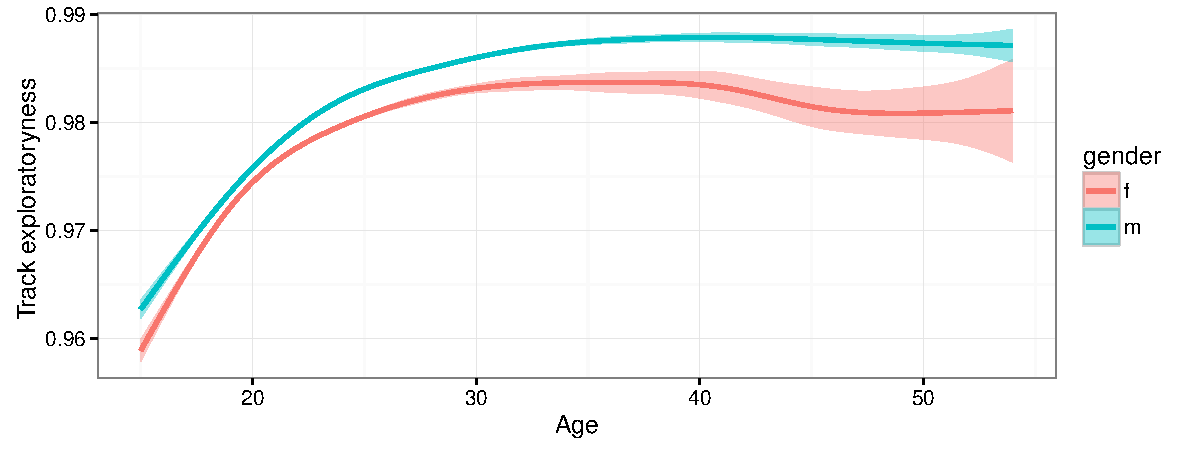
\includegraphics[width=0.75\textwidth]{track_exploratoryness_by_age.pdf}
        \caption{Track exploratoryness by age and gender}
        \label{fig:track_exploratoryness_by_age}
	\end{subfigure}
    % \vspace{10pt}
\caption[Exploratoryness mean by age and gender of listeners]{Exploratoryness mean by age and gender of listeners. Ribbon bands show 95 percent CI bars.}
\label{fig:exploratoryness_by_gender}
\end{figure}

The curves show that, in general, young female and male listeners had similar levels of exploratoryness, in particular for artists  (Fig. \ref{fig:artist_exploratoryness_by_age}) and albums (Fig. \ref{fig:album_exploratoryness_by_age}). However, young adult and adult males become more exploratory than females in regard to those music items. Males exhibit a higher exploratoryness for track throughout all age groups (Fig. \ref{fig:track_exploratoryness_by_age}).





% We can observe from the previous plots that, in general, similar trends can be found for any of the three music items. Because of this, unless we specifically mention it, we will show the relation of subsequent features only in regards to the music item of \textit{artists}.

% Fringeness, gender and age
We also computed fringeness in relation to the self-declared gender and age  of listeners. As we can see in Figure \ref{fig:fringeness_by_gender}, listeners exhibited some differences in terms of fringeness, particularly in relation to their self-declared gender. 
Overall, users within our dataset self-declared as male listened more than female to fringe music items---those items that were not part of the Last.fm database at the moment of the data collection. Artist fringeness (Fig. \ref{fig:artist_fringeness_by_age}) and track fringeness (Fig. \ref{fig:track_fringeness_by_age}) was consistently larger for males across all ages, except for the youngest listeners. Instead, listeners of both genders had similar means for album fringeness, especially in their late twenties and early thirties (Fig. \ref{fig:album_fringeness_by_age}).

\graphicspath{{./figs/ch6/}}
\begin{figure}[!t]
	\centering
	\begin{subfigure}[b]{\textwidth}
		\centering
		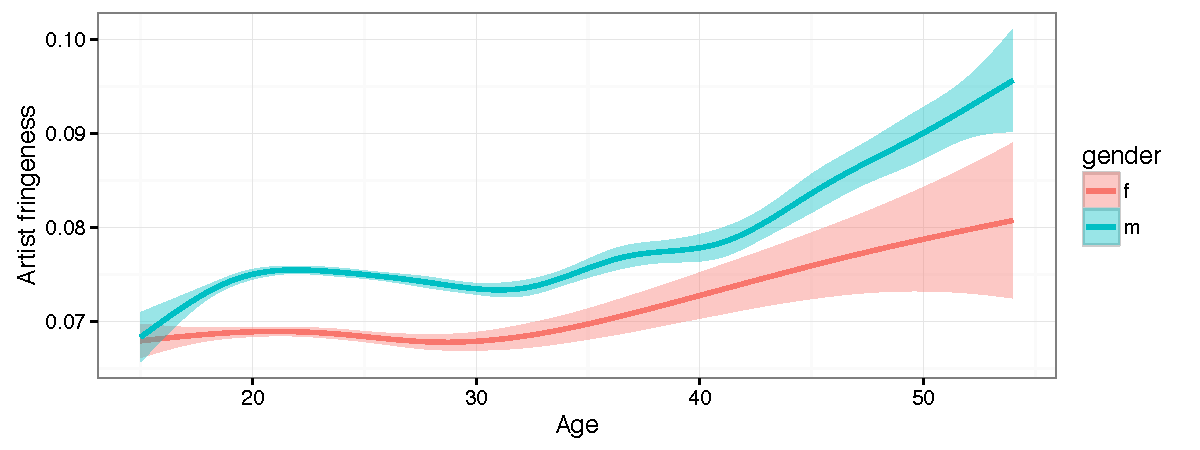
\includegraphics[width=0.75\textwidth]{artist_fringeness_by_gender.pdf}
        \caption{Artist fringeness by age and gender}
        \label{fig:artist_fringeness_by_age}
	\end{subfigure}
    % \vspace{10pt}

	\begin{subfigure}[b]{\textwidth}
		\centering
		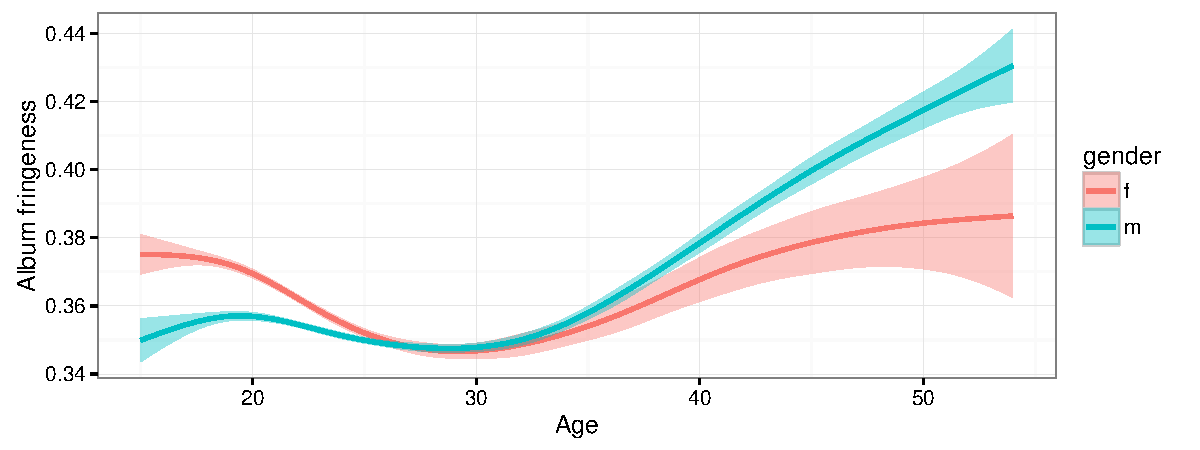
\includegraphics[width=0.75\textwidth]{album_fringeness_by_age_and_gender.pdf}
        \caption{Album fringeness by age and gender}
        \label{fig:album_fringeness_by_age}
	\end{subfigure}
    % \vspace{10pt}

	\begin{subfigure}[b]{\textwidth}
		\centering
		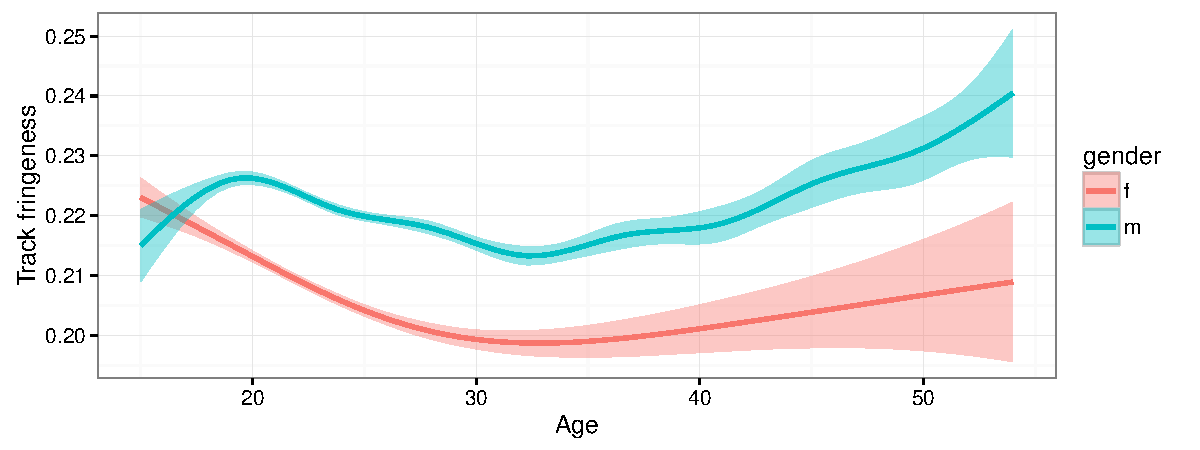
\includegraphics[width=0.75\textwidth]{track_fringeness_by_age_and_gender.pdf}
        \caption{Track fringeness by age and gender}
        \label{fig:track_fringeness_by_age}
	\end{subfigure}
    % \vspace{10pt}

\caption[Fringeness mean by age and gender of listeners]{Fringeness mean by age and gender of listeners. Ribbon bands show 95 percent CI bars.}
\label{fig:fringeness_by_gender}
\end{figure}



We also found differences in regard to artist fringeness by countries. In Figure \ref{fig:artist_fringeness_by_country} we show boxplots of the artist fringeness for listeners from the top 19 countries---those countries whose number of listeners was at least one percent of the total number of listener in the dataset.
Three countries exhibited significant differences in terms of artist fringeness. These countries were JP (Japan), RU (Russia), and UA (Ukraine).
We hypothesised that this trend may be due to (i) people in those countries simply listen more to artists that are not in the Last.fm database, or (ii) they use their own alphabet (e.g., Cyrillic and Katakana) in the metadata on their digital music devices. Therefore, when they submit a music log with those characters there is no probability of finding a match in the Last.fm database. Unlike MusicBrainz, which is designed to support multiple languages,\footnote{MusicBrainz internationalization and multiple language support documentations is available at \url{https://musicbrainz.org/doc/Internationalization}} the Last.fm API only supports English. 


\graphicspath{{./figs/ch6/}}
\begin{figure}[tbp]
% \vspace{1em}
\centering
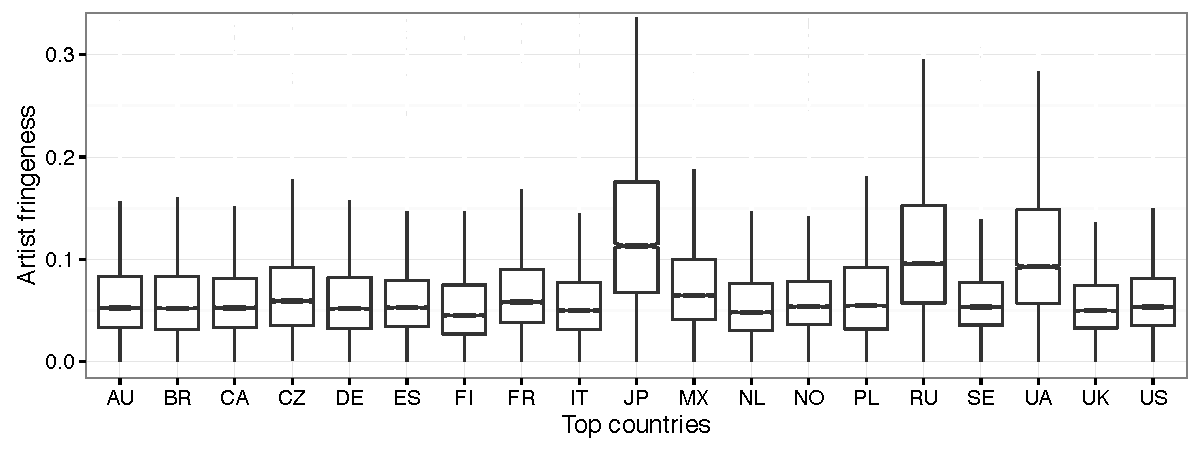
\includegraphics[width = 0.9\textwidth]{artist_fringeness_by_country.pdf}
\caption[Summary of artist fringeness by age and country of listeners]{Boxplot summary of artist fringeness by age and country of listeners. Only Japan (JP), Russia (RU), and Ukraine (UA) exhibit a significant difference.}
\label{fig:artist_fringeness_by_country}
\end{figure}





In regard to fringeness and age, instead of comparing one specific age number with the next, or the previous one, we also compared age groups (e.g., youth versus older listeners).
Therefore, in order to make a proper comparison that does not violate the assumption of homogeneity of variance, we grouped listeners into four groups: 15--24, 25--34, 35--44, and 45--54, and we balanced the number of samples within each of those groups.
We calculated the number of listeners for each age within the age range [15, 54] and observed that the minimum value was 211 for the 54-year-old listeners. 
In order to obtain balanced groups, we decided to draw a random sample of 200 people from each age and we created five 10year groups. As a result, we ended up with 2K listeners in each of the age groups.
% We then bootstrapped these groups with 1000 replications of the original sample.

We performed a similar feature computation to the one that we did before but instead of using the whole population, we used the balanced groups. Visualizing summaries with population groups of the same size would allow us to know if the trends we found from previous analyses were similar.  
% Instead of repeating all processes, from now onwards we will only show the summary of the profiling features in regards to artists and the age group of listeners, since its interaction was most significant.
Although we quantified these characteristics of listeners in relation to artists, albums, and tracks, and their interaction with listeners' age group, the interaction with artists seemed the largest. Therefore, instead of showing all interactions, we will henceforth only show the summary of the profiling features related to artists and the age group of listeners, since that interaction was significant and had a larger effect size.
In Figure \ref{fig:artist_profiling_features_age_groups} we show boxplot summaries for artist mainstreamness, exploratoryness, and fringeness by age groups. 

% N=211 people (54 years old)
% N=20 females (53 years old)

\begin{figure}[!h]
	\centering
	\begin{subfigure}[h]{\textwidth}
		\centering
		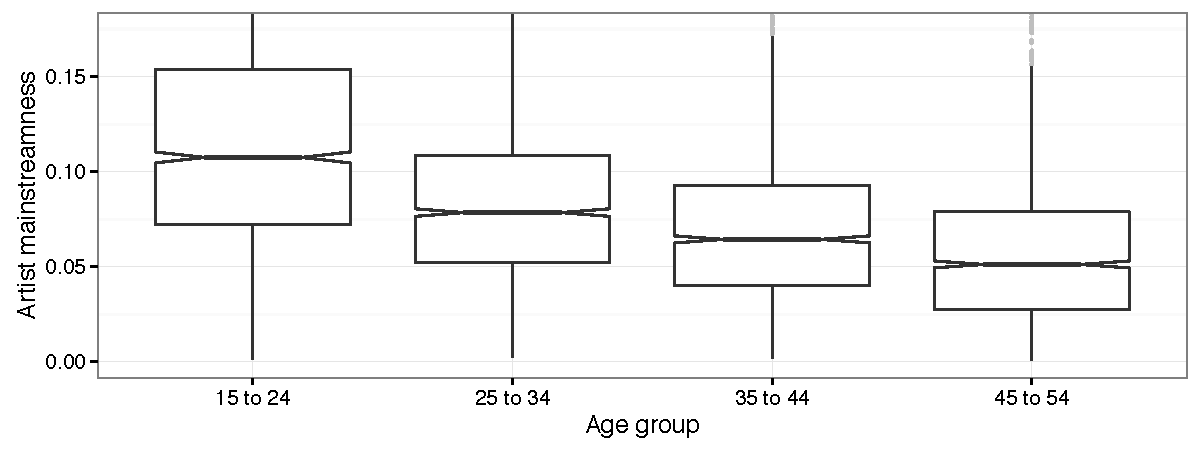
\includegraphics[width=0.75\textwidth]{artist_mainstreamness_by_age_groups_boxplot.pdf}
        \caption{Artist mainstreamness by age group}
        \label{fig:artist_mainstreamness_by_age_groups_boxplot}
	\end{subfigure}
    % \vspace{10pt}

	\begin{subfigure}[h]{\textwidth}
		\centering
		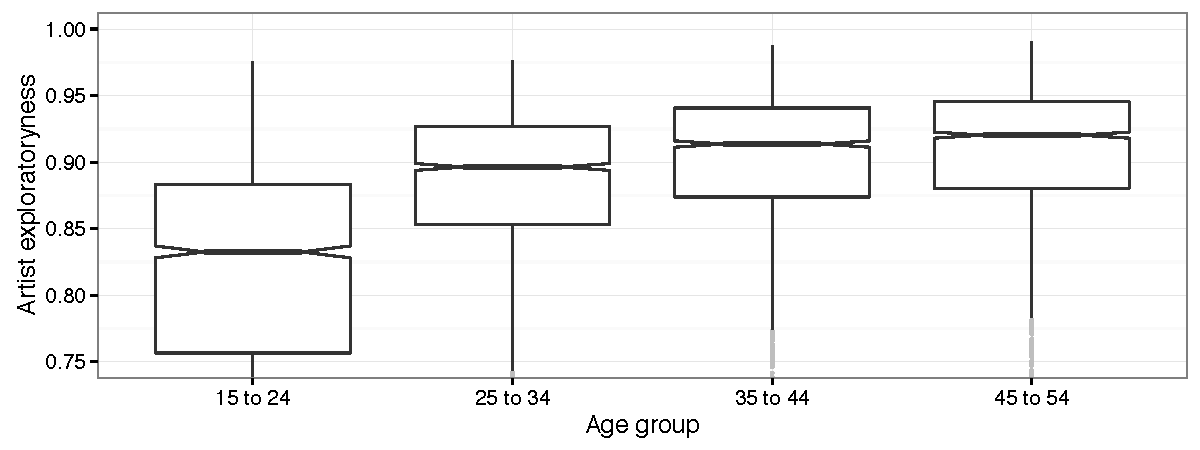
\includegraphics[width=0.75\textwidth]{artist_exploratoryness_by_age_groups_boxplot.pdf}
        \caption{Artist exploratoryness by age group}
 		\label{fig:artist_exploratoryness_by_age_groups_boxplot}
	\end{subfigure}
    % \vspace{10pt}

	\begin{subfigure}[h]{\textwidth}
		\centering
		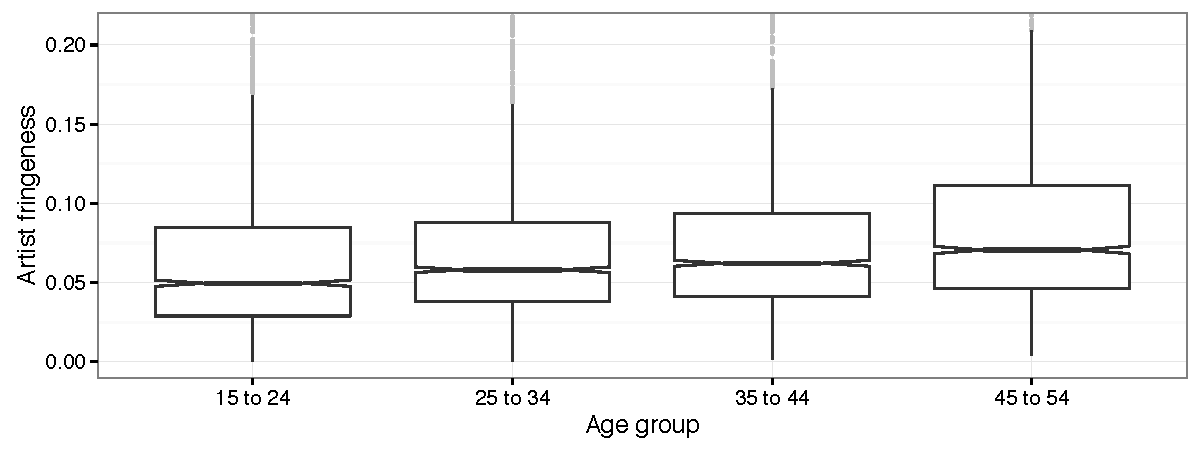
\includegraphics[width=0.75\textwidth]{artist_fringeness_by_age_groups_boxplot.pdf}
        \caption{Artist fringeness by age group}
        \label{fig:artist_fringeness_by_age_groups_boxplot}
	\end{subfigure}
    % \vspace{10pt}

\caption[Summary of artist mainstreamness, exploratoryness and fringeness by age groups]{Summary of the calculated artist mainstreamness, exploratoryness and fringeness values by age groups for a random group of listeners from the MLHD. Each age group size was balanced (N = 2K).}
\label{fig:artist_profiling_features_age_groups}
\end{figure}




In terms of artist mainstreamness, we can see in  Figure \ref{fig:artist_mainstreamness_by_age_groups_boxplot} that, since the notches of the boxplots did not overlap, the feature medians differ.
This means that while younger people listened more to the same artists that everyone was listening to, older people tended to listen to less common performers. 
This effect could be generated by the actual listening behaviour of older people that listened less to highly ranked artists, or because they listened to artists from other eras that were lower in the ranking, or because there were fewer older people in the original dataset and so the artists they listened to were ranked lower in the overall ranking. 
The largest median difference was between the first age group (i.e., 15 to 24 years old) and the second one (i.e., 25 to 34). For older listeners, the  differences between their age groups medians were still significant, but they tended to be smaller.  

In Figure \ref{fig:artist_exploratoryness_by_age_groups_boxplot} we see a boxplot summary of artist exploratoryness. It shows that while listeners of the first group tended to listen over and over to the same artists, more than people from the other groups, listeners from the older age groups tended to explore more artists. The rise in artist exploratoryness gradually decreased, and the medians for the third (i.e., 35 to 44 years old) and fourth group (i.e., 45 to 54) were closer than between the other age groups.

The artist fringeness summary by age group is shown in the boxplot summary in  Figure \ref{fig:artist_fringeness_by_age_groups_boxplot}. We can see that  listeners in the older age groups tended to listen more to performers that were not part of the Last.fm database than listeners in the younger groups. This characteristic may be explained by hypothesising that the older groups of listeners listened to artists from a different, past era, and these artists might be underrepresented within Last.fm. 
All in all, the differences in artist fringeness medians between age groups were significant, but their effect size were smaller than in the case of exploratoryness and mainstreamness.

% self-declared as male tend to listen more to music that is ranked higher in the male ranking, in all age groups, however their preference for the male ranking diminishes with age. Females, on the contrary, listen more to artists ranked higher in the female ranking when they are young, but adult women listen more to artists ranked higher in the male ranking. Overall, men and women have opposite trends of \emph{genderedness} in the different age groups, which seem to stabilize as they mature.




Finally, we wanted to compare artist genderedness between age groups. This feature was designed to express how close is a listener's ranking of artists to the ranking of artists of listeners self-declared as females and, similarly, to the ranking of those ones declared as males. 
For this comparison we needed balanced groups in terms of age as well as self-declared gender. Therefore, we sampled groups with equal number of listeners of same self-declared gender and age. Since in the dataset there were only 20 listeners self-declared as female of 54 years old, we ended up with eight groups (i.e., four 10-year age groups for each gender) of 200 listeners each.

In Figure \ref{fig:artist_genderedness_by_age_groups_cropped} we show artist genderedness means and 95 percent confidence interval bars for each age group.
While male listeners tended to listen more to music that was ranked higher in the male ranking throughout all age groups, their preference for artists within the male ranking diminished with age. 
Females, on the contrary, listened more to artists ranked higher in the female ranking when they were young, but young adult and adult females eventually ended up listening to more artists ranked higher in the male ranking. Overall, male and female listeners had opposite trends of genderedness means between the age groups, but these means tended to not be significantly different in the oldest group.

\graphicspath{{./figs/ch6/}}
\begin{figure}[!th]
\vspace{1em}
\centering
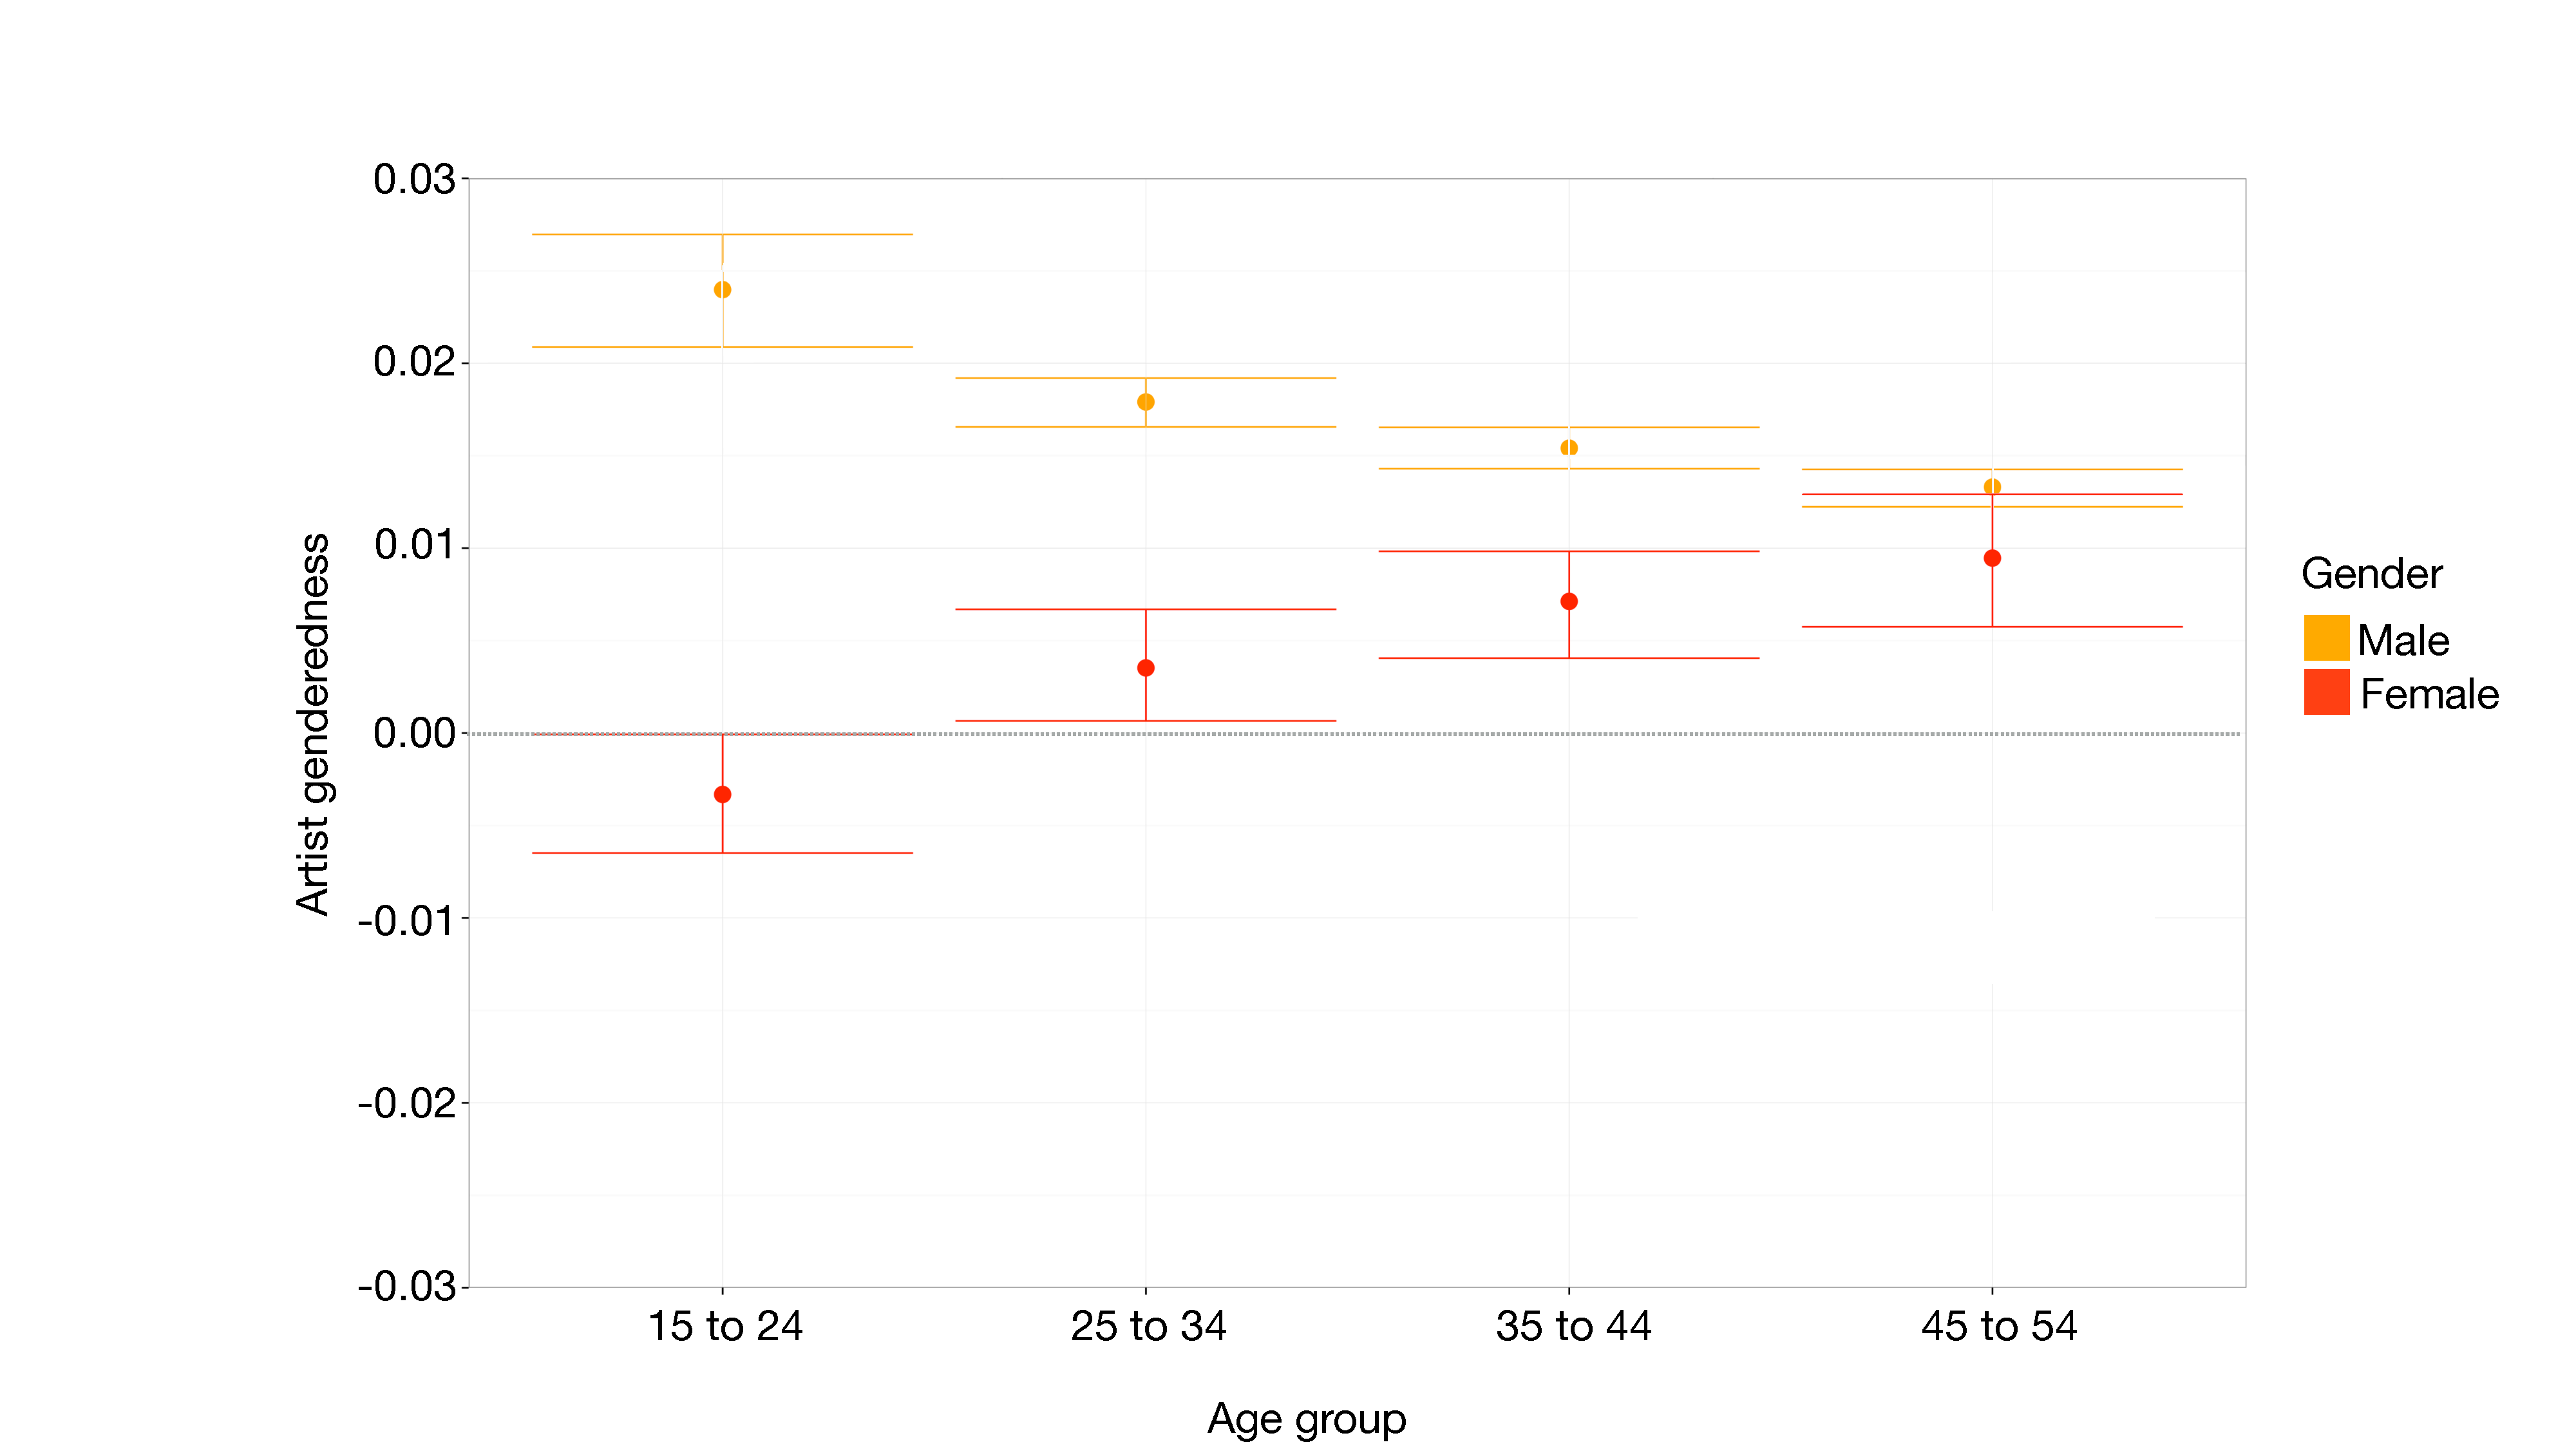
\includegraphics[width=0.9\textwidth]{artist_genderedness_by_age_groups_cropped.pdf}
\caption[Artist genderedness by age group and self-declared gender for balanced groups of listeners]{Artist genderedness by age group and self-declared gender for balanced groups of listeners (N = 200) of the MLHD. The dots indicate the mean and error bars show 95 percent confidence interval bars.}
\label{fig:artist_genderedness_by_age_groups_cropped}
\end{figure}




All in all, the user-centric listening features we designed seem to carry some relevant information about how listeners part of the MLHD listen to music. 
Since exploratoryness and mainstreamness showed the greatest differences across the different age groups we focused our efforts in using these two profiling characteristics.

In the next section we will describe how we compared the performance of music artists recommendation models by using several combinations of the listeners' demographic, profiling, and contextual features.

% % \subsection{Recommending music according to profiles of listeners}

% \subsection{Music recommendation with side features data}
% We now proceed to perform a mid-size experiment on prediction of ratings using the factorization machines approach presented by \textcite{rendle11fast}. 
% We randomly sampled our dataset and obtained 936554 observations for 1042 users on 132903 different artists. Rating values are assigned from the listeners' listening history, converting the per-artist listening frequencies (implicit rating feedback) into a 5-level likert scale of explicit rating feedback.
% The experiment consisted on finding a set of low-ranking matrixes that were able to regenerate the values for all ratings that the set of users have given to some of the artists in the dataset. Finding these lower-rank matrixes will also allow to predict the rating of users on artists they have not listened yet. 

% We split the dataset into training (.8) and testing (.2) subsets. Also, additional self-declared user-side demographics features such as age group, country, gender, and also profiling data extracted from the listening patterns themselves, such as \emph{artist mainstreamness} and \emph{artist exploratoryness}, were fed into the factorization machines model as side data features. 
% We expected that certain combinations of side-data features might have an impact in the computed RMSE error. Using the self-declared country, for example, might have an impact in the accuracy of the system.
% Also, for calculating the best set of parameters, we iterated on the number of latent factors (2, 20, 200), and $\lambda$ regularization factor (0.1, 0.01, 0.001, \num{1e-4}, \num{1e-5}, \num{1e-6}, \num{1e-7})

% \begin{figure}[ht]
% \vspace{1em}
% \centering
% 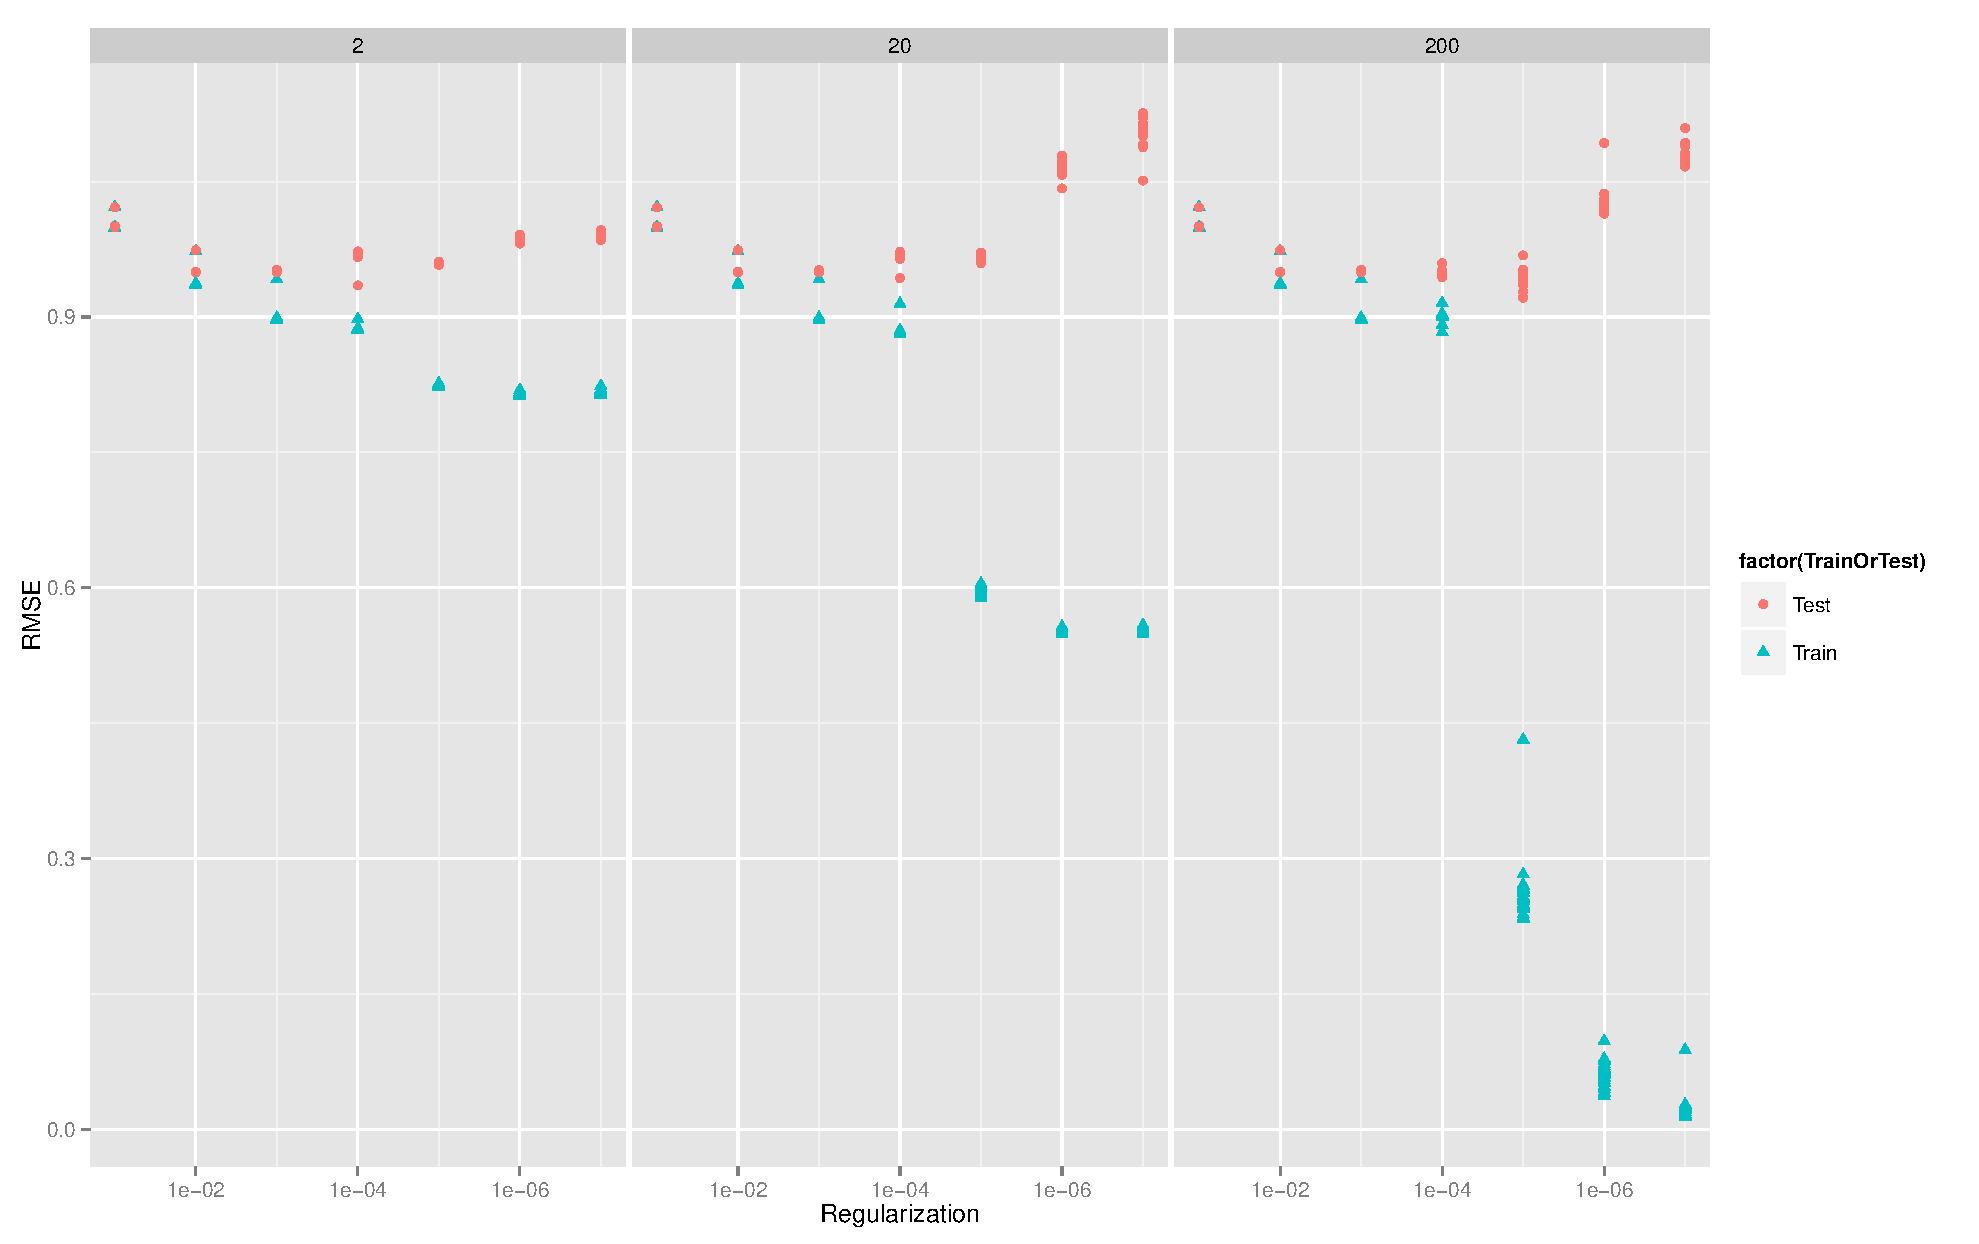
\includegraphics[width = 1.0\textwidth]{Train-test-RMSE-factors-regularization-side-data.pdf}
% \caption{RMSE values for training and testing sets, tested with three different number of latent factors (2, 20, 200), seven different $\lambda$ regularization values, and a set of 32 combinations of side-data features}
% \label{fig:Train-test-RMSE-factors-regularization-side-data}
% \end{figure}


% Fig.\ref{fig:Train-test-RMSE-factors-regularization-side-data} shows the computed RMSE values for the training and testing sets.
% It can be seen that the error obtained for both sets was similar for higher values of the $\lambda$ regularization value on each trial of the experiment with the three different number of factors.
% On the contrary, the computed error for both sets differed greatly for $\lambda$ values equal or smaller than \num{1e-5}. 
% Resulting error values in the testing dataset seemed not to be impacted by the number of latent factors used for training the system. In the testing set, however, the number of latent factors seemed to have an impact, particularly with smaller regularization values. 
% This behaviour indicates that, at least in this experiment, using smaller regularization values and larger number of latent factors led to overfitting the training data, obtaining smaller and desirable RMSE values, but making the learned model not generalizable to the testing dataset.



% Regarding side data features, it is interesting to note that since all 32 combinations seemed to get similar results in training and testing datasets, no combination of them exhibited a better performance. 
% This result is counter intuitive since it was expected that a combination of certain features, e.g., age group and country, might have led to smaller RMSE values. 
% Hence, are relevant for the recommendation of artists some side features such as the country, age, gender, or profiling features of the listeners? The trained model using these features led to similar results than the one that did not use them, and so according to the results just presented, they are not. In order to get deeper insights about user side features in the experiment, we proceeded to plot just the features that gave the best results in terms of RMSE in the testing dataset.

% \begin{figure}[ht]
% % \vspace{1em}
% \centering
% 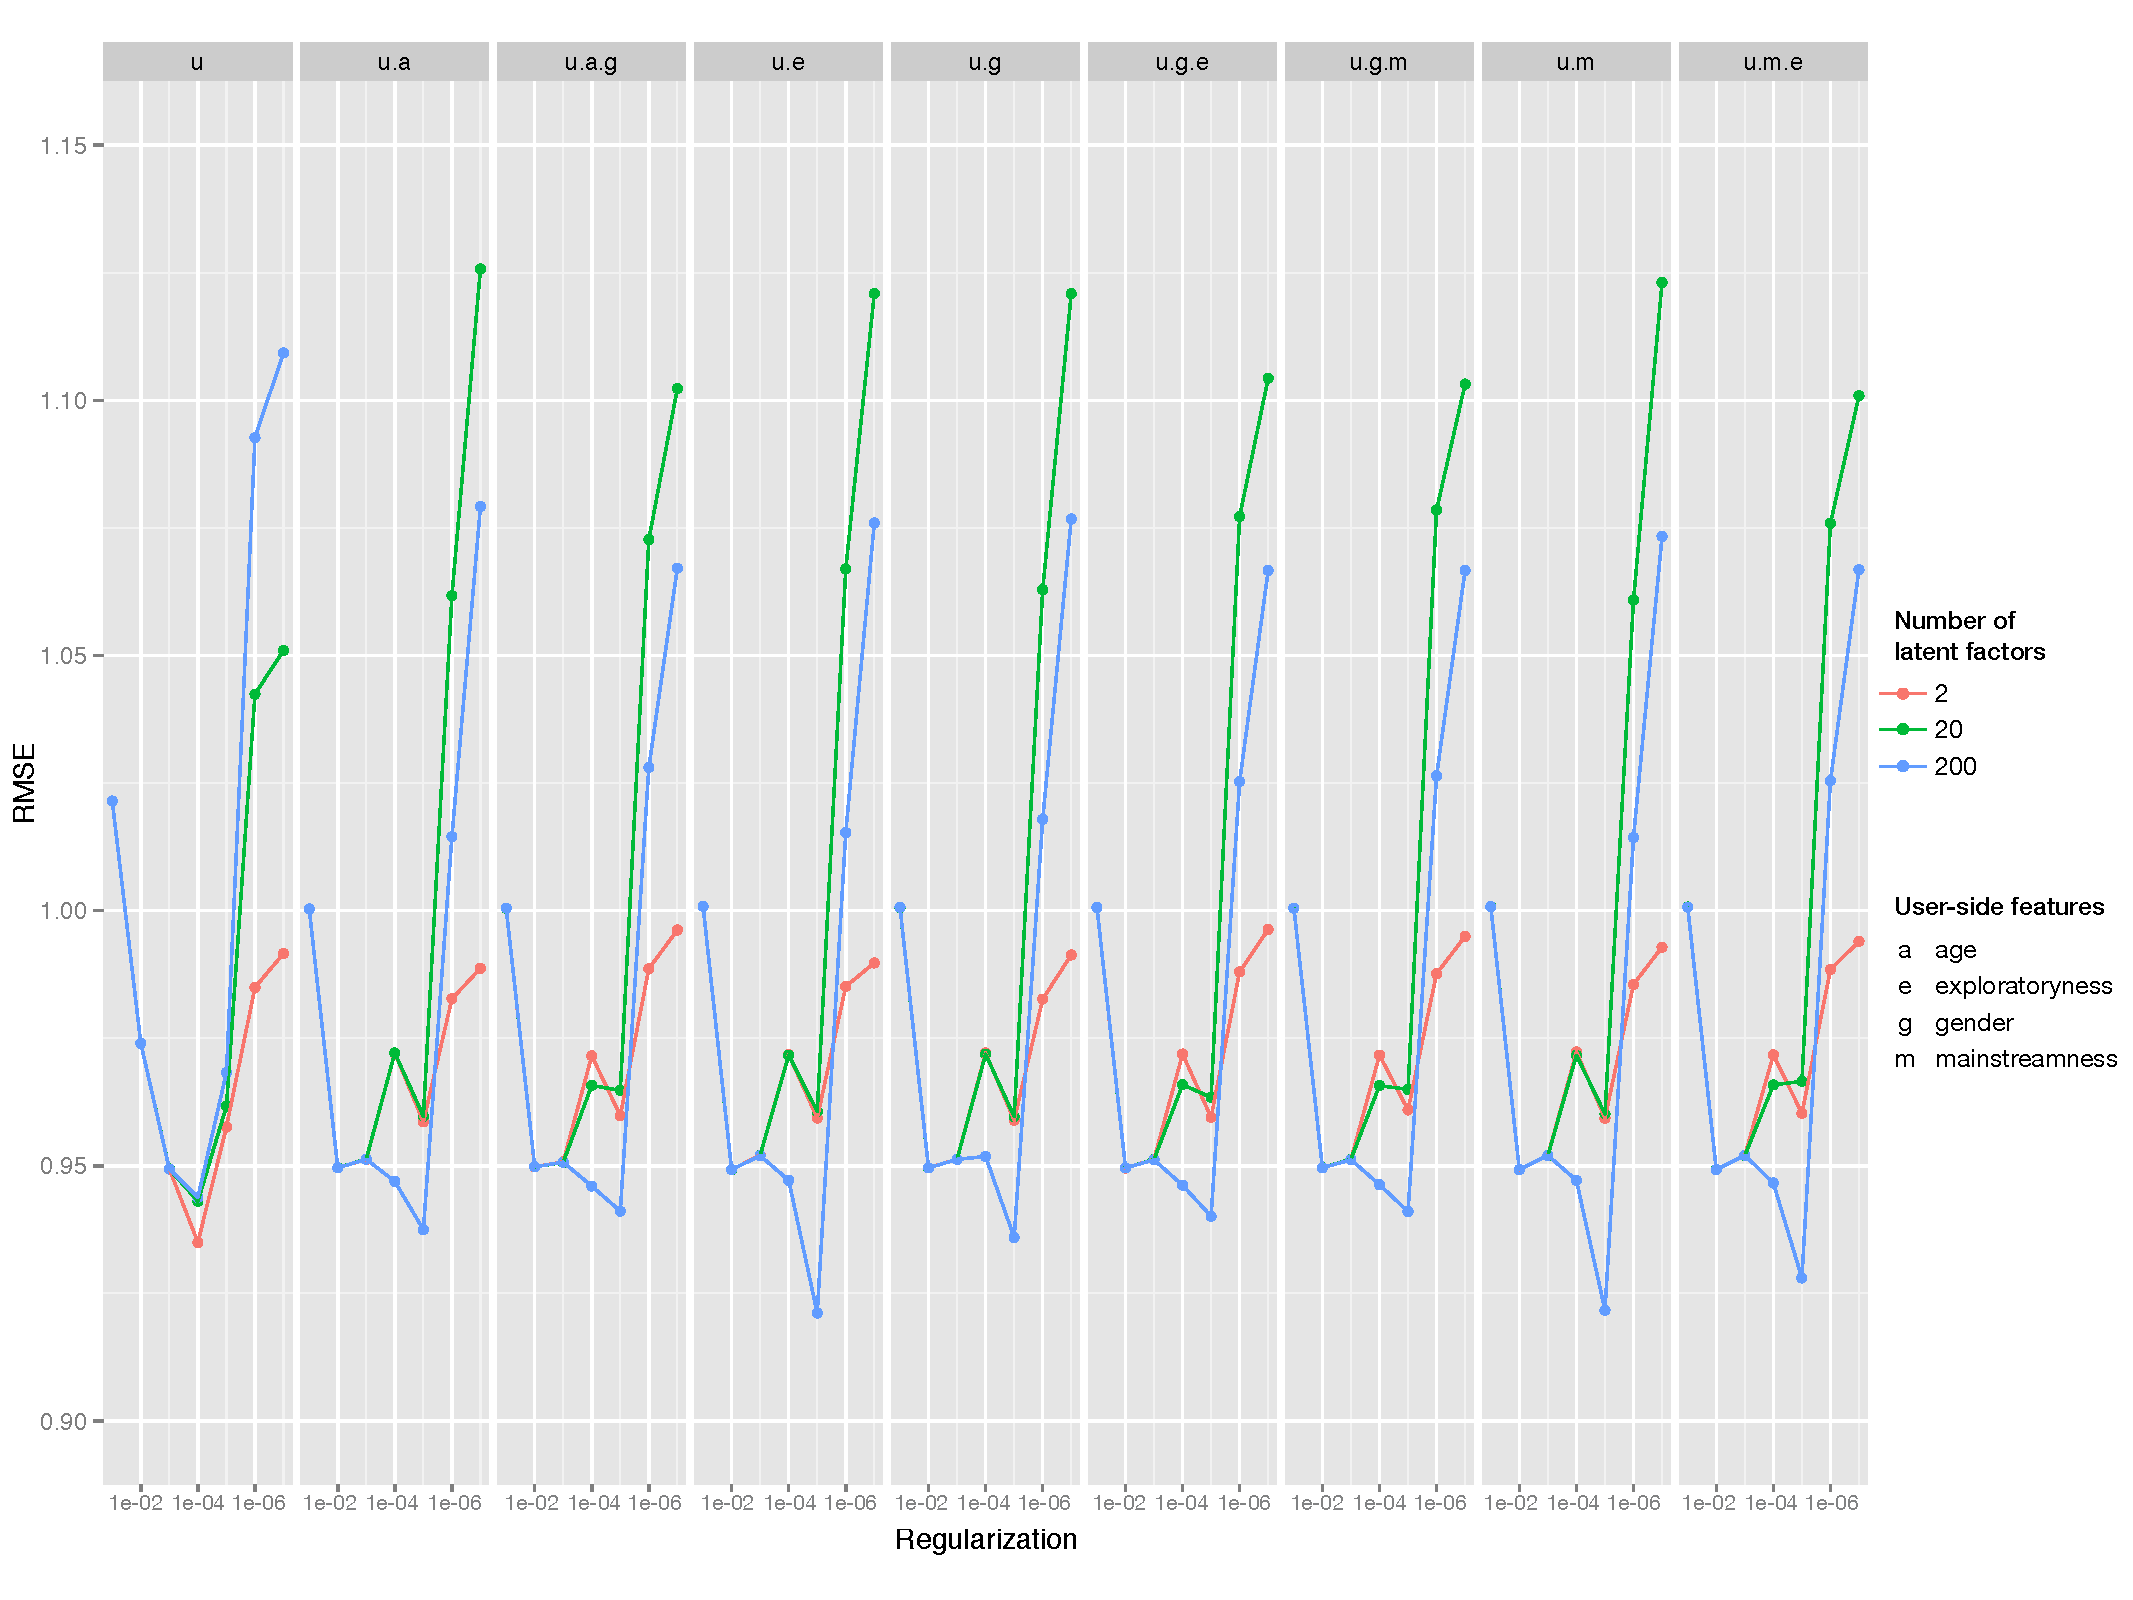
\includegraphics[width = 1.0\textwidth]{Train-test-RMSE-regularization-side-data_200_factors_3_K.pdf}
% \caption{Accuracy of the matrix factorization model. The plot shows root-mean-square error (lower is better) of each of selected nine different user-side features, evaluated with seven different regularization values, and three different number of latent factors. 
% Better accuracy was obtained by using increasing the dimensionality of the model to 200 latent factors, a regularization value of \num{1e05}, and using user's \emph{profiling} instead of \emph{demographics} features}
% \label{fig:Train-test-RMSE-regularization-side-data_200_factors}
% \end{figure}


% Fig.~\ref{fig:Train-test-RMSE-regularization-side-data_200_factors} shows a subset of nine feature combinations, for different regularization values, evaluated with 2, 20, and 200 latent factors. The first column \emph{u} corresponds to the results obtained with no user-side data for estimating the model, just plain matrix factorization with the known implicit feedback of users on artists. 
% As can be seen in the plot, the best RMSE value for the testing set (lower is better) was achieved in several trials by using the profiling features \emph{artist exploratoryness} and \emph{artist mainstreamness} alone, or in their combination, with no demographic features at all. Both features achieved almost the same error value of $.921$ with 200 latent factors and a $lambda$ regularization value of \num{1e-05}.

% These results show that there is not much relevant information in the demographics features to estimate a better prediction model. 
% This lack of impact of the demographics features is intriguing, since it was expected that age, country, or gender would have an effect in reducing the error of a model or, more clearly, in determining the preference of listeners for certain music items.
% On the contrary, there is some information encoded in the listeners' profiling features that help to estimate a better prediction model. 
% However, instead of thinking that demographics data is not relevant, it might be argued that collaborative filtering already has encoded, or expresses, some of the relations between users and their demographics, and so these features do not have a great impact in reducing the error. In other words, latent factors among users may have already some demographics data incorporated in it.

% % Some questions:
% % \begin{itemize}
% % \item The same results will be achieved if I run the test again?
% % \item In a bigger set?
% % \item How factorization machines predict ratings in a toy example? For example, by having people from the same, and different countries
% % \item What features from the item side could be used to improve recommendation? Artists' genre tags? Track' AB data?
% % \end{itemize}



% \subsubsection{Estimating preference model with weekly-aggregated listening data}


% Hypothesizing that people may have different listening preference patterns per music items on weekdays and weekends, we designed an experiment to determine if estimating a model using listening data from weekdays or weekends only, instead of full-week aggregated data, would return lower root-mean-square error values. 
% Hence, when computing RMSE of the estimated model with the testing dataset generated lower values with splits of the weekly listening data, instead of using the full week, that would imply that listeners have different listening preferences between weekdays and weekends because there would be less variance in their listening preferences in the two conditions.

% To test the hypothesis, we took a randomly sample 10 percent of listening histories from our full dataset, considering the artists they listened to. Three sub-datasets of listening histories were generated from this sample.
% The first dataset considered all listening data for all listeners, the second dataset only considered data from weekdays. Finally, the third dataset only considered weekend data. For the three datasets, and for each listener, a ranking of listening preference was generated, and a 5-level likert scale rating value was estimated from the frequency of listening per artist. Table~\ref{table:weekly_aggregated_listening_data} shows the total number of listeners and artists, and the total number of observations, i.e., the total number of implicit feedback-generated ratings.

% \begin{table}[ht]
% \vspace{1em}
% \centering
% 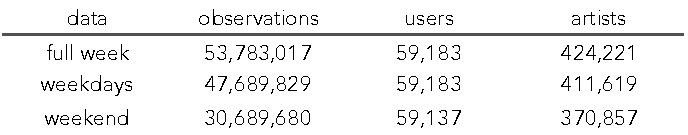
\includegraphics[width = 0.75\textwidth]{experiment_table.pdf}
% \caption{Number of total observations, users, and artists for the different splits of weekly aggregated listening data}
% \label{table:weekly_aggregated_listening_data}
% \end{table}

% From the table, it is possible to see that although the number of listeners is 10 percent of the total number of listeners in the original dataset, the coverage of artists is much larger---being close to 76 percent in the full week and 67 percent on the weekends---since the total number of artists in the dataset is 555K, as was shown in Table~\ref{table:dataset_summary}. This coverage implied that many artists were covered in the sub-datasets notwithstanding the small sample of listeners.


% Again, our procedure followed the approach by \textcite{hu08collaborative}, by factorizing the matrix of observations by two lower-dimensional matrices with a small number of latent factors, with the idea of minimizing the RMSE between the original preference matrix and the product of the two lower dimensional matrices. This procedure was repeated for the three datasets of the experiment. Several different $lambda$ regularization values as well as number of factors were tested in the model estimation in order to obtain the best set of variables for these datasets. 

% Fig.~\ref{fig:weekly_listening_experiment} shows the RMSE values for the training and testing datasets. 

% The chosen method for estimating the models was matrix factorization was Adagrad (Adaptive Stochastic Gradient Descent). The best RMSE values, overall, were found with a $lambda$ of \num{1e-6}.

% % \begin{figure}[h]
% % \centering
% % \includegraphics[width = 1.0\textwidth]{week_weekly_results.pdf}
% % \caption{Number of total observations, users, and items for the different splits of weekly aggregated listening data}
% % \label{fig:week_weekly_results}
% % \end{figure}




% \begin{figure}[ht]
% \vspace{1em}
% \centering
% 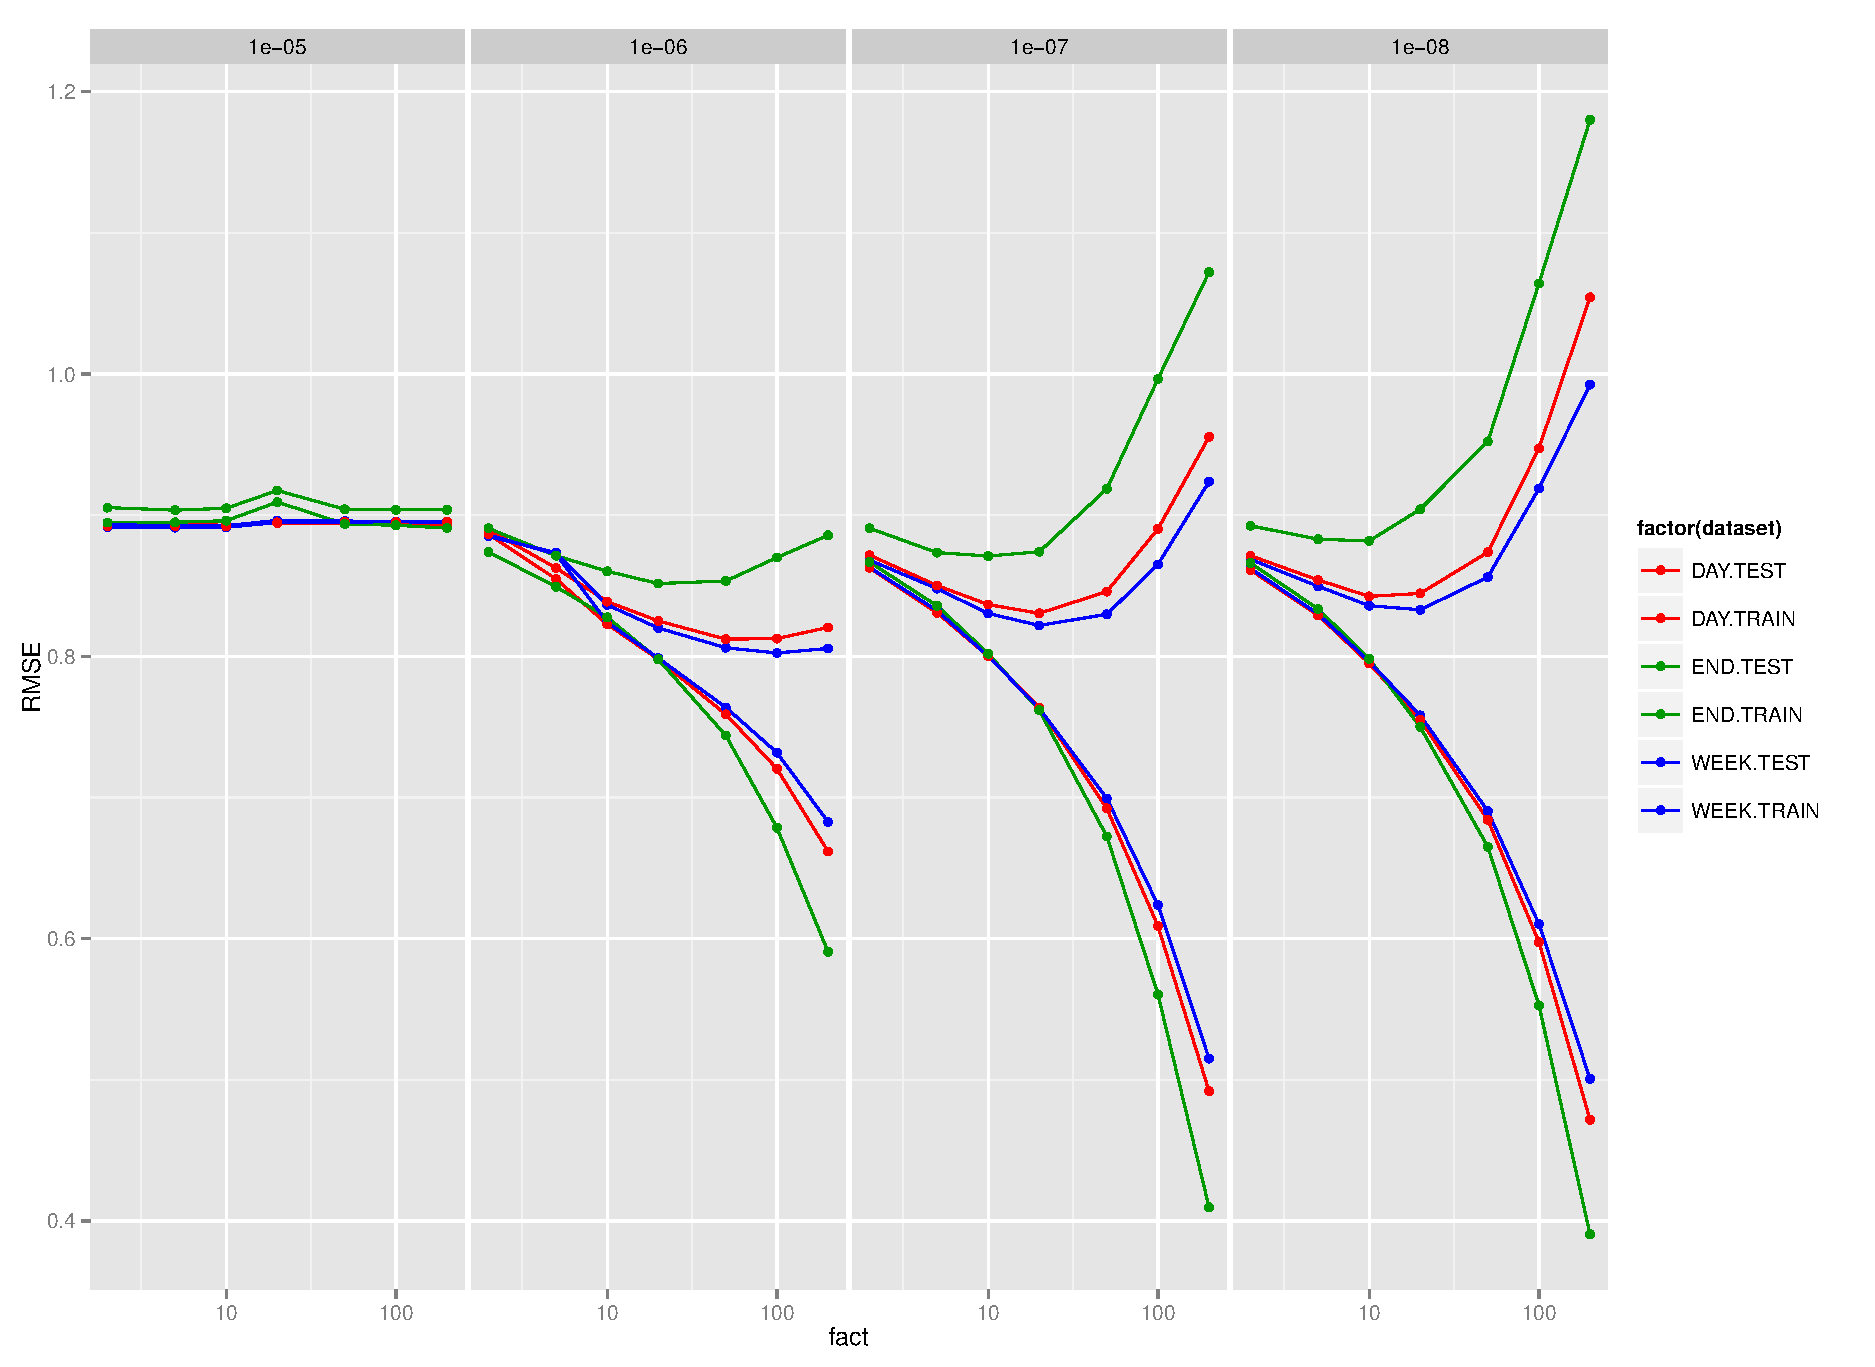
\includegraphics[width = 1.0\textwidth]{weekly_listening_experiment.pdf}
% \caption{Accuracy of the matrix factorization model. The plot shows root-mean-square error of training and testing datasets, for full week, weekdays, and weekend data, evaluated with seven different regularization values, and three different number of latent factors. 
% Better accuracy in the testing dataset was achieved by using the full week data, for all regularization values and number of factors.}
% \label{fig:weekly_listening_experiment}
% \end{figure}




% \singlespacing

% \subsubsection{Recommending music according to listener profiles}




















\section{Experiment implementation}\label{sec:6-experiment-implementation}
Our goal is to evaluate if demographics, behavioural profiles, and the use of observations from different contexts improve the accuracy of a recommendation model.
Our sources of data involve a matrix of user preferences on artists obtained from  implicit feedback derived from the users' music listening histories, 
% derived from implicit feedback, 
a set of three categorical demographic features for each user: \emph{age}, \emph{country}, and \emph{gender}, and a set of two continuous-valued features for describing listening behaviour: \emph{exploratoryness} and  \emph{mainstreamness}. Preference matrices were generated by considering \textit{full-week} music listening history data, as well as data coming from music logs submitted on \textit{weekdays} and \textit{weekends} only.

We followed a similar approach to \textcite{koren09matrix}, in which a matrix of implicit feedback values expressing user preference for items is modelled by finding two lower-dimensional matrices of rank $f$, $X_{n\times{f}}$ and $Y_{m\times{f}}$, whose product approximates the original preference matrix. The goal of this approach is to find the set of values in $X$ and $Y$ that minimise the RMSE error between the original and the reconstructed matrixes. 
However, this conventional approach of matrix factorisation for evaluating the accuracy of recommendation models using latent factors does not allow the researcher to incorporate additional features, such as the set of user-centric features we extracted and designed. 
% Hence, using extra features to characterize people's demographics or behaviour can not be represented with plain matrix factorization.

In order to incorporate latent factors as well as user-centric features into one single recommendation model, we used the Factorization Machines me\-thod for matrix factorisation and singular-value decomposition \autocite{rendle10factorization}. 
In this approach, interactions between the latent factors as well as the additional features are computed within a single framework, with a computational complexity that is linear to the number of extra features. 
Since the amount of interactions between side data features and latent factors can be large, a low computational complexity allows faster model learning speed.

% \subsection{Implicit into explicit feedback}\label{subsec:feedback}
We randomly sampled full music listening histories from 10 percent of all listeners in the MLHD in order to perform a series of experiments with different combinations of model parameters and user-side features in a timely fashion. We assumed that a random subset of listeners of this size would have similar statistical properties to the original dataset. 
We then aggregated the subset of listening histories by creating \small{\texttt{<user, artist, playcounts>}} \normalsize triples. 
We transformed the number of playcounts in each triple into a 1--5 Likert scale value by means of calculating the complementary cumulative distribution of artists per listener \autocite{celma10music}. Hence, artists in each distribution quintile were assigned with a preference value according to how much each user listened to them.

All in all, we ended up with a subset that had more than 60M ratings taken from the listening histories from 59K listeners. The total number of artists included in these listening histories was about 432K artists. We observed that the rating matrix was very sparse, exhibiting a density of observations of about 0.24 percent (density of observations is the inverse measure of sparsity).
In order to provide the reader with an idea of the size and characteristics of this subset, the Netflix Prize training dataset had 100M observations, taken from 480K users on 18K movies, with a density of 1.2 percent. 
The smaller density of observations in our subset implies that there were more rating interactions that had to be determined. 


% \subsection{Learning latent factors}\label{subsec:latent}
When performing matrix factorisation with a set of explicit or implicit preferences, the item ratings expressed by users, or inferred from their actions on the items, are mapped to a latent factor space of dimensionality $f$, in such a way that their interactions are approximated as the inner product in this space \autocite{koren09matrix}.
As a result, columns in the two resultant low-dimensional matrices correspond to $f$ unknown latent factors that may describe some aspects of the expressed preferences in the original rating matrix. 
These factors are features that have to be determined by the analyst but, for the sake of giving a few domain-specific examples, they could be the perceived music genre of an artist, the perceived valence of the artist's music, and the overall musical complexity.
Values in the columns of the first matrix represent how much a listener is interested in those specific characteristics and values in the columns of the second matrix indicate how much each artist exhibits those particular features.

For the sake of visualising if a latent factor model using matrix factorisation may learn something from the rating data in our subset, we estimated the latent factor values learned from the implicit ratings in the subset. In order to facilitate the visual inspection by transferring those values to a two-dimensional plot, we computed matrix decomposition with only two latent factors. 
In Figure \ref{fig:latent_factors} we show the two-latent factor decomposition of the subset rating matrix. A few selected popular artists are placed in the plot according to their corresponding learnt factor values. 

\graphicspath{{./figs/ch7/}}
  \begin{figure}[!h]
  \centering
  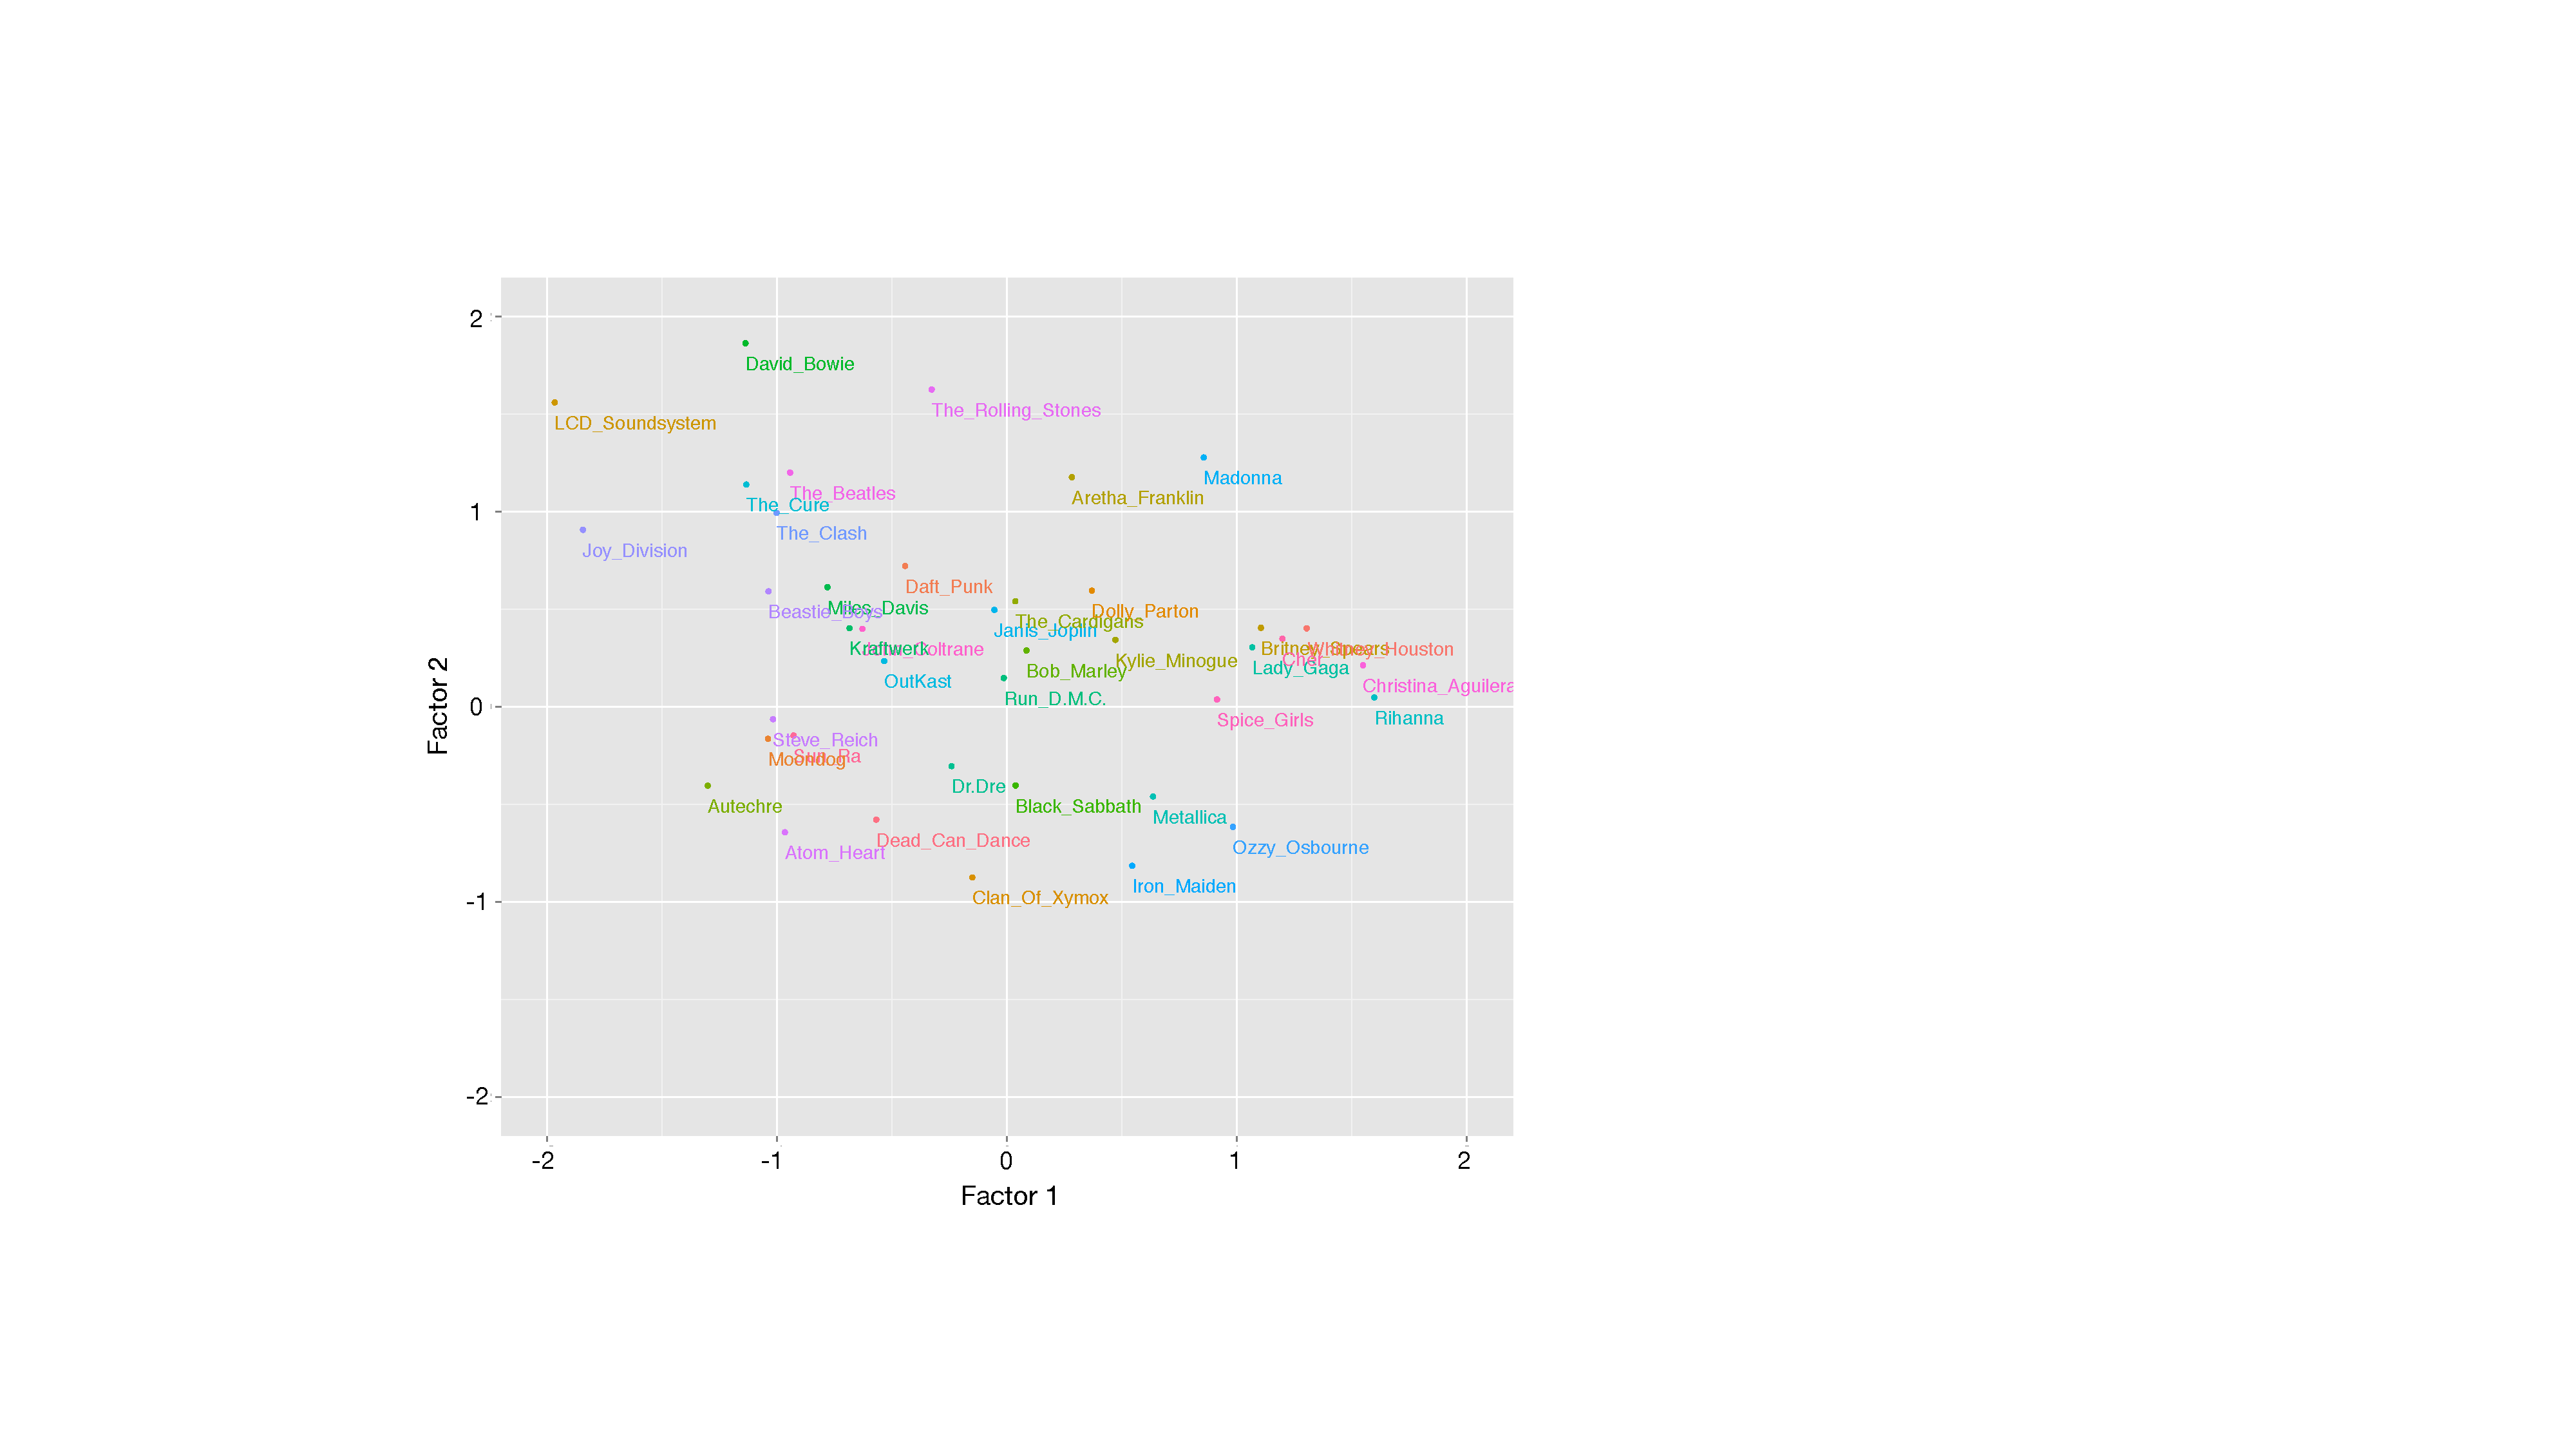
\includegraphics[width=0.9\textwidth]{latent_factors_1.pdf}
  \caption[Latent factor decomposition of the subset rating matrix]{Latent factor decomposition of the subset rating matrix. Only two factors were used for this representation. Selected artists are placed in the plot according to the learnt factors. Artists in the plot seem to be clustered by quadrant.}
%   The plot reveals that the artists are organised in clusters by quadrant.}
  \label{fig:latent_factors}
  \end{figure}



We can see in the figure that there seems to be some inner organisation within the quadrants. 
In the first quadrant (i.e., both factors are positive) all artists are female, with a few exceptions.
% , with the exception of Bob Marley that is very close to the origin, and Janis Joplin, which is very close to the Factor 1 axis. 
The second quadrant (i.e., the first factor is positive and the second is negative) groups all the artists than can be considered dark and heavy, such as Black Sabbath or Iron Maiden. 
Quadrant three clusters the artists that are more minimal or ``cerebral,'' such as Autechre, Atom Heart, or Dean Can Dance. 
Interestingly, this quadrant groups very close together the musicians Steve Reich, Moondog, and Sun Ra. These three artists are very different, but the three of them mostly compose instrumental music with experimental traces. It is also possible that listeners perceive something in common between these three artists that transcends genre.
Finally, quadrant four congregates artists that can be considered classics, such as David Bowie, The Beatles, and Miles Davis. 

Since these are latent factors learned from the model, it is up to the knowledge of the researcher to come up with a set of specific words or concepts to interpret the quadrants, or to assign names to the names of the axes of this representation. 
Also, we decomposed the matrix of preferences by using only two factors. A much better model (i.e., a set of lower-dimensional matrixes that, when multiplied, approximate the original matrix with lesser error) may be achieved by using a larger number of latent factors. For example, if using three latent factors, a third factor, orthogonal to the plane of factors one and two, may separate Kraftwerk and John Coltrane. They lie right next to each other in the two-dimensional representation but they may be far away if more dimensions are factored in.



In order to learn the best set of parameters of the recommendation model, we performed a grid search on the $\lambda$ regularization parameter as well as the $f$ number of latent factors without user-side data, just using  plain matrix factorisation for the matrix of  preferences of users on artists.
Finding a good $\lambda$ value helps to avoid overfitting the observed data by penalizing the magnitudes of the learned parameters. Finding the best $f$ number of factors helps to obtain a better recommendation accuracy while also providing a set of to-be-interpreted latent factors. 

We followed the dimensionality numbers of latent factors tested by \textcite{koren09matrix,dror11yahooa}, and we used the Graphlab Create framework\footnote{The Graphlab-Create machine learning library for Python is available at \url{https://pypi.python.org/pypi/GraphLab-Create}} to perform a grid search of $f$ factors in the range [50, 200], and $\lambda$ regularization values in the range $[\num{1e-5},\num{1e-8}]$.  
% We used the Graphlab Create framework\footnote{\url{https://pypi.python.org/pypi/GraphLab-Create}} to search over the number of latent factors in the range [50, 200] (following the dimensionality latent factor numbers proposed by~\textcite{koren09matrix,dror11yahooa}), and regularization values in the range $[\num{1e-5},\num{1e-8}]$. 
We used the Adaptive Stochastic Gradient Descent optimization algorithm \autocite{duchi11adaptive} and set the maximum number of iterations at 50. This number of iterations was chosen because there was no substantial improvement in the model beyond this number.
The best combination of parameters was achieved for $\lambda$=$\num{1e-7}$ and $f$=50 latent factors. 
% 6.22\text{\sc{e}-}21
% same thing: $1\e{-5}$.



%   \begin{figure*}[t]
%   \centering
%   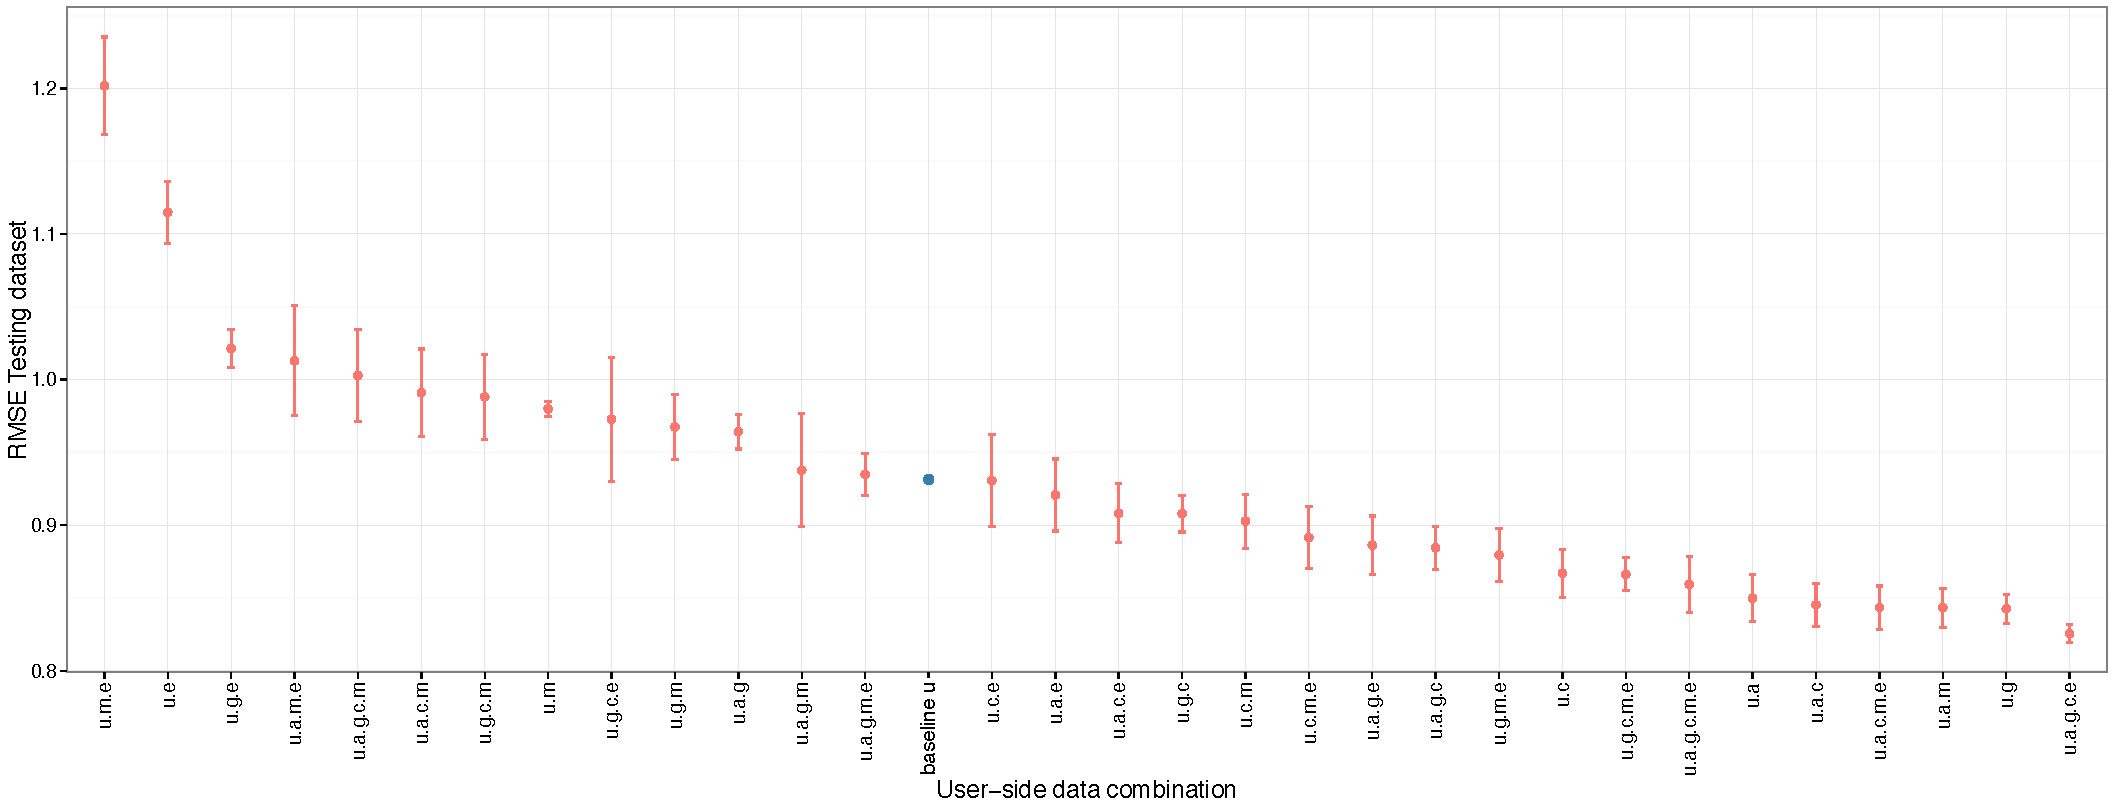
\includegraphics[width=1.0\linewidth,keepaspectratio]{figs/ch8/32_features_1e-06_100_factors_ci__n_5_bootstrap_100_publication_cropped-2_to_crop_cropped.pdf}
%   \caption{Root mean square error means and 95 percent CI bars for learned models evaluated in the testing dataset, with 32 combinations of the user-side features, ranked in decreasing order. Feature combinations are labelled according to the first letter of the word they represent. Baseline for comparison is combination \emph{u}: user's preferences only, without any user-side features. }
%   \label{fig:4_feature_comparison_results}
%   \end{figure*}


% Root mean square error

\subsection{Demographic and profiling features}
After the subset was created, we split it into two disjoint sets: training (90 percent) and testing (10 percent) datasets. 
With the best set of hyper-parame\-ters of the model already estimated, we evaluated the recommendation accuracy in the testing dataset of models learned from the training data for all combinations of user-side demographic and profiling features. 
Since we had five user-side features (i.e., age, gender, country, exploratoryness, and mainstreamness) there were 32 (i.e., $2^5$) different combinations. 

Learning a model using an optimization algorithm can sometimes cause the results to converge into local minima instead of the global minimum,  and so we repeated the process of learning and testing the accuracy of the learned models  10 times for each user-side feature combination.  Using this procedure, we also wanted to compare and evaluate if results in model error were similar throughout several trials.
The experiment baseline was established as the approach in which plain matrix factorisation was used to estimate the recommendation accuracy of the learned models by just using the matrix of preferences of listeners on artists, without any user-side  feature combination. By using this approach, we will able to compare if the use of any feature combination resulted in a decrease in RMSE error, thus indicating an increase in the accuracy of the model.

Figure \ref{fig:4_feature_comparison_results} summarises the results of all trials for all feature combinations. It shows all combination means, ranked in decreasing order, with 95 percent CI error bars generated from a bootstrap sample of 100 replications of the original sample. 
Feature combinations are labelled according to the first letter of the word they represented. For example, user preference data with age, gender, and exploratoryness is labelled \emph{u.a.g.e}; user data with no user-side feature combinations is just labelled \emph{u}.


\begin{sidewaysfigure}
    \centering
  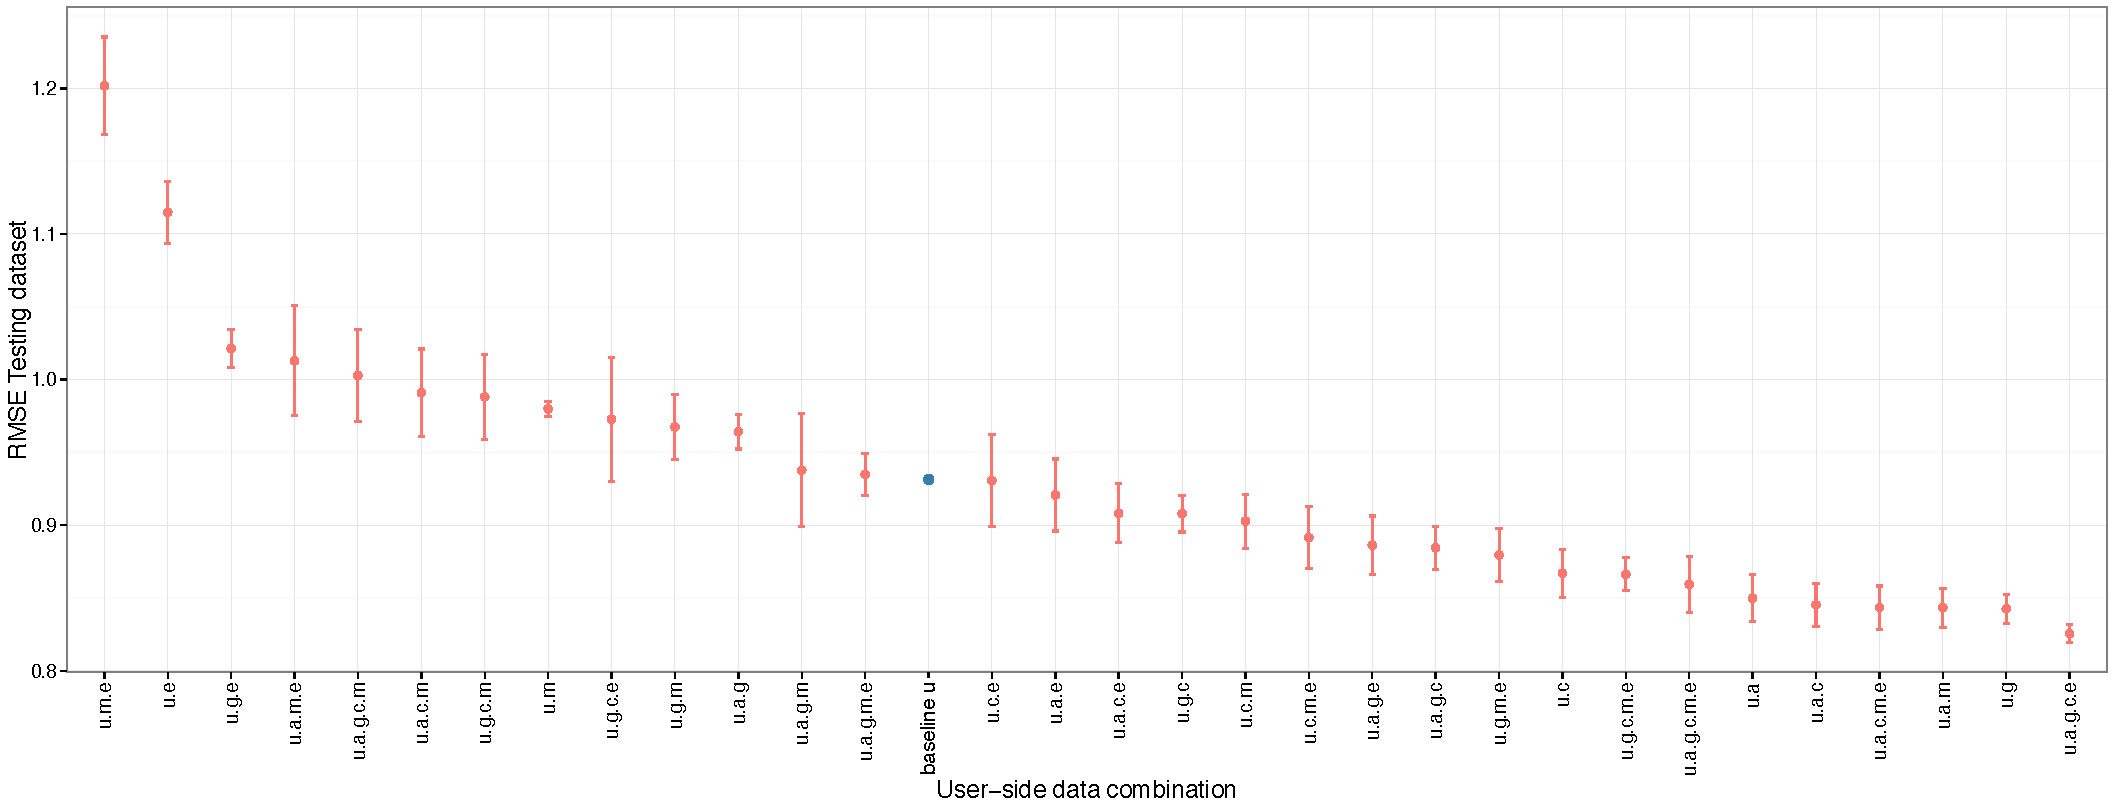
\includegraphics[width=1.0\linewidth]{figs/ch8/32_features_1e-06_100_factors_ci__n_5_bootstrap_100_publication_cropped-2_to_crop_cropped.pdf}
  \caption[Root mean square error means for learnt models with 32 combinations of user-centric features, ranked in decreasing order]{Root mean square error means and 95 percent CI bars for learnt models evaluated in the testing dataset, with 32 combinations of the user-centric features, ranked in decreasing order. Feature combinations are labelled according to the first letter of the word they represent. Baseline for comparison is combination \emph{u}: user's preferences only, without any user-side features. }
  \label{fig:4_feature_comparison_results}
\end{sidewaysfigure}





It can be seen that \emph{u}, the baseline without user-side features, achieved an average RMSE value of .931 and exhibited a small variability, indicating that models in this setup were stable across all  trials. All feature combinations to the right of the \emph{u} show a smaller RMSE error, thus providing evidence for an increase in the learned accuracies of those models. 
% usando regla de tres
% u.a: 100*(1-(.850/.931)) = 8.7%
% u.c: 100*(1-(.867/.931)) = 6.9%
% u.g: 100*(1-(.843/.931)) = 8.4%
% u.a.c.g.e.m: 100*(1-(.859/.931)) = 7.7%
% u.a.c.g.e: 100*(1-(.823/.931)) = 11.6%

Several feature combinations achieved better accuracy than the baseline. In particular, those combinations using just one of the demographic features: country (\emph{u.c}), age (\emph{u.a}), or gender (\emph{u.g}) achieved improvements of about seven, eight, and 
nine percent, respectively. Also, the combinations of only demographic features (\emph{u.a.g.c}) and all demographic and profiling features (\emph{u.a.g.c.e.m}) improved the baseline model by almost eight percent. However, the feature combination that achieved the best result was all demographic features together, plus the listener profiling feature of exploratoryness (\emph{u.a.g.c.e}), exhibiting an improvement of about 12 percent above the baseline. The small variability in the model error of this combination throughout all trials suggests that models based on this user-side feature combination were quite stable.
On the other hand, the combination of profiling features (\emph{u.m.e)} achieved the worst performance, with a 29 percent increase in error and a large variability in the estimated model error throughout trials. The variability in the results with these features suggests that the data topology using only profiling features is complex, probably making the iterative process of optimization converge into non-optimal local minima in the data. 
% In other words, by adding only these features make no small changes in the weight (factor) values would reduce the average error.%~\textcite{lecun15deep}
% 100-(100*1.201/0.931)

% It is also worth to mention that models with a much better recommendation accuracy were learned in some of the trial.  However, the topology of the data, in particular those combinations with more features, made the models to converge at  non-optimal points, and so their creation was not always stable. By looking at the variability of the RMSE results on each feature combination we can see that the more stable models were created with no user user side data (\emph{u}), followed by using people's age group (\emph{u.a}).


% no combination with more than three features achieved a statistically significant better result. 




% improvement =100*(1-(feat_comb_RMSE/baseline_RMSE))
% 100*(1-(.850/.931))

% Interestingly, none of the winners approaches of the Netflix prize used any external source of information, such is linking the movies with other databases of genre, for example (though the dataset provided movie names and release year)

\subsection{Listening preferences in the contexts of entire week, weekdays only, and weekends only}
% We also wanted to determine if context of listening affects the preferences of people on artists. 
We hypothesised that if people listen to music differently during the weekdays than on weekends, we could create more accurate models by using data from only the weekdays or weekends, respectively.
To test this hypothesis, we performed the same experimental approach that we carried out with the full-week dataset. 
However, this time we created two additional preference matrices of listeners for artists.
The first additional matrix was made by using only music logs submitted during weekdays, and the second matrix was made by  using only weekend music logs. 
Therefore, two extra sub-datasets were created using the original full-week dataset: \emph{weekday} and \emph{weekend} datasets. We then followed the same procedure described  before: we split the data into training and testing datasets, we learned models from the training dataset across all 32 combinations of user-side  features, and evaluated the accuracy of those models in the testing dataset. 
The number of observations, listeners, and density for each one the datasets are shown in Table \ref{tab:3_datasets}.


% \vspace{1em}
\begin{table}[h]
 \caption{Number of observations, listeners, artists, and density for each context-based preference matrix.} \label{tab:3_datasets}
 \begin{center}
 \small
\begin{tabular}{ccccc}
  \hline
  Dataset & Observations & Listeners  & Artists  & Density \\
  \hline
  Full-week  & 61M & 59K & 432K & 0.237\%\\
  Weekdays & 54M & 59K & 419K & 0.216\% \\
  Weekends & 35M & 59K & 379K & 0.154\%\\
  \hline
 \end{tabular}
\end{center}

\end{table}

As expected, the number of observations decreased in the datasets with partial data in relation to the full-week dataset. The number of listeners remained constant, which implies that most listeners in  the dataset submitted music logs during weekdays as well as on weekends.  Interestingly, the total number of artists for which there were submitted music logs on weekdays and weekends decreased between three and 12 percent in relation to the full-week data, which implies that many artists in the dataset were only listened during one of the two weekly periods. 
However, since there are many artists that have been listened to just a few times (i.e., they lie in the long tail), this behaviour is expected.
% The three preference matrixes show a very low density, indicating that preference data is sparse, meaning that listeners only have had experienced just a small portion of all available artists in the dataset.
% weekend artists' percentage in comparison to fullweek = 100-(37900/432)
The model accuracies obtained using music log data from the three aforementioned contexts are summarised in Figure \ref{fig:5_context_comparison_result}. 

\begin{figure}[!h]
	\centering
	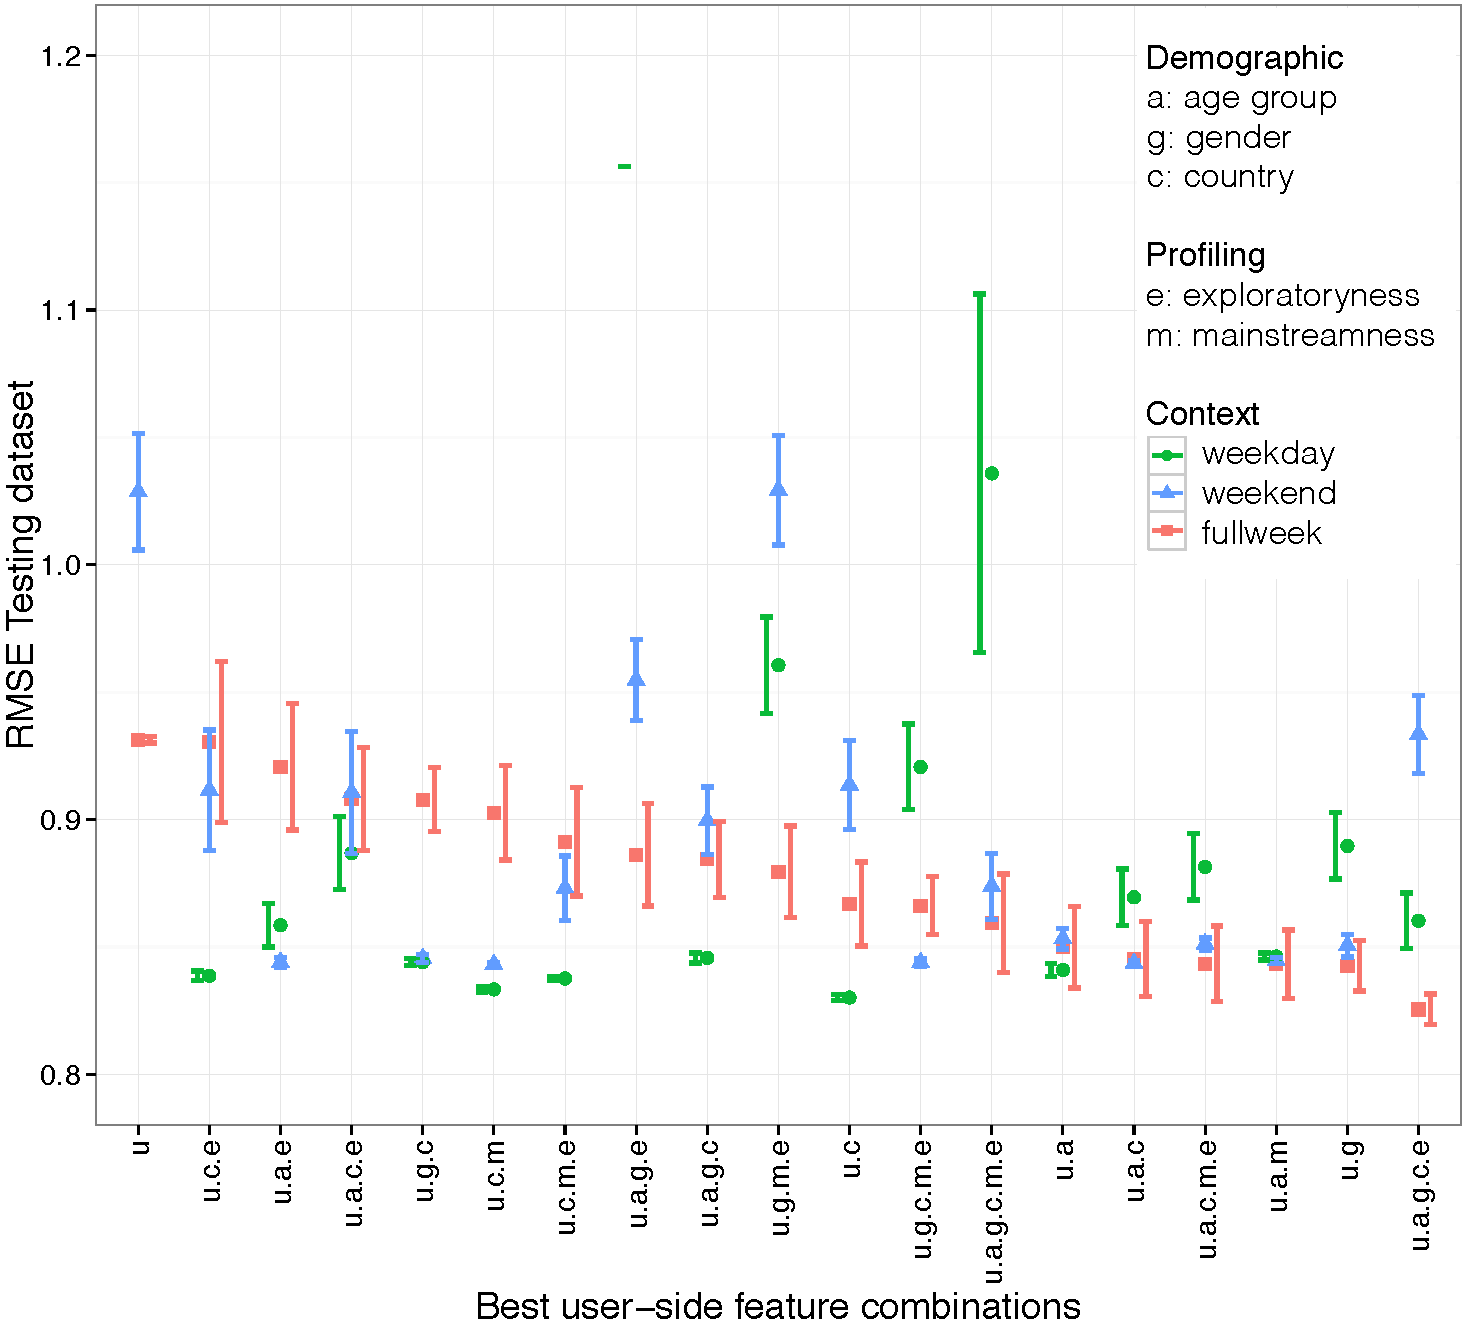
\includegraphics[width = 0.8\textwidth]{figs/ch8/best_features_dow_3_n_5_boostrap_100-1_legend_cropped.pdf}
 	\caption[Root mean square error means for learnt models with weekday, weekend, and full-week data]{Root mean square error means and 95 percent CI bars for learnt models with weekday, weekend, and full-week data. Only those feature combinations with a better RMSE value than the baseline for full-week data are shown.}
 	\label{fig:5_context_comparison_result}
\end{figure}


% Only those feature combinations with a better RMSE value than the baseline for full-week data are shown. 
Many of the models made with weekly split listening data achieved better performance than those using full-week data.  For example, models learned with weekday as well as weekend data using feature combinations \emph{u.a.e}, \emph{u.g.c}, and \emph{u.c.m} achieved improvements in accuracy of about seven percent in comparison to the model created with full-week data. They also showed smaller variability meaning more stability in model estimation.
However, while the best RMSE value was obtained using the user-side feature combination \emph{u.a.g.c.e} with full-week data, the same feature combination achieved worse performances by using listening data from weekdays and weekends only. 





% u.a.e 0.9207128 wf 
% u.a.e 0.8439785 we 100-(0.844*100/0.921) = 8.4 percent
% u.a.e 0.8585193 wd 100-(0.859*100/0.921) = 6.7 percent

% u.c.m 0.9026590 wf 
% u.c.m 0.8431579 we 100-(0.843*100/0.903) = 6.6
% u.c.m 0.8333907 wd 100-(0.833*100/0.903) = 7.8

% u.a.g.c.e 0.8255177 wf
% u.a.g.c.e 0.9334277 we 100-(0.933*100/0.826) = -13 percent
% u.a.g.c.e 0.8603450 wd 100-(0.860*100/0.826) = -4 percent


% \section{Conclusions and future work}

We have evaluated the impact of listeners' demographic and profiling features as well as basic forms of listening context, namely weekday and weekend versus full-week listening, on recommendation accuracy.
We described our requirements for a dataset of music listening histories, explaining why none of the  available datasets met our needs and how we ended up collecting our own data. 
We then formalised a set of listening behaviour profiling features that account for how much people explore music (exploratoryness), and how much they tend to listen to the same music as everyone else (mainstreamness). We also explained how we split our dataset of listening histories into weekdays  and weekend listening histories to evaluate if having data from different sets of listening histories improved the accuracy of recommendation.
Finally, we described how we set experiments that evaluated all combinations of user-side data features across different listening contexts. We found that the feature combination that achieved the smallest error was all demographic features together plus  listener's exploratoryness, obtaining 12 percent improvement over the baseline of not using any user-side feature data. 
Although for some feature combinations the use of split listening data improved the recommendation, the best combination of features did benefit from having full-week data. 
The lack of improvement in recommendation accuracy by means of using split-week data does not support previous research that found significant difference in listening behaviour between workdays and weekends using Twitter-based music listening data \autocite{schedl13leveraging}. The authors, however, used an approach based on the correlation of Last.fm tags assigned to artists per weekdays and weekends.
% We achieved these results using all available music items in the datasets, not just the most popular ones, as in previous experiments.

The results, in particular the many low RMSE values for several feature combinations using split listening data, seem to indicate that these error values are close to the limit in the minimum achievable error. This characteristic has already been described in the literature as a ``magic barrier'' in recommender systems design \autocite{herlocker04evaluating, bellogin14magic}, referring to the upper bound in rating prediction accuracy due to inconsistencies in user's ratings. However, since we are mapping the number of submitted music listening logs into ratings, we do not see how these inconsistencies can explain this barrier. In other words, our approach of using implicit, instead of explicit, feedback does not leave much space for user inconsistency.
Along these lines, it would be interesting to perform a narrower grid search in order to investigate if we are actually hitting a wall in accuracy, or if there is a better set of model parameters that allows us to create more stable models and  better performances throughout many trials.
% We have found that the best user side data feature combination improves the recommendation accuracy in 12 percent in average, in comparison to not using any side features. 
% By using the factorization machines modelling approach, we can also make recommendations not based on previous preferences of users on music items, but on same of their profiling or demographic features.
Finally, although these results show an improvement in the accuracy of a recommendation model based on listeners' past listening histories, a user-centred study may be carried out in order to measure people's actual satisfaction with the learned model.

In this chapter we described a set of features we developed to describe aspects of people's music listening behaviour. We also correlated these characteristics with listeners' self-declared demographic features and found some patterns that support and also that contradict previous findings using user-driven studies.
We finalised this chapter by evaluating the performance improvement of a music recommendation model by using the set of user-centric features.


% We now proceed to perform a mid-size experiment on prediction of ratings using the factorization machines approach presented by \textcite{rendle11fast}. 
% We randomly sampled our dataset and obtained 936554 observations for 1042 users on 132903 different artists. Rating values are assigned from the listeners' listening history, converting the per-artist listening frequencies (implicit rating feedback) into a 5-level likert scale of explicit rating feedback.
% The experiment consisted on finding a set of low-ranking matrixes that were able to regenerate the values for all ratings that the set of users have given to some of the artists in the dataset. Finding these lower-rank matrixes will also allow to predict the rating of users on artists they have not listened yet. 

% We split the dataset into training (.8) and testing (.2) subsets. Also, additional self-declared user-side demographics features such as age group, country, gender, and also profiling data extracted from the listening patterns themselves, such as \emph{artist mainstreamness} and \emph{artist exploratoryness}, were fed into the factorization machines model as side data features. 
% We expected that certain combinations of side-data features might have an impact in the computed RMSE error. Using the self-declared country, for example, might have an impact in the accuracy of the system.
% Also, for calculating the best set of parameters, we iterated on the number of latent factors (2, 20, 200), and $\lambda$ regularization factor (0.1, 0.01, 0.001, \num{1e-4}, \num{1e-5}, \num{1e-6}, \num{1e-7})

% \begin{figure}[ht]
% \vspace{1em}
% \centering
% 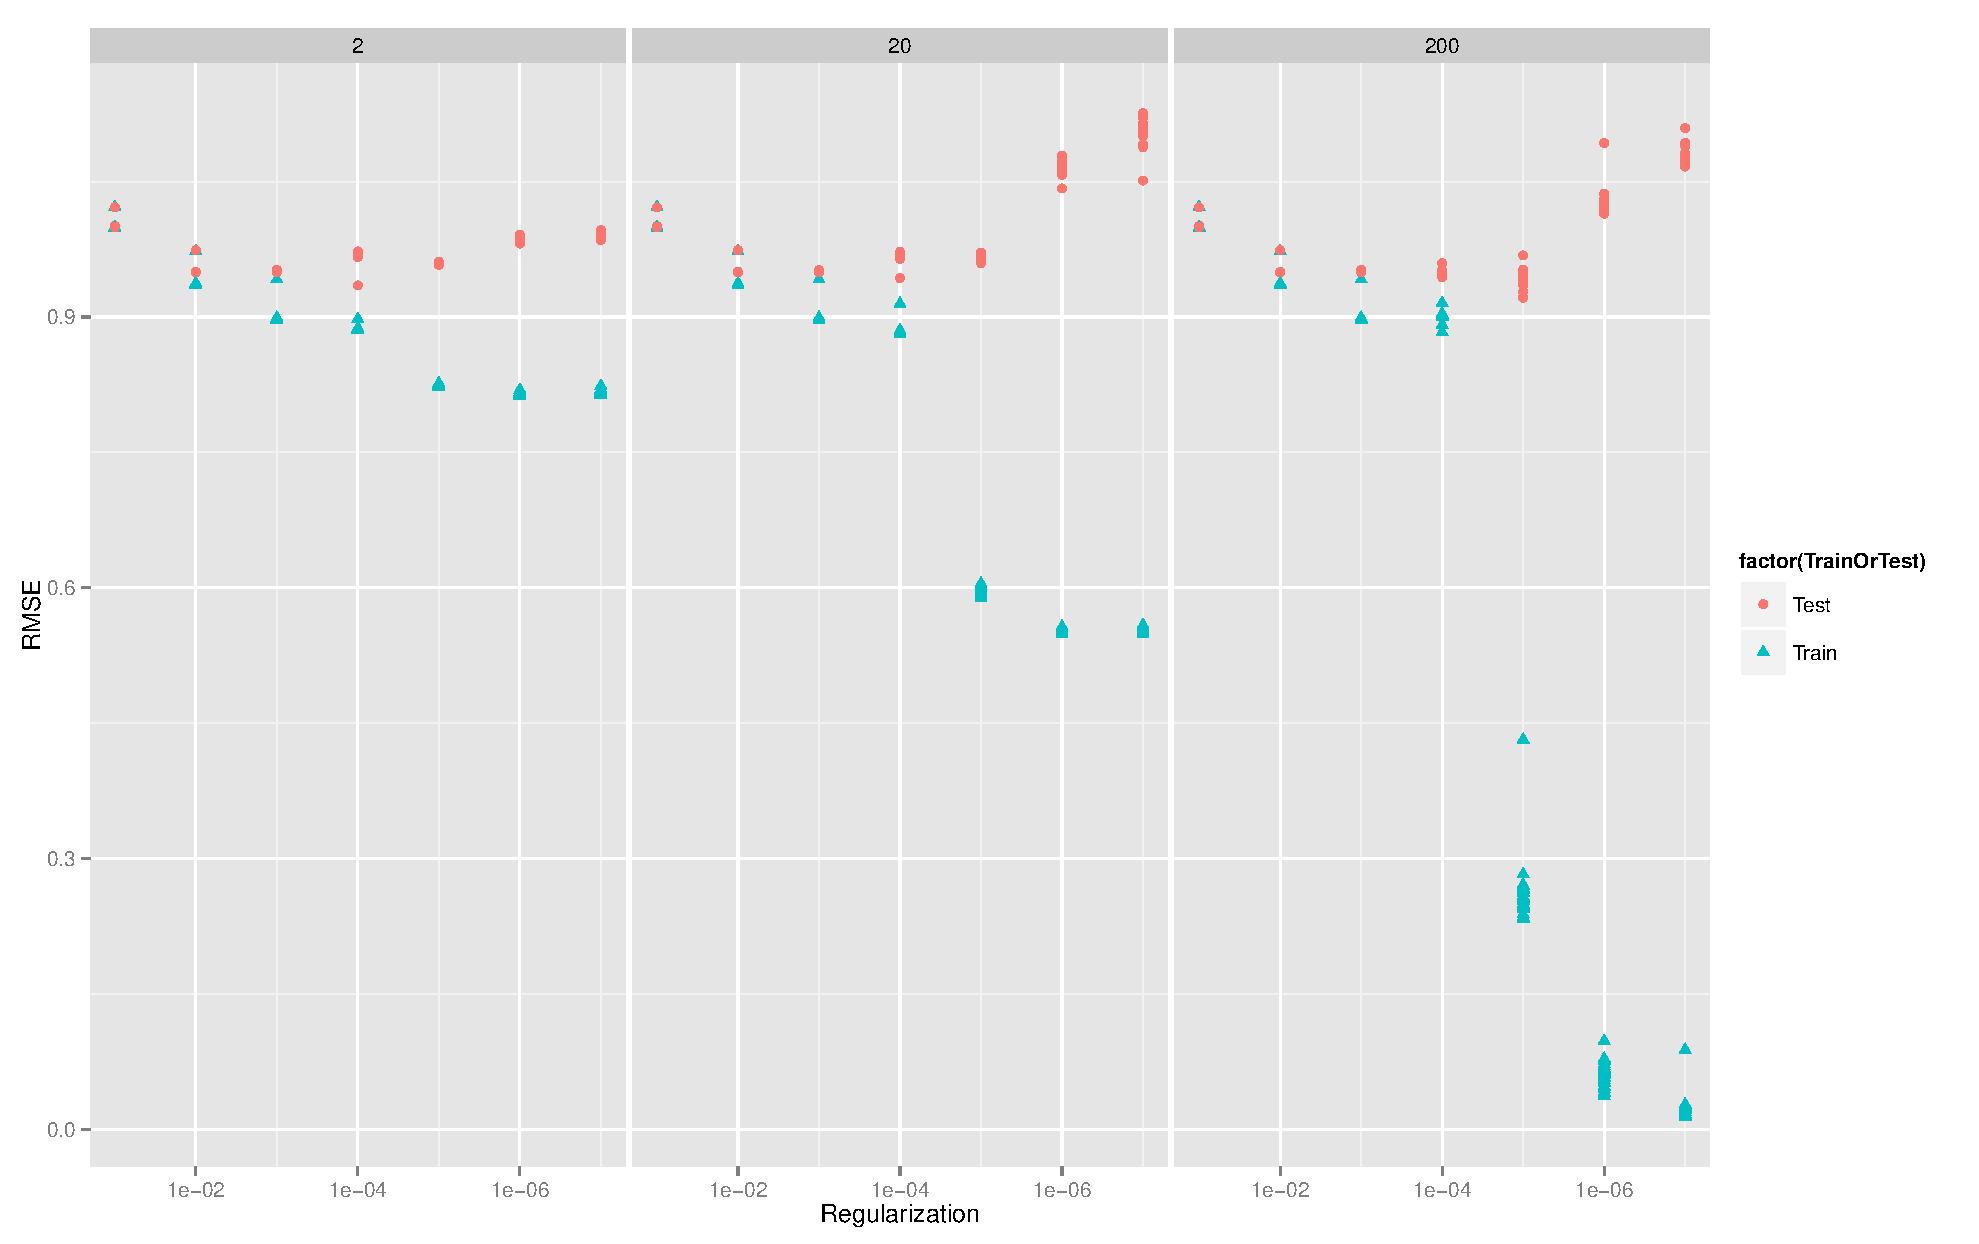
\includegraphics[width = 1.0\textwidth]{Train-test-RMSE-factors-regularization-side-data.pdf}
% \caption{RMSE values for training and testing sets, tested with three different number of latent factors (2, 20, 200), seven different $\lambda$ regularization values, and a set of 32 combinations of side-data features}
% \label{fig:Train-test-RMSE-factors-regularization-side-data}
% \end{figure}


% Fig.\ref{fig:Train-test-RMSE-factors-regularization-side-data} shows the computed RMSE values for the training and testing sets.
% It can be seen that the error obtained for both sets was similar for higher values of the $\lambda$ regularization value on each trial of the experiment with the three different number of factors.
% On the contrary, the computed error for both sets differed greatly for $\lambda$ values equal or smaller than \num{1e-5}. 
% Resulting error values in the testing dataset seemed not to be impacted by the number of latent factors used for training the system. In the testing set, however, the number of latent factors seemed to have an impact, particularly with smaller regularization values. 
% This behaviour indicates that, at least in this experiment, using smaller regularization values and larger number of latent factors led to overfitting the training data, obtaining smaller and desirable RMSE values, but making the learned model not generalizable to the testing dataset.



% Regarding side data features, it is interesting to note that since all 32 combinations seemed to get similar results in training and testing datasets, no combination of them exhibited a better performance. 
% This result is counter intuitive since it was expected that a combination of certain features, e.g., age group and country, might have led to smaller RMSE values. 
% Hence, are relevant for the recommendation of artists some side features such as the country, age, gender, or profiling features of the listeners? The trained model using these features led to similar results than the one that did not use them, and so according to the results just presented, they are not. In order to get deeper insights about user side features in the experiment, we proceeded to plot just the features that gave the best results in terms of RMSE in the testing dataset.

% \begin{figure}[ht]
% % \vspace{1em}
% \centering
% 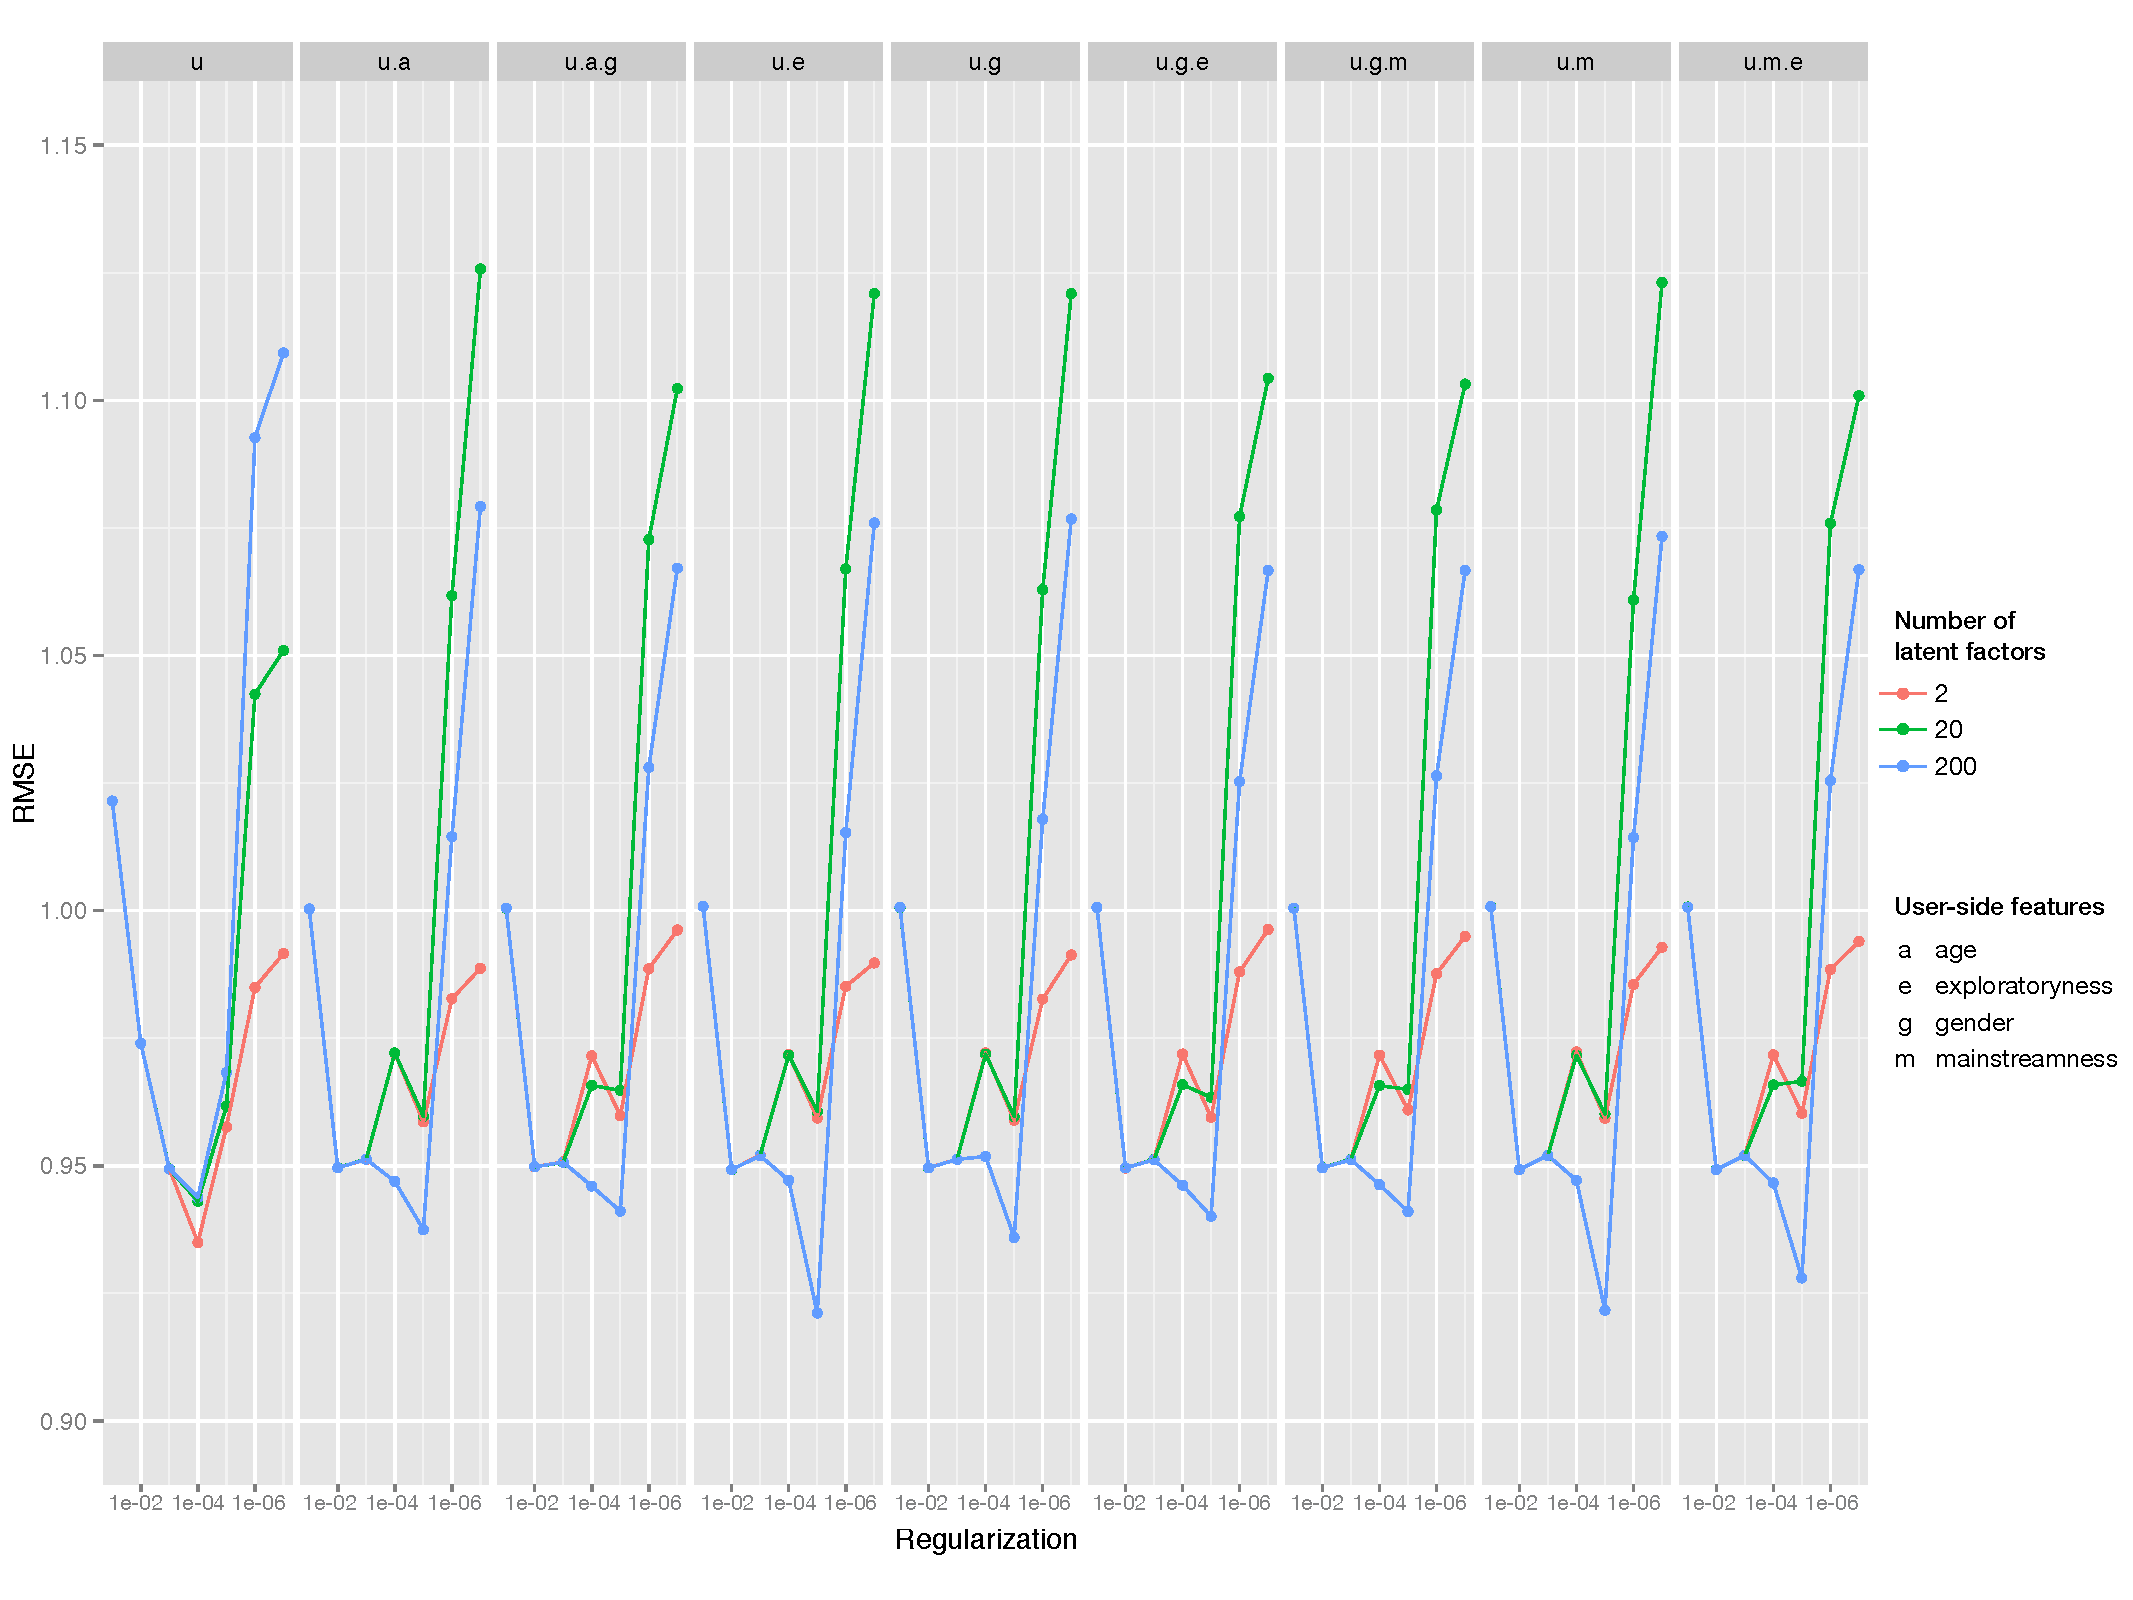
\includegraphics[width = 1.0\textwidth]{Train-test-RMSE-regularization-side-data_200_factors_3_K.pdf}
% \caption{Accuracy of the matrix factorization model. The plot shows root-mean-square error (lower is better) of each of selected nine different user-side features, evaluated with seven different regularization values, and three different number of latent factors. 
% Better accuracy was obtained by using increasing the dimensionality of the model to 200 latent factors, a regularization value of \num{1e05}, and using user's \emph{profiling} instead of \emph{demographics} features}
% \label{fig:Train-test-RMSE-regularization-side-data_200_factors}
% \end{figure}


% Fig.~\ref{fig:Train-test-RMSE-regularization-side-data_200_factors} shows a subset of nine feature combinations, for different regularization values, evaluated with 2, 20, and 200 latent factors. The first column \emph{u} corresponds to the results obtained with no user-side data for estimating the model, just plain matrix factorization with the known implicit feedback of users on artists. 
% As can be seen in the plot, the best RMSE value for the testing set (lower is better) was achieved in several trials by using the profiling features \emph{artist exploratoryness} and \emph{artist mainstreamness} alone, or in their combination, with no demographic features at all. Both features achieved almost the same error value of $.921$ with 200 latent factors and a $lambda$ regularization value of \num{1e-05}.

% These results show that there is not much relevant information in the demographics features to estimate a better prediction model. 
% This lack of impact of the demographics features is intriguing, since it was expected that age, country, or gender would have an effect in reducing the error of a model or, more clearly, in determining the preference of listeners for certain music items.
% On the contrary, there is some information encoded in the listeners' profiling features that help to estimate a better prediction model. 
% However, instead of thinking that demographics data is not relevant, it might be argued that collaborative filtering already has encoded, or expresses, some of the relations between users and their demographics, and so these features do not have a great impact in reducing the error. In other words, latent factors among users may have already some demographics data incorporated in it.

% % Some questions:
% % \begin{itemize}
% % \item The same results will be achieved if I run the test again?
% % \item In a bigger set?
% % \item How factorization machines predict ratings in a toy example? For example, by having people from the same, and different countries
% % \item What features from the item side could be used to improve recommendation? Artists' genre tags? Track' AB data?
% % \end{itemize}



% \subsubsection{Estimating preference model with weekly-aggregated listening data}


% Hypothesizing that people may have different listening preference patterns per music items on weekdays and weekends, we designed an experiment to determine if estimating a model using listening data from weekdays or weekends only, instead of full-week aggregated data, would return lower root-mean-square error values. 
% Hence, when computing RMSE of the estimated model with the testing dataset generated lower values with splits of the weekly listening data, instead of using the full week, that would imply that listeners have different listening preferences between weekdays and weekends because there would be less variance in their listening preferences in the two conditions.

% To test the hypothesis, we took a randomly sample 10 percent of listening histories from our full dataset, considering the artists they listened to. Three sub-datasets of listening histories were generated from this sample.
% The first dataset considered all listening data for all listeners, the second dataset only considered data from weekdays. Finally, the third dataset only considered weekend data. For the three datasets, and for each listener, a ranking of listening preference was generated, and a 5-level likert scale rating value was estimated from the frequency of listening per artist. Table~\ref{table:weekly_aggregated_listening_data} shows the total number of listeners and artists, and the total number of observations, i.e., the total number of implicit feedback-generated ratings.

% \begin{table}[ht]
% \vspace{1em}
% \centering
% 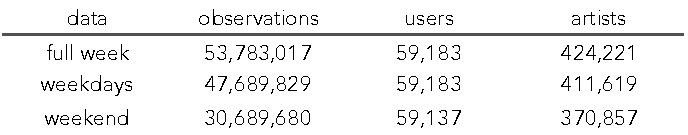
\includegraphics[width = 0.75\textwidth]{experiment_table.pdf}
% \caption{Number of total observations, users, and artists for the different splits of weekly aggregated listening data}
% \label{table:weekly_aggregated_listening_data}
% \end{table}

% From the table, it is possible to see that although the number of listeners is 10 percent of the total number of listeners in the original dataset, the coverage of artists is much larger---being close to 76 percent in the full week and 67 percent on the weekends---since the total number of artists in the dataset is 555K, as was shown in Table~\ref{table:dataset_summary}. This coverage implied that many artists were covered in the sub-datasets notwithstanding the small sample of listeners.


% Again, our procedure followed the approach by \textcite{hu08collaborative}, by factorizing the matrix of observations by two lower-dimensional matrices with a small number of latent factors, with the idea of minimizing the RMSE between the original preference matrix and the product of the two lower dimensional matrices. This procedure was repeated for the three datasets of the experiment. Several different $lambda$ regularization values as well as number of factors were tested in the model estimation in order to obtain the best set of variables for these datasets. 

% Fig.~\ref{fig:weekly_listening_experiment} shows the RMSE values for the training and testing datasets. 

% The chosen method for estimating the models was matrix factorization was Adagrad (Adaptive Stochastic Gradient Descent). The best RMSE values, overall, were found with a $lambda$ of \num{1e-6}.

% % \begin{figure}[h]
% % \centering
% % \includegraphics[width = 1.0\textwidth]{week_weekly_results.pdf}
% % \caption{Number of total observations, users, and items for the different splits of weekly aggregated listening data}
% % \label{fig:week_weekly_results}
% % \end{figure}




% \begin{figure}[ht]
% \vspace{1em}
% \centering
% 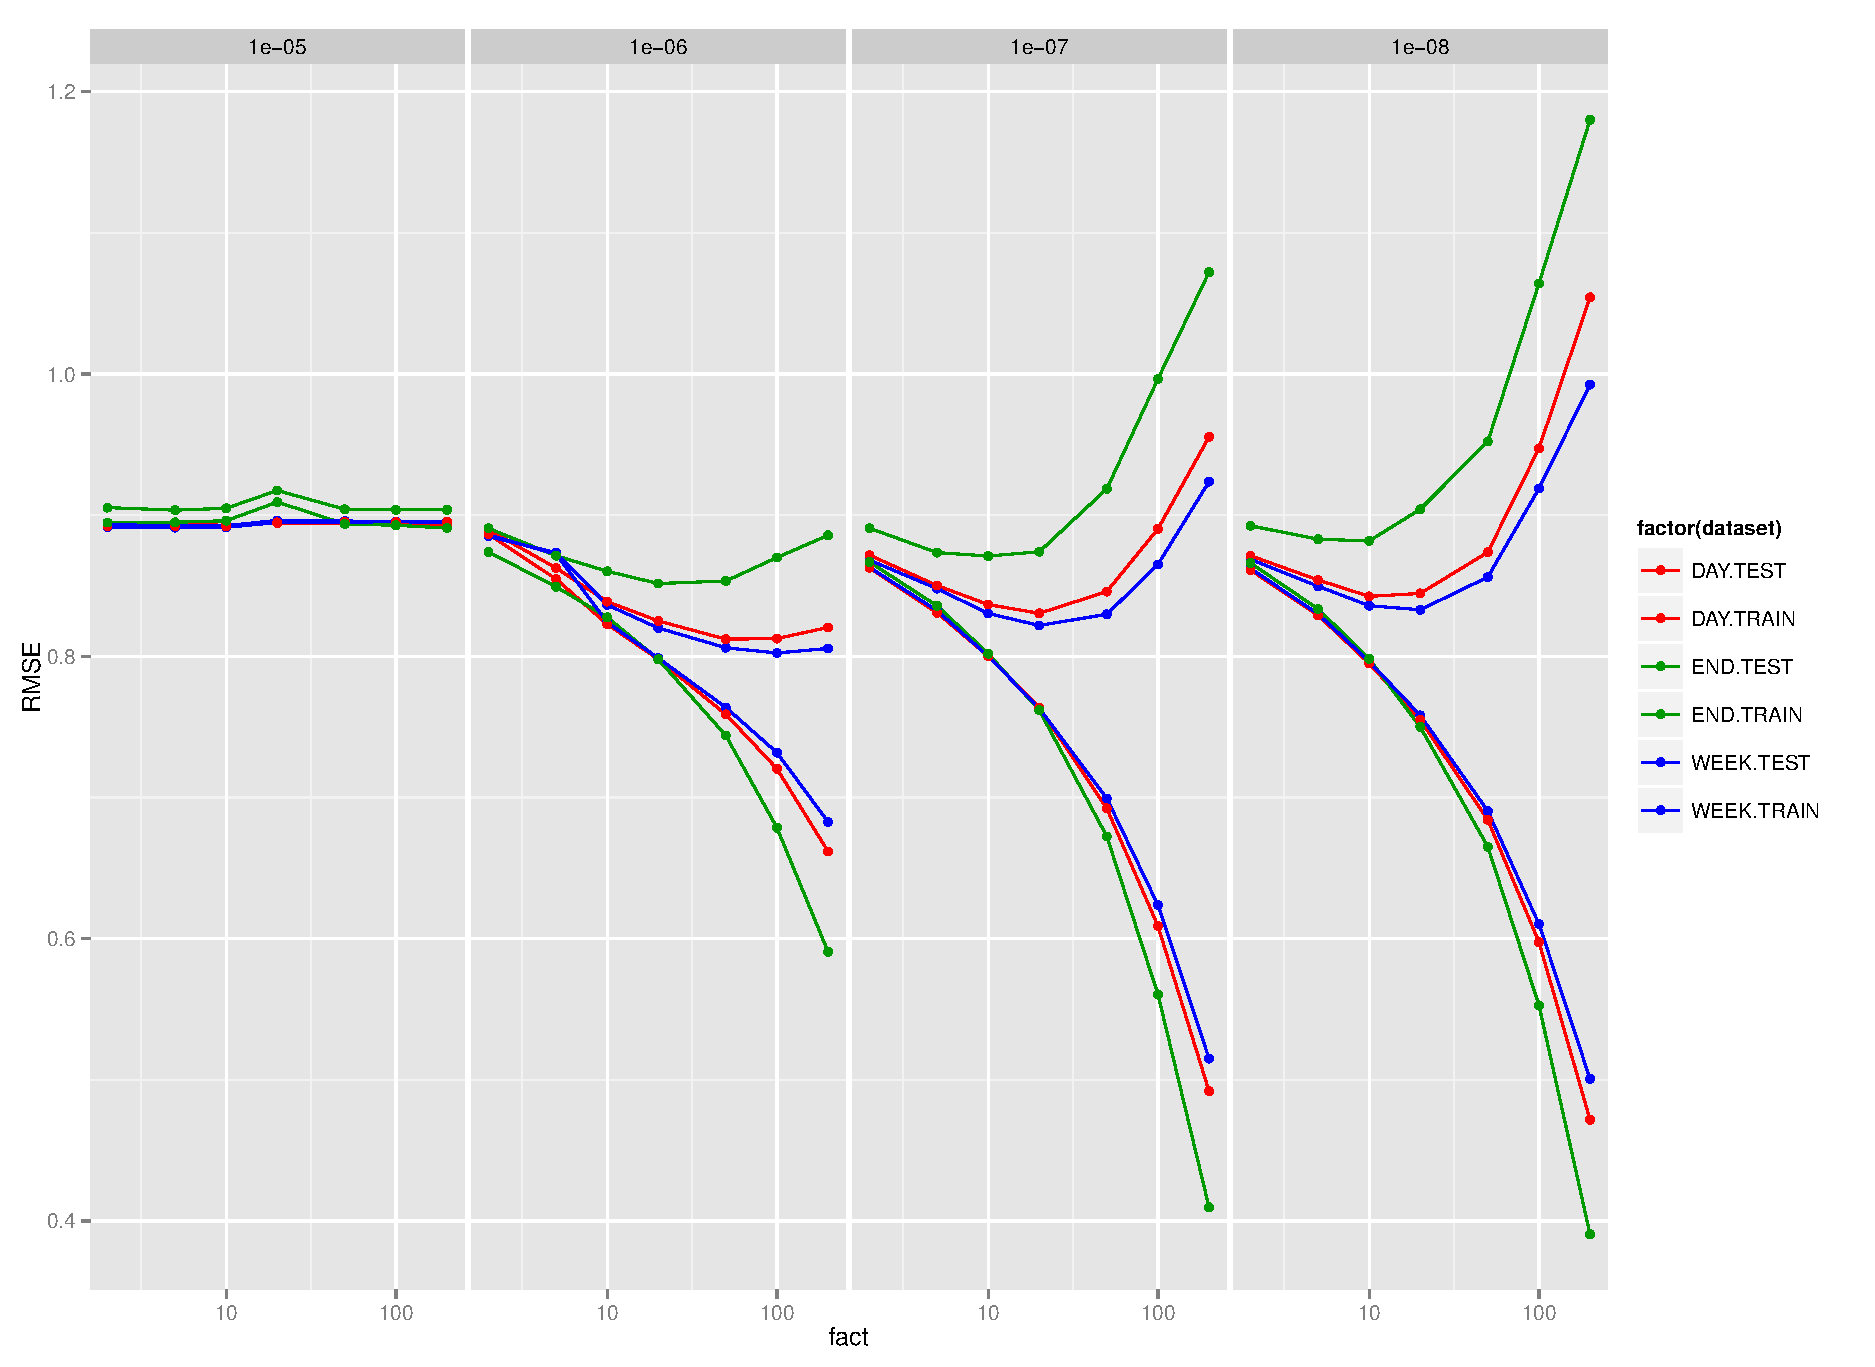
\includegraphics[width = 1.0\textwidth]{weekly_listening_experiment.pdf}
% \caption{Accuracy of the matrix factorization model. The plot shows root-mean-square error of training and testing datasets, for full week, weekdays, and weekend data, evaluated with seven different regularization values, and three different number of latent factors. 
% Better accuracy in the testing dataset was achieved by using the full week data, for all regularization values and number of factors.}
% \label{fig:weekly_listening_experiment}
% \end{figure}


